% !Mode:: "TeX:UTF-8"
\documentclass[linespread=1.5,openany]{book}%任意页开启
\usepackage{xeCJK}
% ========== 超链接 & PDF 书签处理 ==========
\usepackage[colorlinks, linkcolor=black, unicode]{hyperref} % 修改 linkcolor 为 black
\pdfstringdefDisableCommands{%
	\def\R{R}%
	\def\C{C}%
	\def\Z{Z}%
	\def\N{N}%
	\def\diff{d}%
}
\usepackage{tikz}%画图测试
\usepackage{graphicx}%插入图片
\usepackage{enumitem}%用于介绍lecture3
\usepackage{fixltx2e} % 用于文本模式下的下标
\usepackage{amsmath} % 提供数学公式支持,用于标签
\usepackage{amssymb}%用于整数等符号
%引理,定理
\usepackage{amsthm}
\usepackage{booktabs}%\midrule;\bottomrule\toprule
% ========== 定理环境 ==========
\theoremstyle{plain}
% 定义 Theorem 环境
\newtheorem{theorem}{Theorem}
% 定义 Lemma 环境,并与 Theorem 共享编号
\newtheorem{lemma}[theorem]{Lemma}
% 定义 Proof 环境
\newtheorem{corollary}{corollary}
\newtheorem{definition}{Definition}
\newtheorem{proposition}[theorem]{命题}
\newtheorem{example}[theorem]{示例}
%book要改这段代码:(已插入)\renewcommand{\refname}{参考文献}
\renewcommand{\bibname}{参考文献}
%数字编号、排序且压缩、上标、外侧方括号
\usepackage[numbers,sort&compress,super,square]{natbib}
\title{积分变换}
\author{Qiuhui Chen}
\date{}
%用于改变目录深度显示
\setcounter{tocdepth}{4}
% ========== 数学命令 ==========
\newcommand{\diff}{\mathop{}\!\mathrm{d}}  % 微分符号
\newcommand{\R}{\mathbb{R}}                % 实数集
\newcommand{\C}{\mathbb{C}}                % 复数集
\newcommand{\Z}{\mathbb{Z}}                % 整数集
\newcommand{\N}{\mathbb{N}}                % 自然数集
\DeclareMathOperator{\supp}{supp}           % 支持集符号
\renewcommand{\contentsname}{目录}%begin之前使用
\renewcommand{\listfigurename}{插图目录}
\renewcommand{\listtablename}{表格目录}
\renewcommand{\refname}{参考文献}
\renewcommand{\indexname}{索引}
\renewcommand{\tablename}{表}
\renewcommand{\figurename}{图}
%一系列的处理代码
\begin{document}%看起来就是需要maketitle才能正常运行上面的title
	{\maketitle{}
		%这样的命令并不是环境,导入\usepackage{bookmark}即可
		\addcontentsline{toc}{part}{序}%将带星号的部分等插入目录
		%自动生成目录
		\tableofcontents
		\frontmatter{本文旨在将纸质笔记Latex化,方便复习
			\\
			\begin{center}
				\textbf{未经作者允许禁止用于商业活动}\end{center}
			
			
		}
		%\part*{序}%特殊技巧不会显示在目录内
		%本文旨在将纸质笔记Latex化,方便复习
		%正文的输出,页码会是阿拉伯数字
		\mainmatter
	
			
		}
		\part{Lecture 3 Fouier级数敛散性}{
			
			\chapter{敛散性历史}
			{
				(I)\textbf{Fourier 的发现(1807年)}:首次提出 Fourier 级数理论,并认为其收敛性在物理问题中是自然成立的。\\
				(II) \textbf{Dirichlet 的贡献(1829年)}:提出 Dirichlet 条件,证明了满足该条件的周期函数其 Fourier 级数逐点收敛。但当时普遍误认为所有连续函数的 Fourier 级数均收敛。\\
				(III) \textbf{Du Bois-Reymond 的反例(1873年)}:构造了一个连续周期函数,其 Fourier 级数在某一点发散,这一结果颠覆了当时的认知。\\
				(IV) \textbf{Kolmogorov 的工作(1926年)}:证明存在 $L^1\mathbb{[-\pi,\pi)}$ 函数,其 Fourier 级数在每一点都发散。\\
				(V) \textbf{Carleson 的突破(1966年)}:证明了 $L^2\mathbb{[-\pi,\pi)}$ 函数的 Fourier 级数几乎处处收敛:
				\[	S_n(f,x) \rightarrow f(x), \quad \text{a.e.} \ x \in \mathbb{[-\pi,\pi)}.\]
				(VI) \textbf{Hunt 的推广(1967年)}:将结果扩展至 $L^p(\mathbb{[-\pi,\pi)})$ 空间($p>1$),证明对任意 $f \in L^p\mathbb{[-\pi,\pi)}$,有:
				\[
				S_n(f,x) \rightarrow f(x), \quad \text{a.e.} \ x \in \mathbb{[-\pi,\pi)}.
				\]
				世界性难题解决!\\
				注:(i)Carleson 的证明极其复杂,但其结论(Carleson-Hunt 定理)奠定了现代 Fourier 分析的基石。\\
				(ii)连续函数的 Fourier 级数收敛性问题并非完全解决,例如是否存在连续函数其 Fourier 级数在某个正测集上发散,仍是未解之谜。\\
				(iii)这些成果深刻影响了调和分析、偏微分方程及信号处理等领域。
			}
			\chapter{求和理论初步}
			{
				\section{一些和}{
					\subsection{Fejér 求和法(算术平均求和法)}
					{定义 Fejér 和为:\[
						\sigma_n(x) = \frac{1}{n+1} \sum_{k=0}^n S_k(f,x) = \frac{1}{n+1} \sum_{k=-n}^n \left( 1 - \frac{|k|}{n+1} \right) C_k e^{ikx}
						=\frac{1}{n+1}\sum_{k=0}^nf*\varrho_k\]
						则其积分形式可表示为:
						\[
						\sigma_n(x) = \frac{1}{2\pi(n+1)} \int_{-\pi}^{\pi} f(x-t) \left( \frac{\sin\left( \frac{(n+1)t}{2} \right)}{\sin\left( \frac{t}{2} \right)} \right)^2 dt
						\]\[ \int_{-\pi}^{\pi} f(x-t)K_n(t) dt\]
						\[\textbf{Fej\'{e}r核:}K{(t)}= \frac{1}{2\pi(n+1)}(\frac{\sin \frac{(n+1)t}{2} }{\sin  \frac{t}{2}  }  )^2\]
					}
					\subsection{Abel 求和与 Poisson 核}
					{定义 Abel-Poisson 和为:
						\[
						F(r,x) = \sum_{k=-\infty}^{\infty} C_k r^{|k|} e^{ikx} = \frac{1}{2\pi} \int_{-\pi}^{\pi} f(t) P(r, x-t) dt,
						\]
						其中 Poisson 核为:
						\[
						P(r, t) \stackrel{\textbf{负号变正,通分}}{=}\frac{1}{2} \frac{1 - r^2}{1 - 2r\cos t + r^2} =\frac{1}{2}+ \sum_{n=1}^\infty r^{n} e^{int}.
						\]
						注:(i) \textbf{解析性}:当 $r \to 1^-$ 时,$F(r,x)$ 在单位圆内解析,边界值与原函数相关。\\
						(ii) \textbf{收敛性}:若 $f \in L^p(\mathbb{E}) \ (p \geq 1)$,则 $F(r,x) \to f(x) \ \text{a.e.}$ 当 $r \to 1^-$。\\
					}
				}
				{
					\section{Lebesgue定理}
					\begin{theorem}[Lebesgue]
						若 $f \in L^1\mathbb{[-\pi,\pi)}$且$f$ 在 $x_0$ 处满足 Lebesgue 条件:
						\[\lim_{h \to 0} \frac{1}{h} \int_0^h |f(x_0 + t) - f(x_0)| dt = 0,\]
						\item[(i)]
						$\sigma_n(x_0) \to f(x_0) \ (n \to \infty)$
						\item[(ii)]在几乎处处意义下,$\sigma_n(x) \to f(x) \ \text{a.e.} \ x \in \mathbb{[-\pi,\pi)}$.
					\end{theorem}
					\begin{theorem}[$L^p$ 收敛性]
						若 $f \in L^p\mathbb{[-\pi,\pi)}$ 且 $1 \leq p < \infty$,则:
						\[
						\lim_{n \to \infty} \| f - \sigma_n(f) \|_p = 0.
						\]
					\end{theorem}
			}}
			\chapter{Fourier级数的收敛性}{
				\section{基本定义与部分和}
				{设 \( f \in L^1[-\pi, \pi] \) 为广义周期函数,其 Fourier 部分和为:
					\[
					S_n(f, x) = \frac{a_0}{2} + \sum_{k=1}^n \left( a_k \cos kx + b_k \sin kx \right),
					\]
					其中系数由积分表达式给出:
					\[
					a_k = \frac{1}{\pi} \int_{-\pi}^{\pi} f(u) \cos(ku) \, du, \quad 
					b_k = \frac{1}{\pi} \int_{-\pi}^{\pi} f(u) \sin(ku) \, du.
					\]于是:
					\[S_n(f, x) = \frac{1}{2\pi} \int_{-\pi}^{\pi} f(u) \, du + \frac{1}{\pi} \sum_{k=1}^n \int_{-\pi}^{\pi} f(u) \cos k(u-x) \, du.
					\]进一步化简为:\[
					S_n(f, x) = \frac{1}{\pi} \int_{-\pi}^{\pi} f(u) \left( \frac{1}{2} + \sum_{k=1}^n \cos k(u-x) \right) du.
					\]
					利用三角恒等式:
					\[
					\frac{1}{2} + \sum_{k=1}^n \cos k\theta = \frac{\sin\left( (n+\frac{1}{2})\theta \right)}{2 \sin \frac{\theta}{2}},
					\]
					可得 Dirichlet 核表示:
					\[S_n(f, x) = \frac{1}{\pi} \int_{-\pi}^{\pi} f(u) \cdot \frac{\sin\left( (n+\frac{1}{2})(u-x) \right)}{2 \sin \frac{u-x}{2}} \, du.
					\]
					令$u=x+t$,则:
					\[S_n(f, x) = \frac{1}{\pi} \int_{-\pi-x}^{\pi-x} f(x+t) \frac{\sin\left( (n+\frac{1}{2})t \right)}{2 \sin \frac{t}{2}} \, dt.\]\\
					\begin{align}{
							&= \frac{1}{\pi} \int_{-\pi}^{\pi} f(x-t) \frac{\sin\left( (n+\frac{1}{2})t \right)}{2 \sin \frac{t}{2}} \, dt.\label{3.1.1}
					}\end{align}
					定义Dirichlet核:
					\begin{align}{
							D_n(t) &= \frac{1}{2\pi}\frac{\sin\left( (n+\frac{1}{2})t \right)}{\sin \frac{t}{2}} \label{3.1.2}	
					}\end{align}
					\subsection{dirichlet核性质}
					{ \textbf{归一性}:
						\[\int_{-\pi}^{\pi} D_n(t) dt = 1.\]
						\textbf{偶性}:
						\[	D_n(-t) = D_n(t).\]
						\textbf{正交投影}:$S_n$是从$L^2(\mathbb{E})$到$2n+1$维三角多项式空间的投影算子,即
						\[S_n: L^2(\mathbb{E}) \to \mathcal{T}_n, \quad \mathcal{T}_n = \mathrm{span}\{ e^{ikx} \}_{k=-n}^n.\]}
					\subsection{复指数的化简}{$f \in L^1(\mathbb{E})$的Fourier部分和可表示为:
						\[S_n(f, x) = \sum_{k=-n}^n C_k e^{ikx} = \frac{1}{2\pi} \int_{-\pi}^{\pi} f(u) \sum_{k=-n}^n e^{ik(x-u)} du\]
						其中复数系数为:
						\[C_k = \frac{1}{2\pi} \int_{-\pi}^{\pi} f(u) e^{-iku} du.\]
						\[S_n(f, x) = \frac{1}{2\pi} \int_{-\pi}^{\pi} f(u) \frac{e^{-in(x-u)}-e^{in(x-u)}e^{i(x-u)}}{1-e^{-i(x-u)}}du\]
						\[= \frac{1}{2\pi} \int_{-\pi}^{\pi} f(u)e^{\frac{i(x-u)}{2}} \frac{e^{-i(n+\frac{1}{2})(x-u)}-e^{i(n+\frac{1}{2})(x-u)}e^{i(x-u)}}{(e^{\frac{i(x-u)}{2}})(e^{-\frac{i(x-u)}{2}}-e^{\frac{i(x-u)}{2}})}du\]
						\[= \frac{1}{2\pi} \int_{-\pi}^{\pi} f(u) \frac{\sin(n+\frac{1}{2})(x-u)}{\sin (x-u)}du \]
						$$=f*D_n(u)$$
					}
				}
				\section{收敛性}{
					\subsection{技术性处理}{
						问题直接归结于$\{S_n\}$的敛散性,如果存在极限,那么假设偏差量:
						\[S_n(f, x) - c = \int_{-\pi}^{\pi} \left( f(x-t) - c \right) D_n(t) \, dt,\]
						将正负分开换元得到:
						\begin{align}{S_n(f, x) - c = \int_{0}^{\pi} \left[ f(x-t) + f(x+t) - 2c \right] D_n(t) \, dt. \label{3.1.3}}
						\end{align}
						记 \(\psi_x(t) = f(x+t) + f(x-t) - 2c\),且 \(\psi_x(-t) = \psi_x(t)\)。 \(\psi_x(t) \in L^1(0, \pi)\)由$f$控制,则有:
						\[
						\int_0^\pi \psi_x(t) \, dt = \int_0^\pi f(x+t) \, dt + \int_0^\pi f(x-t) \, dt - 2c\pi.\]
						\[S_n(f, x) - c = \int_{0}^{\pi}  \psi_x(t) D_n(t) \, dt.\]	
						\[= \int_0^\pi \psi_x(t) \cdot \frac{\sin(nt) \cos \frac{t}{2} + \cos(nt) \sin \frac{t}{2}}{2\pi \sin \frac{t}{2}} \, dt.\]
						\[
						= \int_0^\pi \psi_x(t) \cdot \frac{\cos \frac{t}{2} \sin nt}{2\pi \sin \frac{t}{2}} \, dt + \frac{1}{2\pi} \int_0^\pi \psi_x(t) \cos(nt) \, dt.
						\]
						Riemann-Lebesgue引理告诉我们第二项在\(n \to \infty\) 时为o(1)故只需关注:
						\begin{align}{
								&= \frac{1}{2\pi} \int_0^\pi \psi_x(t) \cos \frac{t}{2} \cdot \frac{\sin nt}{\sin \frac{t}{2}} \, dt\label{3.1.4}}\end{align}}
					\subsection{奇点的处理}{问什么情况下\ref*{3.1.4}趋于0?一个自然的想法是尽可能的运用Riemann-Lebesgue引理:我们设$\forall \delta \in(0,\frac{\pi}{2})$
						\[\frac{1}{2\pi} \int_0^\pi \psi_x(t) \cdot \frac{\cos \frac{t}{2} \sin nt}{\sin \frac{t}{2}} \, dt\]
						\[=\frac{1}{2\pi} \int_0^\delta \psi_x(t) \cdot \frac{\cos \frac{t}{2} \sin nt}{\sin \frac{t}{2}} \, dt+\frac{1}{2\pi} \int_\delta^\pi \psi_x(t) \cdot \frac{\cos \frac{t}{2} \sin nt}{\sin \frac{t}{2}} \, dt\]
						因此第二项使用Riemann-Lebesgue引理后,充分条件即为:
						\[S_n(f, x) \to c \quad (n \to \infty) \quad \Leftrightarrow \quad \int_0^\delta \psi_x(t)  \frac{\cos \frac{t}{2}}{\sin \frac{t}{2}} \sin nt \, dt \to 0 \quad (n \to \infty).
						\]
						下面的Dini条件告诉我们$\delta \in(0,\pi)$满足一定条件下只需要一个即可
					}
					\subsection{Fouier级数收敛第一充分条件(Dini)}{
						\begin{theorem}\label{3.2.theorem.DINI}
							{$f \in L^1(\mathbb{E})$,$C \in \mathbb{C}$ 为常数。偏差函数:
								\[
								\psi_x(t) = f(x+t) + f(x-t) - 2c,
								\]
								若存在 $\delta > 0$ 使得:
								\[
								\int_0^\delta \frac{|\psi_x(t)|}{t} \, dt < \infty.
								\]
								则\[
								\lim_{n \to \infty} S_n(f, x) = C.
								\]}
						\end{theorem}
						\begin{proof}
							{考虑$$\int_0^\delta \psi_x(t)  \frac{\cos \frac{t}{2}}{\sin \frac{t}{2}} \sin nt \, dt$$
								显然$$\frac{\psi_x(t)}{t} \subset {L^1(0,\delta)}$$
								\[ \text{利用}\frac{t\cos \frac{t}{2}}{\sin \frac{t}{2}}\text{在} (-\infty,\infty)\text{的连续性}\]
								使用Riemann-Lebesgue引理得证}
						\end{proof}
						\begin{theorem}[推论1]{设 \( f \in L(-\pi, \pi) \),若 \( f \) 在 \( x \) 处可微,则 \( S_n(f, x) \to f(x) \) (\( n \to \infty \))}
						\end{theorem}
						\begin{proof}{
								在定理10中,令 \( c = f(x) \)。
								定义:\[\psi_x(t) = f(x+t) + f(x-t) - 2f(x).\] 
								\[\Rightarrow\frac{\psi_x(t)}{t} = \frac{f(x+t) - f(x)}{t} + \frac{f(x-t) - f(x)}{ t}.\]
								
								\[= \frac{f(x+t) - f(x)}{t} - \frac{f(x-t) - f(x)}{-t}.\]
								当 \( t \to 0 \) 时:
								\[\lim_{t \to 0} \frac{\psi_x(t)}{t} = f'(x) - f'(x) = 0.\]
								因此,若:\[
								\int_0^\delta \frac{|\psi_x(t)|}{t} \, dt < \infty,\]
								\textbf{note:} \(\forall \varepsilon > 0\),存在 \(\delta_1 > 0\),当 \( t \in (0, \delta_1) \) 时:
								\[
								\left| \frac{\psi_x(t)}{t} \right| < \varepsilon.
								\]
								同样的思想,第二项由Riemann-Lebesgue引理控制,第一项是经典分析学的内容:
								\[\int_0^\delta \frac{|\psi_x(t)|}{t} \, dt\]
								\[=\int_0^{\delta_{1}} \frac{|\psi_x(t)|}{t} \, dt+\int_{\delta_{1}}^\delta \frac{|\psi_x(t)|}{t} \, dt\ \]
								\[ \le \varepsilon\delta_{1}+\int_{\delta_{1}}^\delta \frac{|\psi_x(t)|}{t} \, dt \to o(1)\]
						}\end{proof}
						
						\begin{theorem}[推论2]{设 \( f \in L(-\pi, \pi) \),若 \( f \) 在 \( x \) 处满足Lipschitz条件,即存在常数 \( M > 0 \) 和 \( \alpha \in (0, 1] \),使得:
								\[
								|f(x+t) - f(x)| \leq M |t|^\alpha \quad  \alpha \in (0, 1].
								\]
								
								则 \( S_n(f, x) \to f(x) \) (\( n \to \infty \))}
						\end{theorem}
						\begin{proof}
							{这是显然的:使用(\textbf{Theorem}\ref{3.2.theorem.DINI}):\[	\psi_x(t) = f(x+t) + f(x-t) - 2f(x).	\]
								则:\[\left| \frac{\psi_x(t)}{t} \right| \leq \left| \frac{f(x+t) - f(x)}{t} \right| + \left| \frac{f(x-t) - f(x)}{t} \right| \leq 2M |t|^{\alpha - 1}.\]
								因此,积分:\[\int_0^\delta \frac{|\psi_x(t)|}{t} \, dt \leq 2M \int_0^\delta |t|^{\alpha - 1} \, dt < \infty.\]}
						\end{proof}
						注:这种推论可以构造很多条件,只需要保证存在 $\delta > 0$ 使得\[\int_{0}^{\delta} \frac{\psi_x(t)}{t} \, dt < \infty \quad \]
						再举一个例子: \( f \in C^2[-\pi, \pi] \) 且满足 Hölder 条件:\[
						|f(x+\epsilon) - f(x)| \leq M \cdot \frac{1}{\left|\ln|x|\right|^{\epsilon+1}} \quad (\epsilon > 0)\]则 
						\[S_n(f, x) \to f(x) \quad (n \to \infty).\]即 Fourier 级数在点 $x$ 处收敛于 $f(x)$
					}
					
					\subsection{Fouier级数收敛第二充分条件(Jordan)}{}
					
					先证明一个引理以便行文流畅:
					\begin{lemma}\label{3.2.lemma14}
						{对任意 $a,b \in \mathbb{R}$,有\[\left| \int_a^b \frac{\sin x}{x} dx \right| \leq 6.\]}\end{lemma}
					\begin{proof}
						{当 $1 \leq |a| \leq b$ 时,由第二积分中值定理,存在 $\xi \in [a,b]$ 使得:
							\[	\left| \int_a^b \frac{\sin t}{t} dt \right| = \frac{1}{|a|} \left| \int_a^\xi \sin t dt \right| \leq \frac{2}{|a|} \leq 2.
							\] 当 $0 \leq a \leq b \leq 1$ 时:
							\[
							\left| \int_a^b \frac{\sin t}{t} dt \right| \leq \int_a^b 1 dt = b - a \leq 1.
							\] 综合两种情况可得:
							\[\left| \int_a^b \frac{\sin x}{x} dx \right| \leq 3 \quad \text{(同号积分)}.\] 对于一般情况($a<0<b$):
							\[\left| \int_a^b \frac{\sin x}{x} dx \right| \leq \int_0^{|a|} + \int_0^{|b|} \leq 6.\]
							\textbf{note:}定理并非是必要的甚至可以直接令  $I\leq\frac{\pi}{2}$}
					\end{proof}
					现在来证明Jordan条件:
					\begin{theorem}{设 $f \in L^1[-\pi, \pi]$,且 $f$ 在点 $x$ 的某邻域 $U(x,r)$ 上有界变差,则其Fourier级数部分和满足:	\[\lim_{n \to \infty} S_n(f, x) = \frac{1}{2} \left[ f(x+0) + f(x-0) \right].\]}
					\end{theorem}
					\begin{proof}
						{设 \( f \in BV(x-r, x+r) \),则 \( f(x+0) \) 和 \( f(x-0) \) 存在(Jordan分解定理:因有界变差函数在每点存在单侧极限)换句话说:
							存在单调递增函数 \( g, h \) 使得:
							\[ \psi_x(t) = g(t) - h(t)\]
							\[ g(x+0) =\textbf{inf}\begin{Bmatrix}
								g
							\end{Bmatrix} \]
							\[ {h}(x+0) =\textbf{sup}\begin{Bmatrix}
								h
							\end{Bmatrix} .\]定义:
							\[
							c = \frac{1}{2} \left( f(x+0) + f(x-0) \right) 
							\] 
							\[\text{则}
							\psi_x(t) = f(x+t) + f(x-t) - f(x+0) - f(x-0)\in B.V(-r,r)
							\]
							\[\Rightarrow\text{存在单调递增函数 \( h_1, h_2 \) 使得:}
							\psi_x(t) \stackrel{\text{Jordan分解}}{=} h_1(t) - h_2(t)\]\[\text{且(极限形式)} \quad h_1(0+0) = h_2(0+0) = 0(\because \psi_x (0+0)=0)
							\] 
							\begin{align}{\text{则}
									S_n(f, x) - c = \frac{1}{2\pi} \int_0^\delta \psi_x(t) \cdot \frac{\sin\left( (n+\frac{1}{2})t \right)}{\sin\left( \frac{t}{2} \right)} dt + o(1) \label{3.1.5} }
							\end{align}\[
							\text{取$n$足够大}\Rightarrow |o(1)|<\varepsilon\]
							$\varepsilon-\delta$语言告诉我们:$\forall \varepsilon>0,\exists \delta<r,$使得$t\in(0,\delta),0\le h_j\le\varepsilon $ \\
							重新考虑(\ref{3.1.5})只需要估计Dirichlet核即可,使用引理(\textbf{Lemma}\ref{3.2.lemma14})和积分第二中值定理:
							\[	\left| S_n(f, x) - C \right| \leq \left| \frac{1}{\pi} \int_0^\delta h_1(t) \frac{\sin(nt)}{t} \, dt \right| + \left| \frac{1}{\pi} \int_0^\delta h_2(t) \frac{\sin(nt)}{t} \, dt \right| + \varepsilon \]
							\[= \left| \frac{1}{\pi} h_1(\delta) \int_{\xi_1 }^{\delta} \frac{\sin(nt)}{t} \, dt \right| + \left| \frac{1}{\pi} h_2(\delta) \int_{\xi_2}^{\delta} \frac{\sin(nt)}{t} \, dt \right| + \varepsilon \\
							\leq \left( \frac{6+6}{\pi} \right) \varepsilon + \varepsilon \]
							\[= \left( 1 + \frac{12}{\pi} \right) \varepsilon\]
						}
					\end{proof}
				}
				\section{补充资料}
				{
					\subsubsection{积分第二中值定理}
					\begin{theorem}
						{设 \( f \) 在 \([a, b]\) 上Riemann可积。若 \( g \) 在 \([a, b]\) 上递减且 \( g(x) \geq 0 \),则存在 \(\xi \in [a, b]\),使得:\[\int_a^b f(x) g(x) \, dx = g(a) \int_a^\xi f(x) \, dx.	\]
							若 \( g \) 在 \([a, b]\) 上递增且 \( g(x) \geq 0 \),则存在 \(\eta \in [a, b]\),使得:\[\int_a^b f(x) g(x) \, dx = g(b) \int_\eta^b f(x) dx\]
						}
					\end{theorem}
					\subsubsection{为什么选择Dirichlet核}
					{\[\int_0^\delta \psi_x(t) \cot \frac{t}{2} \sin nt \, dt\]
						转换为:\[\int_0^\delta \frac{\psi_x(t)}{t} \sin nt \, dt\]
						是基于以下分析,定义函数 \( g(t) \) 如下:
						\[g(t) \stackrel{\Delta}{=} \begin{cases} \cot \frac{t}{2} - \frac{1}{t}, & t \in [-\pi, \pi] \setminus \{0\} \\0, & t = 0
						\end{cases}
						\]在 \([- \pi, \pi]\) 上连续\\
						证明是容易的,注意到分母是1阶的,而分子有2阶以上的余项}
					\subsubsection{数学分析中的经典收敛定理}{
						\begin{theorem}[Dirichlet收敛定理]
							(i)设函数 $f$ 在区间 $[-\pi, \pi]$ 上满足:分段光滑\\
							(ii)在 $[-\pi, \pi]$ 上除有限个第一类间断点外连续
							则对任意 $x \in (-\pi, \pi)$,其Fourier级数部分和满足:
							\[	S_n(x) \to \frac{f(x+0) + f(x-0)}{2} \quad (n \to \infty)	\]
						\end{theorem}
						\begin{proof}{
								定义偏差积分:
								\[
								\int_0^\delta \frac{\psi_x(t)}{t} \sin(nt) \, dt = \int_0^\delta \frac{f(x+t)-f(x+0)}{t} \sin(nt) \, dt + \int_0^\delta \frac{f(x-t)-f(x-0)}{t} \sin(nt) \, dt
								\]
								其中定义辅助函数:
								\[
								\begin{aligned}
									\varphi_1(t) = \frac{f(x+t)-f(x+0)}{t}, \quad t \in (0, \delta] \\
									\varphi_2(t) = \frac{f(x-t)-f(x-0)}{t}, \quad t \in (0, \delta]
								\end{aligned}
								\] 
								关于正则性分析:
								在 $t \to 0^+$ 时(分段光滑保证左右导数存在)
								\[\varphi_1(0^+) = \lim_{t \to 0^+} \frac{f(x+t)-f(x+0)}{t} = f'(x^+)\]
								\[\varphi_2(0^+) = \lim_{t \to 0^+} \frac{f(x-t)-f(x-0)}{t} = -f'(x^-)\]
								$\varphi_1, \varphi_2$ 在 $[0, \delta]$ 上连续(可数个第一类间断点其他都是连续点)
								
								
								应用Riemann-Lebesgue引理
								\[\int_0^\delta \varphi_i(t) \sin(nt) \, dt = o(1) \quad (n \to \infty),\quad i=1,2\]
								因此原积分满足:
								\[\int_0^\delta \frac{\psi_x(t)}{t} \sin(nt) \, dt = o(1) \quad (n \to \infty)\]
						}\end{proof}
						评注:现在回顾来看观点有点低了
					}
				}
			}
		}
		\part{Lecture 4 Fourier 变换}{
			\chapter{级数到变换的形式推演}
			{\section{代数运算}
				若 \(f \in L^{1}(-\ell,\ell)\) ,则 \(f \sim \sum_{k = -\infty}^{\infty} C_{k}e^{i k \frac{\pi}{\ell} x}\) ,其中 \(C_{k} = \frac{1}{2\ell}\int_{-\ell}^{\ell} f(t)e^{-i k \frac{\pi}{\ell} t} dt\) 。
				
				那么 \[\sum_{k \in \mathbb{Z}} c_{k}e^{i k \frac{\pi}{\ell} x}\]
				\[
				= \sum_{k \in \mathbb{Z}} \left(\frac{1}{2\ell}\int_{-\ell}^{\ell} f(y)e^{-i k \frac{\pi}{\ell} y} dy\right) e^{i k \frac{\pi}{\ell} x}
				\]
				\[
				= \sum_{k \in \mathbb{Z}} \frac{1}{2\ell} \int_{-\ell}^{\ell} f(y) e^{i k \frac{\pi}{\ell}(x - y)} dy
				\]
				\[
				= \sum_{k \in \mathbb{Z}} \left(\frac{1}{2\pi}\int_{-\ell}^{\ell} f(y) e^{i (k \frac{\pi}{\ell})(x - y)} dy\right) \frac{\pi}{\ell}
				\]
				令 \(t_{k} = k \frac{\pi}{\ell}\) ,则 \(\Delta t_{k} = t_{k + 1} - t_{k} = (k + 1)\frac{\pi}{\ell} - k\frac{\pi}{\ell} = \frac{\pi}{\ell}\) 。
				
				故上述式子可写为
				\[
				= \sum_{k \in \mathbb{Z}} \left(\frac{1}{2\pi}\int_{-\ell}^{\ell} f(y)e^{i t_{k}(x - y)} dy\right) \Delta t_{k}
				\]
				\[
				= \sum_{k \in \mathbb{Z}} g_{\ell}(t_{k})\Delta t_{k} \text{;其中 } g_{\ell} = \frac{1}{2\pi}\int_{-\ell}^{\ell} f(y)e^{i t(x - y)} dy
				\]
				\[
				\approx \int_{-\infty}^{\infty} \left(\frac{1}{2\pi}\int_{-\ell}^{\ell} f(y)e^{i t(x - y)} dy\right) dt
				\]
				\[
				\to \int_{-\infty}^{\infty} \frac{1}{2\pi}\int_{-\infty}^{\infty} f(y)e^{i t(x - y)} dy dt
				\]
				\[
				= \frac{1}{\sqrt{2\pi}}\int_{-\infty}^{\infty} \left(\frac{1}{\sqrt{2\pi}}\int_{-\infty}^{\infty} f(y)e^{-i t y} dy\right) e^{i t x} dt
				\]
				
				令 \[\hat{f}(t) = \frac{1}{\sqrt{2\pi}}\int_{-\infty}^{\infty} f(y)e^{-i t y} dy\] 
				则 \[f(x) \sim \frac{1}{\sqrt{2\pi}}\int_{-\infty}^{\infty} \hat{f}(t) e^{i t x} dt \] 。
				以上是从傅里叶级数到非周期函数的傅里叶变换的形式推导,严格的证明将在不同空间展开。 
				\section{Riemann-Lebesgue引理}
				\begin{theorem}[Riemann-Lebesgue]\label{4.2.riemann-lebesgue}
					\[	\text{若}f \in L^1(\mathbb{R})\text{则}\lim_{|w| \to \infty} \hat{f}(w) = 0\]
					\begin{center} \[ 
						\text{即}\hat{f}(w)=o(1) 	\text{当}|w| \to \infty \](这暗示我们高频幅度可忽略不计)\end{center}
				\end{theorem}
				\begin{proof}
					\begin{itemize}
						\item[(i)] 考虑特征函数:当 \( f = \chi_{[a, b]} \) 时,直接计算其\emph{Fourier变换},这个积分是简单的:
						\[
						\hat{f}(w) = \frac{1}{\sqrt{2\pi}} \int_{a}^{b} e^{-i w t} dt
						\]
						\[= \frac{1}{\sqrt{2\pi}} \cdot \frac{e^{-i w b} - e^{-i w a}}{-i w}
						\]
						\[= \frac{1}{\sqrt{2\pi}} \cdot \frac{e^{-i w b} - e^{-i w a}}{-i w}
						\]
						取绝对值:
						\[
						|\hat{f}(w)| \leq \frac{1}{\sqrt{2\pi}} \cdot \frac{2}{|w|} \to 0 \quad (|w| \to \infty)
						\]
						因此,\( \hat{f}(w) \to 0 \) 当 \( |w| \to \infty \)。
						
						\item [(ii)] 当 \( f \) 是有限个特征函数 \( \chi_{[a_i, b_i]} \) 的线性组合时,利用积分线性性和极限线性性,可知:
						\[
						\hat{f}(w) \to 0 \quad (|w| \to \infty)
						\]
						即紧支撑的分片(或紧支集)常数函数的Fourier变换趋于0( \( |w| \to \infty \) )
						
						\item [(iii)]  \(\forall f \in L^1(\mathbb{R}) \), \(\forall \varepsilon > 0 \),存在一个紧支撑的分片常函数 \( g \),使得:
						\[
						\|f - g\|_1 = \int_{\mathbb{R}} |f(x) - g(x)| dx < \varepsilon
						\]
						
						\item [(iv)]对于 \( f \in L^1(\mathbb{R}) \),分解其\emph{Fourier变换}:
						\[
						\hat{f}(w) = \hat{f}(w) - \hat{g}(w) + \hat{g}(w)
						\]
						\[
						\hat{f}(w) = \frac{1}{\sqrt{2\pi}} \int_{\mathbb{R}} (f(x) - g(x)) e^{-i w x} dx + \frac{1}{\sqrt{2\pi}} \int_{\mathbb{R}} g(x) e^{-i w x} dx
						\]
						记为:
						\[
						\hat{f}(w) = J_1(w) + J_2(w)
						\]
						第一项:	
						\[
						|J_1(w)| \leq \frac{1}{\sqrt{2\pi}} \int_{\mathbb{R}} |f(x) - g(x)| dx \leq \frac{1}{\sqrt{2\pi}} \varepsilon
						\]
						第二项:
						由于 \( g \) 是紧支撑的分片常函数,根据(ii):
						\[|J_2(w)| = o(1) \quad (|w| \to \infty)\]
						所以:\[
						|\hat{f}(w)| \leq |J_1(w)| + |J_2(w)| \leq \frac{1}{\sqrt{2\pi}} \varepsilon + o(1)
						\]	
						令 \( \varepsilon \to 0 \  |w| \to \infty  \) 得
						\[
						\hat{f}(w) \to 0 \quad (|w| \to \infty)
						\]	\end{itemize}
				\end{proof}
				\section{Fourier变换的性质}
				\subsection{线性变换,且可逆}
				略
				\subsection{有界}
				\begin{theorem}
					\[\mathcal{F}\text{是:}L^1(\mathbb{R})\rightarrow L^{\infty}(\mathbb{R})\text{有界线性算子}\]
					\[\forall f \in L^1(\mathbb{R})\Rightarrow|\mathcal{F}[f](\lambda)| \leq \frac{1}{\sqrt{2\pi}} \|f\|_1
					\]
				\end{theorem}
				\begin{proof}
					\[
					\left| \frac{1}{\sqrt{2\pi}} \int_{-\infty}^{+\infty} f(t) e^{-i\lambda t} dt \right|\leq \frac{1}{\sqrt{2\pi}} \int_{-\infty}^{+\infty} |f(t)|\cdot|e^{-i\lambda t}| dt = \frac{1}{\sqrt{2\pi}} \int_{-\infty}^{+\infty} |f(t)| dt = \frac{1}{\sqrt{2\pi}} \|f\|_1
					\]
					因此,若 $f \in L^1(\mathbb{R})$,则 $\mathcal{F}[f] \in L^\infty(\mathbb{R})$,且:
					\[
					\|\mathcal{F}[f]\|_{L^\infty} = \operatorname{ess\,sup} |\mathcal{F}[f](\lambda)| \leq \frac{1}{\sqrt{2\pi}} \|f\|_1 < +\infty
					\]
				\end{proof}
				傅里叶变换将 $L^1$ 空间中的函数映射到 $L^\infty$ 空间中的函数,且变换后的函数几乎处处有界
				\subsection{一致连续}
				\begin{theorem}
					若 \(f \in L^1(\mathbb{R})\) ,则 \(\hat{f}\) 在 \((-\infty, \infty)\) 一致连续
				\end{theorem}
				\begin{proof}
					\[
					|\hat{f}(\omega_1) - \hat{f}(\omega_2)| = \left|\frac{1}{\sqrt{2\pi}}\int_{-\infty}^{\infty} f(t)(e^{-it\omega_1} - e^{-it\omega_2})dt\right|
					\]
					\[
					=\frac{1}{\sqrt{2\pi}}\left|\int_{-\infty}^{\infty} f(t)e^{-it\omega_2}[e^{-it(\omega_1 - \omega_2)} - 1]dt\right|
					\]
					\[
					\leq\frac{1}{\sqrt{2\pi}}\int_{-\infty}^{\infty}|f(t)|\cdot|e^{-it(\omega_1 - \omega_2)} - 1|dt
					\]
					而\(|e^{-ix} - 1| = |(\cos x - 1) - i\sin x| = \sqrt{(1 - \cos x)^2 + \sin^2 x}=\sqrt{2(1 - \cos x)} = 2|\sin\frac{x}{2}|\) ,
					所以
					\[
					|\hat{f}(\omega_1) - \hat{f}(\omega_2)| \leq\frac{1}{\sqrt{2\pi}}\int_{-\infty}^{\infty}|f(t)|\cdot 2\left|\sin\frac{t(\omega_1 - \omega_2)}{2}\right|dt
					\]
					\[
					\leq\frac{1}{\sqrt{2\pi}}\int_{-\infty}^{\infty}|f(t)|\cdot\left|t\right|\frac{|\omega_1 - \omega_2|}{2}dt \quad (\text{若 }tf(t) \in L^1(\mathbb{R}))
					\]
					\[
					=\frac{1}{\sqrt{2\pi}}|\omega_1 - \omega_2|\int_{-\infty}^{\infty}|f(t)|\cdot|t|dt
					\]
					\[
					= A|\omega_1 - \omega_2|
					\]
					满足Lipschitz条件.
					当 \(tf(t)\) 不属于 \(L^1(\mathbb{R})\) 时,不能用上述推理。但注意到\[e^{-i0} - 1 = 0\] 于是 \(\forall t \in \mathbb{R}\) ,\[\lim_{\omega_1 \to \omega_2}|e^{-it(\omega_1 - \omega_2)} - 1| = 0\] 
					则 \(\forall \varepsilon > 0\) ,\(\exists \delta(\varepsilon) > 0\) ,当 \(|\omega_1 - \omega_2| < \delta\) ,对 \(\forall t \in \mathbb{R}\) \[|e^{-it(\omega_1 - \omega_2)} - 1| < \varepsilon\] 
					所以 \(|\hat{f}(\omega_1) - \hat{f}(\omega_2)| \leq\frac{1}{\sqrt{2\pi}}\int_{-\infty}^{\infty}|f(t)|\varepsilon dt = B\cdot\varepsilon\) ,其中 \(B = \frac{1}{\sqrt{2\pi}}\int_{-\infty}^{\infty}|f(t)|dt\) 
					所以 \(\hat{f}\) 在 \(\mathbb{R}\) 一致连续。
					也可以利用Lebesgue控制收敛理论:
					\[|\hat{f}(\omega + h) - \hat{f}(\omega)| = \left|\frac{1}{\sqrt{2\pi}}\int_{-\infty}^{\infty} f(t)(e^{-i(\omega + h)t} - e^{-i\omega t})dt\right|\]
					\[=\frac{1}{\sqrt{2\pi}}\left|\int_{-\infty}^{\infty} f(t)e^{-i\omega t}(e^{-iht} - 1)dt\right|\]
					\[\leq\frac{1}{\sqrt{2\pi}}\int_{-\infty}^{\infty}|f(t)|\cdot|e^{-iht} - 1|dt
					\]
					又因为 \[|e^{-iht} - 1| \leq 2\]  \[\int_{-\infty}^{\infty}|f(t)|\cdot|e^{-iht} - 1|dt \leq 2\int_{-\infty}^{\infty}|f(t)|dt\] 而 \(f \in L^1(\mathbb{R})\) ,即 \[\int_{-\infty}^{\infty}|f(t)|dt < +\infty\] 
					由勒贝格控制收敛定理可知,\[\lim_{h \to 0}\int_{-\infty}^{\infty}|f(t)|\cdot|e^{-iht} - 1|dt = 0\] 。
					这就表明对于任意给定的 \(\varepsilon > 0\) ,存在 \(\delta > 0\) ,当 \(|h| < \delta\) 时,有 \(|\hat{f}(\omega + h) - \hat{f}(\omega)| < \varepsilon\) ,对任意的 \(\omega \in \mathbb{R}\) 都成立,所以 \(\hat{f}(\omega)\) 在 \(\mathbb{R}\) 上一致连续。
				\end{proof}	
			}
			\chapter{调制、平移与Fourier变换}{
				\section{平移性质}
				设 \(T_a: f \to f(\cdot - a)\) ,则 \((T_af)^{\wedge}(\omega)=e^{-ia\omega}\hat{f}(\omega)\) ,即 \(\mathcal{F} (T_af)(\omega)=M_{-a}(\hat{f})(\omega)\) 
				\begin{proof}
					根据傅里叶变换定义 \[\mathcal{F}(T_af)(\omega)=\frac{1}{\sqrt{2\pi}}\int_{-\infty}^{\infty}f(x - a)e^{-i\omega x}dx\] ,令 \(t = x - a\) ,则 \(x = t + a\) 
					\[\mathcal{F}(T_af)(\omega)=\frac{1}{\sqrt{2\pi}}\int_{-\infty}^{\infty}f(t)e^{-i\omega (t + a)}dt\]
					\[=e^{-ia\omega}\frac{1}{\sqrt{2\pi}}\int_{-\infty}^{\infty}f(t)e^{-i\omega t}dt\]
					\[=e^{-ia\omega}\hat{f}(\omega)
					\]
				\end{proof}
				\section{调制性质}
				设 \(M_b: f \to e^{ib\cdot}f\) ,则 \(\mathcal{F}(M_bf)(\omega)=T_b(\hat{f})(\omega)\)
				\begin{proof}
					由傅里叶变换定义 \[\mathcal{F}(M_bf)(\omega)=\frac{1}{\sqrt{2\pi}}\int_{-\infty}^{\infty}e^{ibx}f(x)e^{-i\omega x}dx=\frac{1}{\sqrt{2\pi}}\int_{-\infty}^{\infty}f(x)e^{-i(\omega - b)x}dx\]
					这就是函数 \(f(x)\) 关于频率 \(\omega - b\) 的傅里叶变换,即 \((\hat{f})(\omega - b)=T_b(\hat{f})(\omega)\) 。
					
				\end{proof}
				\section{伸缩性质}
				设 \(D_af(x)=|a|^{-\frac{1}{2}}f(\frac{x}{a})\) ,则 \(\mathcal{F}(D_af)(\omega)=D_{\frac{1}{a}}\hat{f}(\omega)=|a|^{\frac{1}{2}}\hat{f}(a\omega)\)(注意是对自变量位置操作)
				\begin{proof}
					根据傅里叶变换定义 \[\mathcal{F}(D_af)(\omega)=\frac{1}{\sqrt{2\pi}}\int_{-\infty}^{\infty}|a|^{-\frac{1}{2}}f(\frac{x}{a})e^{-i\omega x}dx\] 令 \(t=\frac{x}{a}\) ,则 \(x = at\)  
					\[\mathcal{F}(D_af)(\omega)=\frac{1}{\sqrt{2\pi}}\int_{-\infty}^{\infty}|a|^{-\frac{1}{2}}f(t)e^{-i\omega (at)}|a|dt\]
					\[=|a|^{\frac{1}{2}}\frac{1}{\sqrt{2\pi}}\int_{-\infty}^{\infty}f(t)e^{-i(a\omega)t}dt\]
					\[=|a|^{\frac{1}{2}}\hat{f}(a\omega)=D_{\frac{1}{a}}\hat{f}(\omega)=Df_{\frac{1}{a}}(\omega)\]
				\end{proof}
				\subsection{一些练习}
				
				\begin{itemize}
					\item[(i)]计算 $\mathcal{F}\left[ f\left( \frac{x-b}{a} \right) \right](w)$
					\[f(\frac{x-b}{a})=\sqrt{|a|}T_bD_a\{f(x)\}\]
					\[\text{则}=\mathcal{F}\left[ f\left( \frac{x-b}{a} \right) \right](w)=\mathcal{F}(\sqrt{a}T_bD_a\{f(x)\})\]\[=\sqrt{|a|}M_{-b}D_{\frac{1}{a}}\hat{f}(w)\]
					\[
					\mathcal{F}\left[ f\left( \frac{x-b}{a} \right) \right](w) = \frac{1}{\sqrt{2\pi}} \int_{-\infty}^{+\infty} f\left( \frac{x-b}{a} \right) e^{-iwx} dx
					\]
					
					令 $u = \frac{x-b}{a}$,则$x = au + b, \quad dx = |a|du$
					
					\[
					= \frac{1}{\sqrt{2\pi}} \int_{-\infty}^{+\infty} f(u) e^{-iw(au+b)} \cdot |a|du
					\]
					
					\[
					= \frac{|a|}{\sqrt{2\pi}} e^{-ibw} \int_{-\infty}^{+\infty} f(u) e^{-i(a w)u} du
					\]
					
					\[
					= |a| e^{-ibw} \cdot \mathcal{F}[f](aw)
					\]
					
					\item[(ii)]计算 $\mathcal{F}\left[ f(ax-b) \right](w)$
					\[\text{只给出一种,另一种同理:}f(ax-b)= \frac{1}{\sqrt{|a|}}D_{\frac{1}{a}}T_bf\Rightarrow\mathcal{F}f(ax-b)\]\[=\frac{1}{\sqrt{|a|}}D_aM_{-b}\hat{f}(w)=结论\]
					\[
					\mathcal{F}\left[ f(ax-b) \right](w) = \frac{1}{\sqrt{2\pi}} \int_{-\infty}^{+\infty} f(ax-b) e^{-iwx} dx
					\]
					
					令 $u = ax - b$,则$x = \frac{u + b}{a}, \quad dx = \frac{1}{|a|}du$
					
					\[
					= \frac{1}{\sqrt{2\pi}} \int_{-\infty}^{+\infty} f(u) e^{-iw\left(\frac{u+b}{a}\right)} \cdot \frac{1}{|a|}du
					\]
					
					\[
					= \frac{1}{|a|\sqrt{2\pi}} e^{-i\frac{bw}{a}} \int_{-\infty}^{+\infty} f(u) e^{-i\frac{w}{a}u} du
					\]
					
					\[
					= \frac{1}{|a|} e^{-i\frac{bw}{a}} \cdot \mathcal{F}[f]\left( \frac{w}{a} \right)
					\]
				\end{itemize}
			}
			\chapter{乘积公式}{
				\section{证明}
				\begin{theorem}
					若 \(f \in L^1(\mathbb{R})\) , \(g \in L^1(\mathbb{R})\) ,则 \(\int_{-\infty}^{\infty}\hat{f}(x)g(x)dx = \int_{-\infty}^{\infty}f(x)\hat{g}(x)dx\)  
				\end{theorem}
				\begin{proof}
					\begin{itemize}
						\item[(i)]证明积分存在性\\
						考虑
						\[\left|\int_{-\infty}^{\infty}\hat{f}(x)g(x)dx\right|=\left|\int_{-\infty}^{\infty}\left(\frac{1}{\sqrt{2\pi}}\int_{-\infty}^{\infty}f(t)e^{-ixt}dt\right)g(x)dx\right|\]
						\[\leq\frac{1}{\sqrt{2\pi}}\int_{-\infty}^{\infty}\int_{-\infty}^{\infty}|f(t)e^{-ixt}g(x)|dtdx\]
						\[=\frac{1}{\sqrt{2\pi}}\int_{-\infty}^{\infty}\int_{-\infty}^{\infty}|f(t)g(x)|dtdx\]
						\[=\frac{1}{\sqrt{2\pi}}\|f\|_{L^1}\|g\|_{L^1}< +\infty
						\]
						所以 \(\int_{-\infty}^{\infty}\hat{f}(x)g(x)dx\) 存在,同理 \(\int_{-\infty}^{\infty}f(x)\hat{g}(x)dx\) 也存在。
						\item[(ii)]利用Fubini定理证明等式成立
						\[
						\int_{-\infty}^{\infty}\hat{f}(x)g(x)dx=\int_{-\infty}^{\infty}\left(\frac{1}{\sqrt{2\pi}}\int_{-\infty}^{\infty}f(t)e^{-ixt}dt\right)g(x)dx\]\[
						=\frac{1}{\sqrt{2\pi}}\int_{-\infty}^{\infty}\int_{-\infty}^{\infty}f(t)g(x)e^{-ixt}dtdx\]\[
						=\frac{1}{\sqrt{2\pi}}\int_{-\infty}^{\infty}f(t)\left(\int_{-\infty}^{\infty}g(x)e^{-ixt}dx\right)dt\]
						\[=\int_{-\infty}^{\infty}f(t)\hat{g}(t)dt\]
					\end{itemize} 
				\end{proof}
				总结:Tonelli定理用于在函数非负可测时判断重积分的存在性,Fubini定理则用于在积分存在时交换积分次序 ,从而得出傅里叶变换的乘法公式。
				\section{两个定理的条件}
				\begin{theorem}[Tonelli]
					设 \(f\) 为 \(\mathbb{R}^n=\mathbb{R}^p\times\mathbb{R}^q\) 上的非负可测函数,则:
					\begin{itemize}
						\item[(i)]对于 \((\text{a.e}) \ x\in\mathbb{R}^p\) ,\(f(x,\cdot)\) 为 \(\mathbb{R}^q\) 上的非负可测函数。 
						\item[(ii)] 记 \(F_f(x)=\int_{\mathbb{R}^q}f(x,y)dy\) ,则 \(F_f(x)\) 为 \(\mathbb{R}^p\) 上的非负可测函数。 \item[(iii)]\(F_f(x)\) 为 \(\mathbb{R}^p\) 上的非负可测函数。
						\(\int_{\mathbb{R}^p}F_f(x)dx=\int_{\mathbb{R}^p}dx\int_{\mathbb{R}^q}f(x,y)dy = \int_{\mathbb{R}^n}f(x,y)dxdy\) 。
					\end{itemize}
				\end{theorem}
				\begin{theorem}[Fubini]
					\(f\in L(\mathbb{R}^n)\) (即 \(f\) 在 \(\mathbb{R}^n=\mathbb{R}^p\times\mathbb{R}^q\) 上对于勒贝格测度可积),\((x,y)\in\mathbb{R}^n=\mathbb{R}^p\times\mathbb{R}^q\) ,则:
					\begin{itemize}
						\item[(i)]对于几乎处处的 \(x\in\mathbb{R}^p\) \(f(x,\cdot)\) 为 \(\mathbb{R}^q\) 上的可积函数
						\item[(ii)] \(\int_{\mathbb{R}^q}f(x,y)dy\) 为 \(\mathbb{R}^p\) 上的可积函数
						\item[(iii)]\(\int_{\mathbb{R}^n}f(x,y)dxdy=\int_{\mathbb{R}^p}dx\int_{\mathbb{R}^q}f(x,y)dy=\int_{\mathbb{R}^q}dy\int_{\mathbb{R}^p}f(x,y)dx\)
					\end{itemize}
				\end{theorem}
			}
			\chapter{卷积公式}{
				\section{定理的证明}
				\begin{theorem}\(f\in L^1(\mathbb{R})\) , \(g\in L^1(\mathbb{R})\) ,则\(f * g\in L^1(\mathbb{R})\) 
					\begin{itemize}
						\item[(i)]\(\|f * g\|_{L^1}\leq\|f\|_{L^1}\cdot\|g\|_{L^1}\)
						\item[(ii)]\((f * g)^{\wedge}(\omega)=\sqrt{2\pi}\hat{f}(\omega)\hat{g}(\omega)\) (\text{卷积变乘积即滤波})
					\end{itemize}
				\end{theorem}
				\begin{proof}
					\begin{itemize}
						\item[(i)]根据卷积定义 \((f * g)(t)=\int_{\mathbb{R}}f(t - x)g(x)dx\) 。
						由Tonelli定理有:
						\[
						\|f * g\|_{L^1}=\int_{\mathbb{R}}\left|\int_{\mathbb{R}}f(t - x)g(x)dx\right|dt\]
						\[\leq\int_{\mathbb{R}}\int_{\mathbb{R}}|f(t - x)g(x)|dxdt\]
						\[=\int_{\mathbb{R}}|f(t - x)|dt\int_{\mathbb{R}}|g(x)|dx \]
						\[=\|f\|_{L^1}\cdot\|g\|_{L^1}< +\infty	\]
						这表明 \(f * g\) 是 \(L^1(\mathbb{R})\) 中的函数,即 \(f * g\in L^1(\mathbb{R})\) ,同时得到范数不等式。
						\item[(ii)]\[(f * g)^{\wedge}(\omega)=\frac{1}{\sqrt{2\pi}}\int_{-\infty}^{\infty}(f * g)(t)e^{-i\omega t}dt\]
						\[=\frac{1}{\sqrt{2\pi}}\int_{-\infty}^{\infty}\left(\int_{-\infty}^{\infty}f(t - x)g(x)dx\right)e^{-i\omega t}dt\]
						\[=\frac{1}{\sqrt{2\pi}}\int_{-\infty}^{\infty}\int_{-\infty}^{\infty}f(t - x)e^{-i\omega (t - x)}g(x)e^{-i\omega x}dxdt \]
						Fubini定理交换积分次序:
						\[=\frac{1}{\sqrt{2\pi}}\int_{-\infty}^{\infty}g(x)e^{-i\omega x}\left(\int_{-\infty}^{\infty}f(t - x)e^{-i\omega (t - x)}dt\right)dx\]
						\[=\sqrt{2\pi}\cdot\frac{1}{\sqrt{2\pi}}\int_{-\infty}^{\infty}f(t)e^{-i\omega t}dt\cdot\frac{1}{\sqrt{2\pi}}\int_{-\infty}^{\infty}g(x)e^{-i\omega x}dx\]
						\[=\sqrt{2\pi}\hat{f}(\omega)\hat{g}(\omega)\]
						
					\end{itemize}
				\end{proof}
				\section{卷积范数性质}
				已知 \(1\leq p\leq +\infty\) ,\(f\in L^p(\mathbb{R}^n)\) ,\(g\in L^1(\mathbb{R}^n)\) ,则 \(f * g\in L^p(\mathbb{R}^n)\) 且 \(\|f * g\|_p\leq\|f\|_p\|g\|_1\) 。
				\begin{proof}
					\begin{itemize}	
						\item [(i)]\(p = 1\)\\
						根据Tonelli定理:\[\|f * g\|_1=\int_{\mathbb{R}^n}\left|\int_{\mathbb{R}^n}f(x - y)g(y)dy\right|dx\]
						\[ \leq\int_{\mathbb{R}^n}\int_{\mathbb{R}^n}|f(x - y)g(y)|dydx\]
						\[ =\int_{\mathbb{R}^n}|f(x - y)|dx\int_{\mathbb{R}^n}|g(y)|dy\]
						\[ =\|f\|_1\|g\|_1\]
						这表明 \(f * g\in L^1(\mathbb{R}^n)\) ,且满足 \(\|f * g\|_1\leq\|f\|_1\|g\|_1\)
						\item [(ii)]\(p = \infty\)\\
						\[|(f * g)(x)|=\left|\int_{\mathbb{R}^n}f(x - y)g(y)dy\right|\]
						\[\leq\int_{\mathbb{R}^n}|f(x - y)||g(y)|dy\]
						\[\leq\|f\|_{\infty}\int_{\mathbb{R}^n}|g(y)|dy\]
						\[=\|f\|_{\infty}\|g\|_1	\]
						所以 \(\|f * g\|_{\infty}\leq\|f\|_{\infty}\|g\|_1\) ,即 \(f * g\in L^{\infty}(\mathbb{R}^n)\) 
						\item [(iii)]\(p\in(1, +\infty)\)\\
						设 \(q\) 为 \(p\) 的共轭指数,即 \(\frac{1}{p}+\frac{1}{q}=1\) 。由Hölder不等式:
						\[
						|(f * g)(x)|=\left|\int_{\mathbb{R}^n}f(x - y)g(y)dy\right|\]
						\[ \int_{\mathbb{R}^n}|f(x - y)||g(y)|dy\]
						\[ =\int_{\mathbb{R}^n}|f(x - y)||g(y)|^{\frac{1}{p}}|g(y)|^{\frac{1}{q}}dy\]
						\[\leq\left(\int_{\mathbb{R}^n}|f(x - y)|^p|g(y)|dy\right)^{\frac{1}{p}}\left(\int_{\mathbb{R}^n}|g(y)|dy\right)^{\frac{1}{q}}
						\]
						对两边同时取\(p\)次幂并积分:
						\[
						\|f * g\|_p^p=\int_{\mathbb{R}^n}|(f * g)(x)|^pdx\]
						\[\leq\int_{\mathbb{R}^n}\left[\left(\int_{\mathbb{R}^n}|f(x - y)|^p|g(y)|dy\right)\left(\int_{\mathbb{R}^n}|g(y)|dy\right)^{\frac{p}{q}}\right]dx\]
						\[=\left(\int_{\mathbb{R}^n}|g(y)|dy\right)^{\frac{p}{q}}\int_{\mathbb{R}^n}\int_{\mathbb{R}^n}|f(x - y)|^p|g(y)|dydx\]
						\[=\|g\|_1^{\frac{p}{q}}\int_{\mathbb{R}^n}\int_{\mathbb{R}^n}|f(x - y)|^p|g(y)|dydx\] 
						\[\stackrel{Fubini}{=}
						=\|g\|_1^{\frac{p}{q}}\int_{\mathbb{R}^n}\left(\int_{\mathbb{R}^n}|f(x - y)|^pdx\right)|g(y)|dy\]\[
						=\|g\|_1^{\frac{p}{q}}\|f\|_p^p\|g\|_1\]
						\[=\|f\|_p^p\|g\|_1^{1 + \frac{p}{q}}
						\]
						因为 \(\frac{1}{p}+\frac{1}{q}=1\) ,所以 \(1+\frac{p}{q}=p\)  \[\text{则}\|f * g\|_p^p\leq\|f\|_p^p\|g\|_1^p\]   \[\text{即}\|f * g\|_p\leq\|f\|_p\|g\|_1\]  且 \(f * g\in L^p(\mathbb{R}^n)\) 。
					\end{itemize}
					综上对于 \(1\leq p\leq +\infty\) ,\(f\in L^p(\mathbb{R}^n)\) \(g\in L^1(\mathbb{R}^n)\),都有 \(f * g\in L^p(\mathbb{R}^n)\) 且 \(\|f * g\|_p\leq\|f\|_p\|g\|_1\) 
				\end{proof}
				\subsection{一般的Young不等式}
				\begin{theorem}[Young]
					已知 \(1\leq p\leq +\infty\) ,\(1\leq q\leq +\infty\) ,\(\frac{1}{p}+\frac{1}{q}\geq1\) ,令 \(\frac{1}{r}=\frac{1}{p}+\frac{1}{q}-1\) 。若 \(f\in L^p(\mathbb{R}^n)\) ,\(g\in L^q(\mathbb{R}^n)\) ,则 \(f * g\in L^r(\mathbb{R}^n)\) ,且 \(\|f * g\|_r\leq\|f\|_p\|g\|_q\) 。
				\end{theorem}
				\begin{proof}
					首先先根据卷积定义有
					\[
					f * g(x)=\int_{\mathbb{R}^n}f(x - y)g(y)dy
					\]
					将其变形为
					\[
					f * g(x)=\int_{\mathbb{R}^n}f(x - y)^{\frac{p}{r}}g(y)^{\frac{q}{r}}\cdot f(x - y)^{p(\frac{1}{p}-\frac{1}{r})}g(y)^{q(\frac{1}{q}-\frac{1}{r})}dy
					\]
					因为 \(\frac{1}{r}+\frac{1}{s}=1\text{则}\) 
					\[s=\frac{1}{1 - \frac{1}{r}}\]
					\[=\frac{1}{1 - (\frac{1}{p}+\frac{1}{q}-1)}\]
					\[=\frac{1}{2 - \frac{1}{p}-\frac{1}{q}}\]
					由Hölder不等式可得
					\[	f * g(x)\leq\left(\int_{\mathbb{R}^n}\left(f(x - y)^{\frac{p}{r}}g(y)^{\frac{q}{r}}\right)^r dy\right)^{\frac{1}{r}}\left(\int_{\mathbb{R}^n}\left(f(x - y)^{p(\frac{1}{p}-\frac{1}{r})}g(y)^{q(\frac{1}{q}-\frac{1}{r})}\right)^s dy\right)^{\frac{1}{s}}\]
					\[=\left(\int_{\mathbb{R}^n}|f(x - y)|^p|g(y)|^q dy\right)^{\frac{1}{r}}\left(\int_{\mathbb{R}^n}|f(x - y)|^{p(\frac{1}{p}-\frac{1}{r})s}|g(y)|^{q(\frac{1}{q}-\frac{1}{r})s} dy\right)^{\frac{1}{s}}\]
					对两边同时取\(r\)次幂并积分:
					\[
					\|f * g\|_r^r=\int_{\mathbb{R}^n}|f * g(x)|^r dx\leq \int_{\mathbb{R}^n}|f(x - y)|^p|g(y)|^q dy\left(\int_{\mathbb{R}^n}|f(x - y)|^{p(\frac{1}{p}-\frac{1}{r})s}|g(y)|^{q(\frac{1}{q}-\frac{1}{r})s} dy\right)^{\frac{r}{s}}dx\]
					\[=\int_{\mathbb{R}^n}|f(x - y)|^p|g(y)|^q dy\color{red}\left(\int_{\mathbb{R}^n}|f(x - y)|^{p(\frac{1}{p}-\frac{1}{r})s}|g(y)|^{q(\frac{1}{q}-\frac{1}{r})s} dy\right)^{r-1}\color{black}dx\]
					\[=\int_{\mathbb{R}^n}|f(x - y)|^p|g(y)|^q dy\color{red}\left(\int_{\mathbb{R}^n}|f(x - y)|^{(\frac{r-p}{r-1})}|g(y)|^{ (\frac{r-q}{r-1})} dy\right)^{r-1}\color{black}dx\]
					\text{必要的探路:}$\|f * g\|_r\leq\|f\|_p\|g\|_q\Leftrightarrow\|f * g\|_r^r\leq\|f\|_p^r\|g\|_q^r$第一项fubini定理解决;第二项只有H\"{o}lder不等式,做一些技术处理:
					
					\item[($\cdot$)]只希望是$p,q$-范数,验证是否满足 H\"{o}lder不等式的使用条件,指数应该分别乘以:\[p(\frac{r-1}{r-p})\text{和}q(\frac{r-1}{r-q})(\text{全部都大于}1)\]
					\[\text{则}\frac{1}{p}(\frac{r-p}{r-1})+\frac{1}{q}(\frac{r-q}{r-1})=(\frac{\frac{r}{p}-1}{r-1})+(\frac{\frac{r}{q}-1}{r-1})=1\textbf{!!}
					\]
					于是使用不等式后得到
					\[\leq\int_{\mathbb{R}^n}\left(\int_{\mathbb{R}^n}|f(x - y)|^p|g(y)|^q dy\right) (\int_{\mathbb{R}^n} |f(x-y)|^pdy)^{\frac{r}{p}-1}(\int_{\mathbb{R}^n} |g(y)|^qdy)^{\frac{r}{q}-1}dx\]
					\[\text{显然}
					\|f * g\|_r^r\leq\|f\|_p^r\|g\|_q^r
					\]
					两边同时开\(r\)次方,即 \(\|f * g\|_r\leq\|f\|_p\|g\|_q\) ,也就证明了 \(f * g\in L^r(\mathbb{R}^n)\) 。
					当 \(q = 1\) 时,就是前面证明过的卷积在 \(L^p\) 空间的范数性质结论
				\end{proof}
			}
			\chapter{求导与算子(时域衰减与频率光滑)}
			{
				\begin{theorem}
					设 \(f \in L^1(\mathbb{R})\) ,\(tf(t)\)(\(x\in\mathbb{R}\))也在 \(L^1(\mathbb{R})\) 中,则
					\begin{itemize}
						\item[(i)] \(\hat{f}(\omega)\) 可微。
						\item[(ii)] \(\frac{d}{d\omega}(\hat{f})(\omega)=\mathcal{F}(-itf(t))(\omega)\),等价形式为 \(D\hat{f}=\mathcal{F}(X(f))\),其中 \(X = -itf(t)\) 表示乘子算子。
					\end{itemize}
				\end{theorem}
				
				\begin{proof}
					考虑 \[\frac{\hat{f}(\omega + h)-\hat{f}(\omega)}{h}=\frac{1}{\sqrt{2\pi}}\int_{-\infty}^{\infty}f(t)\frac{e^{-i(\omega + h)t}-e^{-i\omega t}}{h}dt\]
					\[=\frac{1}{\sqrt{2\pi}}\int_{-\infty}^{\infty}f(t)e^{-i\omega t}\frac{e^{-ihx}-1}{h}dt\]
					因为 \[\int_{-\infty}^{\infty}|f(t)e^{-i\omega t}\frac{e^{-iht}-1}{h}|dt\leq\int_{-\infty}^{\infty}|f(t)|\frac{|e^{-iht}-1|}{|h|}dt\] 又已知 \[tf(t)\in L^1(\mathbb{R})\] 且 \[\lim_{h \to 0}\frac{e^{-iht}-1}{h}=\lim_{h \to 0}\frac{-it e^{-iht}}{1}=-it\] 
					由控制收敛定理(Lebesgue)可得:
					\[
					(\hat{f}(\omega))'=\lim_{h \to 0}\frac{\hat{f}(\omega + h)-\hat{f}(\omega)}{h}\]
					\[=\frac{1}{\sqrt{2\pi}}\int_{-\infty}^{\infty}f(t)e^{-i\omega t}\lim_{h \to 0}\frac{e^{-iht}-1}{h}dt\]
					\[=\frac{1}{\sqrt{2\pi}}\int_{-\infty}^{\infty}(-itf(t))e^{-i\omega t}dt\]
					\[=\mathcal{F}(-itf(t))(\omega)
					\]进一步可推广:\[D^n\hat{f}=D^{n - 1}(D\hat{f})=D^{n - 1}(\mathcal{F}(Xf))=D^{n - 2}(D\mathcal{F}(Xf))=D^{n - 2}(\mathcal{F}(X^2f))=\cdots=\mathcal{F}(X^nf)\] ,即 \((\frac{d}{d\omega})^n\hat{f}(\omega)=\mathcal{F}((-ix)^nf(x))(\omega)\) \\
					设 \(P_m\) 为 \(m\) 次多项式,则 \(P_m(\frac{d}{d\omega})\hat{f}(\omega)=\mathcal{F}(P_m(-it)f(t))(\omega)\) 。
				\end{proof}
				\begin{theorem}
					设 \(f \in L^1(\mathbb{R})\) ,\(f\) 连续可微且 \(f'\in L^1(\mathbb{R})\) ,则 \((f')^{\wedge}(\omega)=i\omega\hat{f}(\omega)\) ,等价记号表示为 \(\mathcal{F}D=\tilde{X}\mathcal{F}\),其中 \(\tilde{X}:f(t)\to itf(t)\) 。
				\end{theorem}
				
				\begin{proof}
					对于任意 \(A>0\),\(B>0\) ,由分部积分公式:
					\[
					\int_{-B}^{A}f'(t)e^{-i\omega t}dt=\int_{-B}^{A}e^{-i\omega t}df(t)\]
					\[=e^{-i\omega t}f(t)\big|_{t = -B}^{A}-\int_{-B}^{A}f(t)d(e^{-i\omega t})\]
					\[=e^{-i\omega A}f(A)-e^{i\omega B}f(-B)+\int_{-B}^{A}f(x)e^{-i\omega t}\cdot(i\omega)	\]
					下证\[\lim_{A\to +\infty}f(A)=0\ \lim_{B\to +\infty}f(-B)=0\] 
					因为 \[f(A)-f(0)=\int_{0}^{A}f'(x)dx\] 又 \(f'\in L^1(\mathbb{R})\)所以 \[\int_{0}^{\infty}f'(x)dx\] 收敛,根据下面的定理 \[\lim_{A\to +\infty}f(A)=\lim_{B\to +\infty}f(-B)=0\] 
				\end{proof}
				\begin{theorem}[任意数学分析书上有]
					设 \(\int_{a}^{+\infty}f(x)dx\) 收敛,且 \(\lim_{x \to +\infty}f(x)=c\) ,则 \(c = 0\)
				\end{theorem}
				\begin{proof}
					采用反证法。假设 \(c\neq 0\) ,不妨设 \(c>0\) 。
					因为 \[\lim_{x \to +\infty}f(x)=c>0\] 根据函数极限的定义,对于 \(\varepsilon = \frac{c}{2}\) ,存在 \(M > 0\) ,当 \(x > M\) 时,有 \(f(x)>c - \varepsilon = \frac{c}{2}\) 又 \[\int_{a}^{+\infty}f(x)dx=\int_{a}^{M}f(x)dx+\int_{M}^{+\infty}f(x)dx\] 。
					由于当 \(x > M\) 时,\(f(x)>\frac{c}{2}\) ,所以 \[\int_{M}^{+\infty}f(x)dx>\int_{M}^{+\infty}\frac{c}{2}dx\] 。
					而 \[\int_{M}^{+\infty}\frac{c}{2}dx=\lim_{N \to +\infty}\int_{M}^{N}\frac{c}{2}dx=\lim_{N \to +\infty}\frac{c}{2}(N - M)=+\infty\] 
					那么 \[\int_{a}^{+\infty}f(x)dx=\int_{a}^{M}f(x)dx+\int_{M}^{+\infty}f(x)dx> \int_{a}^{M}f(x)dx+\int_{M}^{+\infty}\frac{c}{2}dx = +\infty\]
					这与已知 \(\int_{a}^{+\infty}f(x)dx\) 收敛矛盾。所以假设不成立,即 \(c = 0\) 。
				\end{proof}
				注: \(f\) 有连续导数保证 \(f(x) - f(0)=\int_{0}^{x}f'(t)dt\) 有的编者把这一条件弱化为局部绝对连续(即在任何有界闭区间上绝对连续,记为 \(f\in AC_{loc}\) ),相关结论依然成立。
				\section*{高阶推广}
				设 \(f\) 满足一定条件(如 \(f\) 及其相应阶数导数在合适的函数空间中),则有 \[((f^{(n)})^{\wedge}(\omega)=(i\omega)^n\hat{f}(\omega)\] 
				从傅里叶变换的定义出发,结合分部积分法(当 \(n = 1\) 时),对 \(f'(x)\) 进行傅里叶变换:
				\[(f')^{\wedge}(\omega)=\frac{1}{\sqrt{2\pi}}\int_{-\infty}^{\infty}f'(x)e^{-i\omega x}dx\]
				\[=\frac{1}{\sqrt{2\pi}}\left[f(x)e^{-i\omega x}\big|_{-\infty}^{\infty}- \int_{-\infty}^{\infty}f(x)(-i\omega)e^{-i\omega x}dx\right]
				\]
				若 \(f\) 满足一定的衰减条件(如当 \(|x|\to\infty\) 时,\(f(x)\to 0\) 足够快),则 \(f(x)e^{-i\omega x}\big|_{-\infty}^{\infty}=0\) ,进而得到 \((f')^{\wedge}(\omega)=i\omega\hat{f}(\omega)\) 。通过数学归纳法可将此结论推广到 \(n\) 阶导数的情形。
				
			}
		}
	
		\part{Lecture 6 速降函数空间S(Especially Schwarz)中的Fourier变换}
		{
			\chapter{速降空间相关性质}
			\begin{definition}
				\(\mathcal{S}\)若 \(f \in C^{\infty}(\mathbb{R})\),且 \(\forall p, q \in \mathbb{Z}_{+}=\mathbb{N}\cup\{0\}\) ,有 \[\lim_{|t|\to\infty}t^{p}f^{(q)}(t) = 0\] 即速降函数,则 \(f \in \mathcal{S}\) 
			\end{definition}
			\section{性质}
			\begin{itemize}
				\item[(i)] \(f \in \mathcal{S}\), \(f(\cdot - a) \in \mathcal{S}\) (平移)
				\item[(ii)] \(f, g \in \mathcal{S} \ \forall \alpha, \beta\) 有 \(\alpha f + \beta g \in \mathcal{S}\) (线性)
				\item[(iii)]\(f \in \mathcal{S}\) , \(\frac{d}{dx}f \in \mathcal{S}\) (可微)
			\end{itemize}
			例子
			\begin{itemize}
				\item[(1)]\(f(t)=e^{-t^{2}} \in \mathcal{S} \)但是\(e^{-|t|} \notin \mathcal{S}\)\\
				\item[(2)]若 \(P_{n}(t)\) 为多项式,则 \(P_{n}(t)e^{-t^{2}} \in S\)但是\(\frac{1}{1 + t^{2}} \notin \mathcal{S}\)
			\end{itemize}
			同时,速降空间 \(\mathcal{S}\) 是 \(L^{1}(\mathbb{R})\) 和 \(L^{2}(\mathbb{R})\) 的子集,即 \(\mathcal{S} \subset L^{1}(\mathbb{R})\) 且 \(\mathcal{S} \subset L^{2}(\mathbb{R})\) 。
			
			\section{紧支集速降函数空间 \(\mathbb{D}\)(Schwarz测试函数空间)}
			\begin{definition}
				\(f\) 的支集 \(supp f\subset [a,b]\) ,且 \(f \in S\) ,则 \(f\) 属于紧支集速降函数空间 \(\mathbb{D}\) 
			\end{definition}
			例子:定义函数 \(h(t)=\begin{cases}e^{-\frac{1}{1 - t^{2}}},& |t|\leq 1 \\ 0, & |t| > 1\end{cases}\) \\其导数 \(h^{\prime}(t)=\begin{cases}e^{-\frac{1}{1 - t^{2}}}\cdot\frac{2t}{(1 - t^{2})^{2}},& |t|\leq 1 \\ 0, & |t| > 1\end{cases}\) 
			这样的函数有无穷多个,构造函数族:
			\[\int_{-\infty}^{\infty}h(t)dt = c\] 令 \[a_{\lambda}(t)=\frac{1}{c\lambda}h(\frac{t}{\lambda})(\lambda > 0)\] 则 \[\int_{-\infty}^{\infty}a_{\lambda}(t)dt = 1\] 定义 \[\chi_{r}(x)=\begin{cases}1, & |t|\leq r \\ 0, & |t| > r\end{cases}\] 
			令 \[\mathbb{B}_{r,\lambda}(t)= \int_{-\infty}^{\infty}a_{\lambda}(t - y)\chi_{r}(y)dy\ \ r > \lambda\] 
			可以证明 \(\varphi_{r,\lambda} \in S\) 且具有紧支集。\\
			\(\forall \varphi \in C^{\infty}(\mathbb{R})\) ,\(\varphi(t)\mathbb{B}_{r,\lambda}(t) \in S\) 且具有紧支集,即 \(\varphi \in \mathbb{D}\) \\
			相关结论
			\begin{itemize}
				\item [(i)]速降空间 \(S\) 在 \(L^{2}(\mathbb{R})\) 中稠密,涉及Gabor系统、Hermite函数等内容 (略)\\
				\item[(ii)]在 \(\mathcal{S}\) 或 \(\mathbb{D}\) 中定义极限,使其完备,由集合构成空间(参考文献《广义函数及其在调和分析中的表示》,李常和、李雅卿 )
			\end{itemize}
			由于 \( \mathcal{S}\),且\(\forall f \in \mathcal{S}\)时\( f \in C^{\infty}(\mathbb{R}) \),且对任意 \( p, q \in \mathbb{Z}_{+} = \mathbb{N} \cup \{0\} \),有 \[ \lim_{|x| \to \infty} x^{p}f^{(q)}(x) = 0 \]因此$f$与$\hat{f}$的光滑性与衰减性如下论述
			\begin{theorem}
				\( f \in \mathcal{S} \)$\Longrightarrow$ \( \hat{f} \in \mathcal{S} \)
			\end{theorem}
			\begin{proof}
				\begin{itemize}	\item [(1)]对于任意 \[ q \in \mathbb{Z}_{+} \]因为 \( f \in S \),所以 \[ t^{q}f \in L^{1}(\mathbb{R}) \]利用公式 \( \mathcal{D}\mathcal{F} = \mathcal{F}X \)(其中 \( X: f \to tf(t) \)),更一般地 \[ (\mathcal{D})^{n}\mathcal{F} = \mathcal{F}X^{n} \]可得 \[ \hat{f}^{(q)} = (-it^{q}f)^{\wedge} \]即
					\[ \hat{f}^{(q)}(w) = (-it^{q}f)^{\wedge}(w) \]
					这表明 \( \hat{f} \) 无穷可微。
					\item [(2)]	
					下证 \( \forall p \in \mathbb{Z}_{+} \),当 \( |w| \to \infty \) 时,\( |w|^{p}\hat{f}^{(q)} \to 0 \)。利用 \[ \mathcal{D}\mathcal{F} = \mathcal{F}\tilde{X} \]\\其中 \( \tilde{X}: f \to itf(t) \)\\一般地 \( (\mathcal{F}\mathcal{D})^{n} = \tilde{X}^{n}\mathcal{F} \),即 \( (f^{(n)})^{\wedge}(\omega) = (i\omega)^{n}\hat{f}(\omega) \)。于是 \[ \left( \frac{d^{p}}{dt^{p}}[(-it)^{q}f(t)] \right)^{\wedge}(\omega) = (i\omega)^{p}(-it^{q}f)^{\wedge}(\omega) = (i\omega)^{p}\hat{f}^{(q)}(\omega) \]
					由于 \( F(t)=\frac{d^{p}}{dt^{p}}[(-it)^{q}f(t)] \in L^{1}(\mathbb{R}) \),由 Riemann - Lebesgue 引理,\[ \mathcal{F}\left( \frac{d^{p}}{dt^{p}}[(-it)^{q}f(t)] \right)(\omega) \to 0 \ \ (\omega \to \infty) \]即 \[ (i\omega)^{p}\hat{f}^{(q)}(\omega) \to 0( \omega \to \infty) \]综合上述两点,可得 \( \hat{f} \in S \)。
				\end{itemize}
			\end{proof}
			\section{逆公式}
			若 \( f \in 	\mathcal{S} \),
			\[
			\hat{f}(\omega)=\frac{1}{\sqrt{2\pi}}\int_{\mathbb{R}} f(t)e^{-i\omega t}dt
			\]
			\[
			f(t)=\frac{1}{\sqrt{2\pi}}\int_{-\infty}^{\infty} \hat{f}(\omega)e^{i t \omega}d\omega \quad \](\text{a.e})记为$f^{\vee}$
			
			由\begin{center}
				\[f^{\vee}(t)=(\hat{f})^{\wedge}(-t) \] \[(\hat{f})^{\wedge}(w)=f(-w)\]等可得:
			\end{center}  
			\[
			(\mathcal{F})^{-1}\mathcal{F} =I_{d}, \quad (\mathcal{F} )(\mathcal{F} )^{-1}=I_{d}
			\]
			即 \[ \mathcal{F}^2 f(t)=f(-t),\mathcal{F}^3 f(t)= +\hat{f}(-t) , \mathcal{F}^4 f(t)=f(t) \]
			\section{$\mathcal{S}$中的Parseval 等式}{\begin{theorem}
					\[
					\int_{-\infty}^{\infty} f(t)\overline{g(t)}dt = \int_{-\infty}^{\infty} \hat{f}(\omega)\overline{\hat{g}(\omega)}d\omega
					\]
					简记\( \langle f, g \rangle = \langle \hat{f}, \hat{g} \rangle \)。
					特别地,当 \( f = g \) 时,
					\[
					\int_{-\infty}^{\infty} |f(x)|^2 dx = \int_{-\infty}^{\infty} |\hat{f}(t)|^2 dt \quad (\text{保能量})
					\]
					即 \[ \|f\|_1 = \|\hat{f}\|_1 \]
				\end{theorem}
				\begin{proof}
					\[ g(t)=\frac{1}{\sqrt{2\pi}}\int_{-\infty}^{\infty} \hat{g}(\omega)e^{i t \omega}d\omega \]
					\[
					\overline{g(t)}=\frac{1}{\sqrt{2\pi}}\int_{-\infty}^{\infty} \overline{\hat{g}(\omega)}e^{-i y \omega}d\omega = (\overline{\hat{g}})^{\wedge}(t)
					\]
					所以
					\[
					\int_{-\infty}^{\infty} f(t)\overline{g(t)}dt = \int_{-\infty}^{\infty} f(t)(\overline{\hat{g}})^{\wedge}(t)dt \stackrel{\text{卷积公式}}{=} \int_{-\infty}^{\infty}\hat{f}(\omega)\overline{\hat{g}}(\omega)d\omega
					\]
				\end{proof}
				\subsection{过渡到 \(L^2(\mathbb{R})\)}
				因为 \( \mathcal{S} \subset L^{2}(\mathbb{R}) \),\( \mathcal{S} \) 在 \( L^{2}(\mathbb{R}) \) 中稠密。对 \( \forall\  f \in L^{2}(\mathbb{R})\ \  \exists f_n \mathcal{S}\),使得
				\[
				\lim_{n \to \infty} f_n = f \quad (L^{2}(\mathbb{R}) \text{ 范数})
				\]
				可定义 \( \hat{f} \) 为 \( f_n \) 的傅里叶变换的极限,且 \(f_n\in L^{2}(\mathbb{R})\)则\[ \lim_{n \to \infty} \hat{f}_n = \hat{f} \in L^2(\mathbb{R}) \] 
				且 \( \langle f_n, g_n \rangle = \langle \hat{f}_n, \hat{g}_n \rangle \),则 \( \langle f, g \rangle = \langle \hat{f}, \hat{g} \rangle \),\( f, g \in L^{2}(\mathbb{R}) \),且 \( \|f\|_2 = \|\hat{f}\|_2 \)(保能量)。
			}
			
			\chapter{Gauss函数的Fourier变换}{
				\begin{example}高斯函数的傅里叶变换
					
					
					\textbf{方法一:利用微分方程性质求解}
					\begin{itemize}
						\item[(1)]已知 \( g(x)=e^{-x^{2}} \in \mathcal{S} , x\in\mathbb{R}\),且 \( g^{\prime}(x)=-2xg(x) \),\( g^{\prime} \in \mathcal{S} \)。
						对 \( g^{\prime}(x)=-2xg(x) \) 两边作 \( \mathcal{F} \) 变换,利用 
						\[ \mathcal{F}D = \tilde{X}\mathcal{F}, \quad \tilde{X}:f\to itf(t) \]
						\[ \mathcal{DF} = \mathcal{F}X, \quad X:f\to -itf(t)\]
						对方程两边进行傅里叶变换得到:
						\[(i\omega)\hat{g}(\omega)=\mathcal{F}(-2tg(t))(\omega) = -2\mathcal{F}(tg(t))(\omega) = -2(i\hat{g}'(\omega)) = -2i\hat{g}'(\omega)\]
						当 \( \hat{g}(\omega)\neq0 \) 时,\( \frac{\hat{g}^{\prime}(\omega)}{\hat{g}(\omega)}=-\frac{\omega}{2} \)。
						\[(\ln\hat{g}(\omega))^{\prime}=-\frac{\omega}{2} \Leftrightarrow \ln\hat{g}(\omega)=-\frac{\omega^{2}}{4}+c_{1}\]
						\[\hat{g}(\omega)=C e^{-\frac{\omega^{2}}{4}}\]
						利用 \( \hat{g}(0)\) 来确定常数 C:
						\[ \hat{g}(0)=\frac{1}{\sqrt{2\pi}}\int_{-\infty}^{\infty}e^{-x^{2}}e^{-i0\cdot x}dx=\frac{1}{\sqrt{2\pi}}\int_{-\infty}^{\infty}e^{-x^{2}}dx=\frac{1}{\sqrt{2\pi}}\cdot\sqrt{\pi}=\frac{1}{\sqrt{2}} \]
						所以 \( C=\frac{1}{\sqrt{2}} \),则 \[ \hat{g}(\omega)=\frac{1}{\sqrt{2}}e^{-\frac{\omega^{2}}{4}}, \omega\in\mathbb{R} \]
						
						\item[(2)]一般地,对于 \(f(t) = e^{-\beta t^2}\),其中 \(\beta > 0\)。
						注意到 \( e^{-\beta t^{2}}=e^{-(\sqrt{\beta}t)^2} \)。这是一个伸缩变换。
						利用傅里叶变换的伸缩性质:若 \(h(t) = f(at)\),则 \(\hat{h}(\omega) = \frac{1}{|a|}\hat{f}(\frac{\omega}{a})\)。
						令 \(g(t) = e^{-t^2}\),我们已经知道 \(\hat{g}(\omega) = \frac{1}{\sqrt{2}}e^{-\frac{\omega^2}{4}}\)。
						令 \(a = \sqrt{\beta}\),则 \(f(t) = g(\sqrt{\beta}t)\)。
						\[	\mathcal{F}(e^{-\beta t^{2}})(\omega) = \frac{1}{\sqrt{\beta}} \hat{g}\left(\frac{\omega}{\sqrt{\beta}}\right) = \frac{1}{\sqrt{\beta}} \cdot \frac{1}{\sqrt{2}} e^{-\frac{(\omega/\sqrt{\beta})^2}{4}} = \frac{1}{\sqrt{2\beta}}e^{-\frac{\omega^{2}}{4\beta}}\]
						当 \( \beta = \frac{1}{2} \) 时,\( \mathcal{F}\left(e^{-\frac{t^{2}}{2}}\right)(\omega)=e^{-\frac{\omega^{2}}{2}} \),即 \( e^{-\frac{x^{2}}{2}} \) 是傅里叶变换的不动点。
					\end{itemize}
					
					\vspace{\baselineskip}
					
					\textbf{解法二:用复变围道积分算高斯函数的傅里叶变换}
					计算 \( \mathcal{F}(e^{-x^{2}})(\omega) \):
					\[
					\mathcal{F}(e^{-x^{2}})(\omega)=\frac{1}{\sqrt{2\pi}}\int_{-\infty}^{\infty}e^{-x^{2}}e^{-i\omega x}dx = \frac{1}{\sqrt{2\pi}}\int_{-\infty}^{\infty}e^{-(x^{2}+i\omega x)}dx\]
					通过配方法:
					\[
					=\frac{1}{\sqrt{2\pi}}\int_{-\infty}^{\infty}e^{-(x + \frac{i\omega}{2})^{2}+(\frac{i\omega}{2})^{2}}dx = \frac{1}{\sqrt{2\pi}}e^{-\frac{\omega^{2}}{4}}\int_{-\infty}^{\infty}e^{-(x + \frac{i\omega}{2})^{2}}dx\]
					令 \( z = x + \frac{i\omega}{2} \),则积分路径变为从 \(-\infty + \frac{i\omega}{2}\) 到 \(\infty + \frac{i\omega}{2}\) 的直线。
					\[
					= \frac{1}{\sqrt{2\pi}}e^{-\frac{\omega^{2}}{4}}\int_{-\infty + \frac{i\omega}{2}}^{\infty + \frac{i\omega}{2}}e^{-z^{2}}dz
					\]
					考虑函数 \( f(z) = e^{-z^{2}} \),它在整个复平面 \(\mathbb{C}\) 上是全纯(解析)的。我们构造一个矩形围道 \(L\),其顶点为 \(-R, R, R+\frac{i\omega}{2}, -R+\frac{i\omega}{2}\)。
					
					% 修正了图片路径中的空格问题
					\begin{figure}[h]
						\centering
						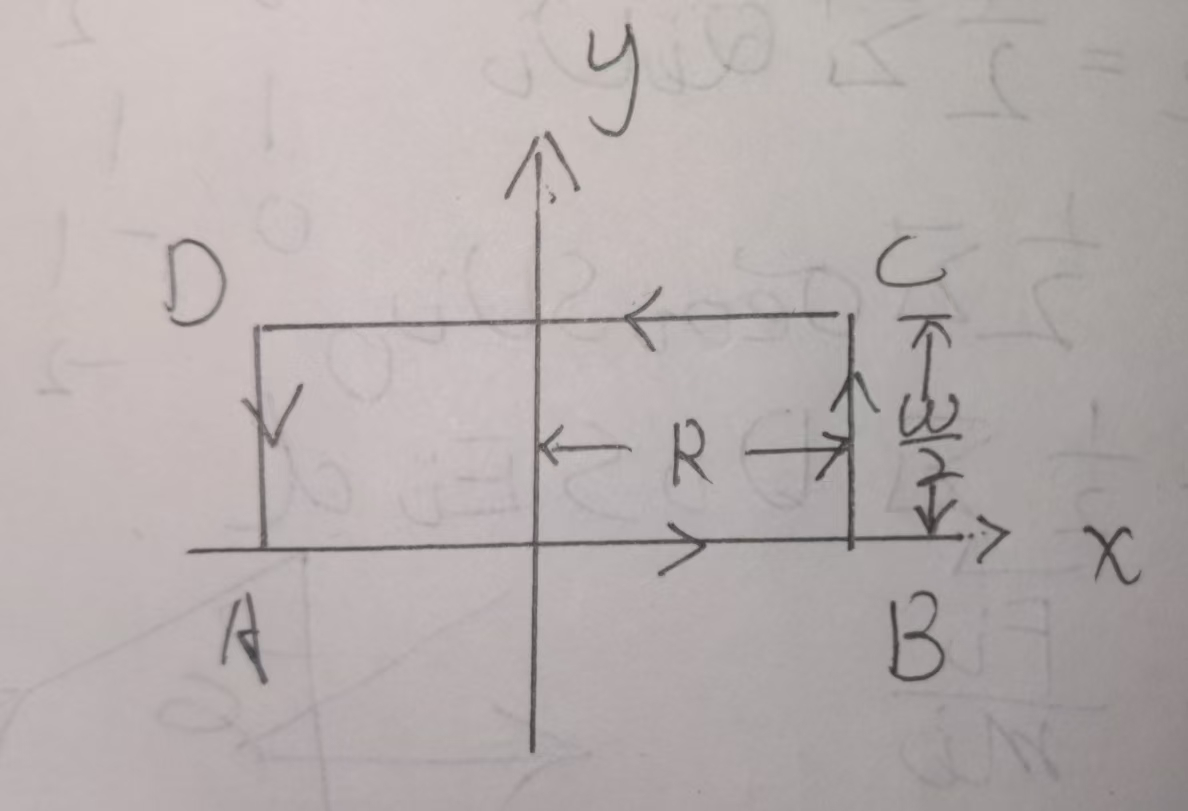
\includegraphics[width=0.7\linewidth]{"picture/lecture 6 积分路径.jpg"}
						\caption{积分路径}
						\label{fig:1}
					\end{figure}
					
					根据柯西积分定理,\(\oint_{L}e^{-z^{2}}dz = 0\)。即:
					% 修正了重复的积分项
					\[\int_{-R}^{R}e^{-x^2}dx + \int_{R}^{R+i\omega/2}e^{-z^2}dz + \int_{R+i\omega/2}^{-R+i\omega/2}e^{-z^2}dz + \int_{-R+i\omega/2}^{-R}e^{-z^2}dz = 0 \]
					
					\begin{itemize}
						\item[(i)] 第一项:当 \(R \to \infty\) 时,\(\int_{-R}^{R}e^{-x^{2}}dx \to \int_{-\infty}^{\infty}e^{-x^{2}}dx = \sqrt{\pi}\)。
						
						\item[(ii)] 第二项(右侧竖直边):令 \( z = R + iy \),其中 \(y\) 从 \(0\) 到 \(\omega/2\)。
						\[
						\left|\int_{0}^{\omega/2}e^{-(R+iy)^{2}}i dy\right| = \left|\int_{0}^{\omega/2}e^{-R^2+y^2-2iRy}i dy\right| \leq \int_{0}^{\omega/2}e^{-R^2+y^2}dy 
						\]
						当 \(R \to \infty\) 时,\(e^{-R^2}\) 趋于0的速度远快于 \(e^{y^2}\) 的增长,故此项积分为 0。
						
						\item[(iii)] 第四项(左侧竖直边):同理,当 \(R \to \infty\) 时,此项积分也为 0。
						
						\item[(iv)] 于是,当 \(R \to \infty\) 时,我们有:
						\[ \int_{-\infty}^{\infty}e^{-x^2}dx + \int_{\infty}^{-\infty}e^{-(x+i\omega/2)^2}dx = 0 \]
						\[ \sqrt{\pi} - \int_{-\infty}^{\infty}e^{-(x+i\omega/2)^2}dx = 0 \]
						这表明 \(\int_{-\infty + i\omega/2}^{\infty + i\omega/2}e^{-z^{2}}dz = \sqrt{\pi}\)。
						
						\item[(v)] 最终:
						\[
						\mathcal{F}(e^{-x^{2}})(\omega) = \frac{1}{\sqrt{2\pi}}e^{-\frac{\omega^{2}}{4}} \cdot \sqrt{\pi} = \frac{1}{\sqrt{2}}e^{-\frac{\omega^{2}}{4}}
						\]
					\end{itemize}
				\end{example}
				
			}
		
			\part{Lecture 10 DFT和FTT}{
				\chapter{DFT}{
					\section{信号}
					$\{x_k: k=0,\dots,N-1\}$,记 $\omega_N = e^{+2\pi i / N}$,其中$z^n=1$
					\begin{equation}
						y_k = \frac{1}{N} \sum_{n=0}^{N-1} x_n e^{-2\pi i \frac{nk}{N}} = \frac{1}{N} \sum_{n=0}^{N-1} x_n \omega_N^{-nk}
					\end{equation}
					称 $\{y_0,\dots,y_{N-1}\}$ 为 $\{x_0,\dots,x_{N-1}\}$ 的 DFT,记 \[\mathcal{F}_N: \C^N \rightarrow \C^N,\quad \mathcal{F}_N(x) = y\]\begin{center}
						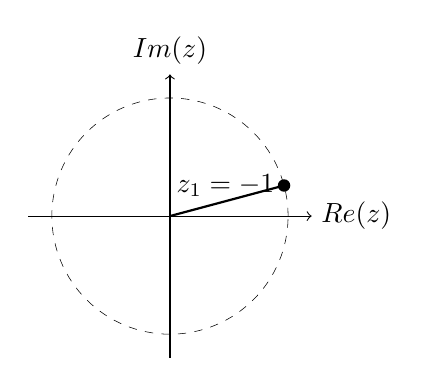
\begin{tikzpicture}[scale = 1.5]
							% 绘制单位圆(虚线)
							\draw[very thin, dashed] (0,0) circle (1cm);
							% 绘制坐标轴
							\draw[->] (-1.2,0) -- (1.2,0) node[right] {$Re(z)$};
							\draw[->] (0,-1.2) -- (0,1.2) node[above] {$Im(z)$};
							
							% 计算并绘制第二个根(k = 1, n = 2)
							\coordinate (root2) at (0.9659,0.25881);
							\draw[thick] (0,0) -- (root2);
							\fill (root2) circle (1.5pt) node[left] {$z_1 = -1$};
						\end{tikzpicture}
					\end{center}
					\section{ 逆公式}
					\begin{lemma}
						\begin{equation}
							x_k = \sum_{n=0}^{N-1} y_n e^{2\pi i \frac{nk}{N}} = \sum_{n=0}^{N-1} y_n \omega_N^{nk}, \text{即} \mathcal{F}_N^{-1}(y) = x.
						\end{equation}
					\end{lemma}
					
					\begin{proof}
						\begin{equation}
							\begin{aligned}
								\sum_{n=0}^{N-1} y_n \omega_N^{nk} 
								&= \sum_{n=0}^{N-1} \left( \frac{1}{N} \sum_{r=0}^{N-1} x_r \omega_N^{-rn} \right) \omega_N^{nk} \\[8pt]
								&= \sum_{r=0}^{N-1} x_r \frac{1}{N} \sum_{n=0}^{N-1} \omega_N^{n(k - r)} \\[8pt]
								&= \sum_{r=0}^{N-1} x_r \delta_{k,r} = x_k.
							\end{aligned}
						\end{equation}
						定义Kronecker-$\delta$函数:
						\begin{equation}
							\delta_{k,r} = 
							\begin{cases} 
								1, & k = r \\[8pt]
								0, & k \neq r 
							\end{cases}
						\end{equation}
						于是
						\begin{equation}
							\frac{1}{N}\sum_{n=0}^{N-1}\omega_N^{n(k-r)}=\delta_{k,r}
						\end{equation}
						
						\begin{itemize}
							\item[(i)]当 $k=r$ 时,显然成立。
							\item[(ii)]当 $k \neq r$ 时
							\begin{equation}
								\begin{aligned}
									\frac{1}{N}\sum_{n=0}^{N-1}\omega_N^{n(k-r)} &= \frac{1}{N} \cdot \frac{1 - \omega_N^{N(k-r)}}{1 - \omega_N^{k-r}} \cdot \omega_N^{k-r} \\[8pt]
									&= \frac{1}{N} \cdot \frac{1 - \omega_N^{N(k-r)}}{1 - \omega_N^{k-r}} \\[8pt]
									&= \frac{1}{N} \cdot \frac{1 - (\omega_N^N)^{k-r}}{1 - \omega_N^{k-r}} = 0(\omega_N^N = 1)
								\end{aligned}
							\end{equation}
						\end{itemize}	
					\end{proof}
					\section{Fourier矩阵}
					\begin{definition}
						定义矩阵$F_N$
						\[F_N=\\ \left( \omega_N^{-nk} \right)_{n,k=0}^{N-1}
						=\begin{bmatrix}
							1 & 1 & 1 & \cdots & 1 \\
							1 & \omega_N & \omega_N^2 & \cdots & \omega_N^{N-1} \\
							1 & \omega_N^2 & \omega_N^4 & \cdots & \omega_N^{2(N-1)} \\
							\vdots & \vdots & \vdots & \ddots & \vdots \\
							1 & \omega_N^{N-1} & \omega_N^{2(N-1)} & \cdots & \omega_N^{(N-1)^2}
						\end{bmatrix}\]
						
						
					\end{definition}
					考虑变换:\[
					\begin{bmatrix}
						y_0 \\
						y_1 \\
						\vdots \\
						y_{N-1}
					\end{bmatrix}
					= F_N
					\begin{bmatrix}
						x_0 \\
						x_1 \\
						\vdots \\
						x_{N-1}
					\end{bmatrix},\]
					\subsection{性质}
					\begin{itemize}
						\item [(i)]
						$F_N$是酉矩阵,$F_N^* F_N = N I_{N \times N}$
						
						\begin{proof}
							第$j$行$(\omega_N^{j \times 0}, \omega_N^{j \times 1}, \omega_N^{j \times 2}, \ldots, \omega_N^{j(N-1)}) \equiv J$
							第$k$行$(\omega_N^{k \times 0}, \omega_N^{k \times 1}, \omega_N^{k \times 2}, \ldots, \omega_N^{k(N-1)}) \equiv K$
							\begin{equation}
								\begin{aligned}
									J^T \overline{K} &= \omega_N^{j \times 0} \overline{\omega_N^{k \times 0}} + \omega_N^{j \times 1} \overline{\omega_N^{k \times 1}} + \cdots + \omega_N^{j(N-1)} \overline{\omega_N^{k(N-1)}} \\[8pt]
									&= \omega_N^{(j - k) \times 0} + \omega_N^{(j - k) \times 1} + \cdots + \omega_N^{(j - k)(N-1)} \\[8pt]
									&= \sum_{m=0}^{N-1} \omega_N^{(j - k)m} = \frac{1 - \omega_N^{(j - k)N}}{1 - \omega_N^{j - k}} = 0(\omega_N^N = 1)
								\end{aligned}
							\end{equation}
						\end{proof}
						\item [(ii)]不同行正交
						\begin{proof}同一行(列)的内积为$N$。
							
							\begin{equation}
								\begin{aligned}
									J^T \overline{J} &= \omega_N^{j \times 0} \overline{\omega_N^{j \times 0}} + \omega_N^{j \times 1} \overline{\omega_N^{j \times 1}} + \cdots + \omega_N^{j(N-1)} \overline{\omega_N^{j(N-1)}} \\[8pt]
									&= 1 + \cdots + 1 = N.
								\end{aligned}
							\end{equation}
						\end{proof}
						\item [(iii)]不同列正交\\
						由上同理可得
						\item [(iv)]$F_N^{-1} = \frac{1}{N} F_N^* = \left( \omega_N^{n\times k} \right)$
					\end{itemize}
					
					
					\section{ 二进制形式下的Fourier矩阵 ($N=2^p$)}
					
					\begin{equation}
						F_2 = \begin{pmatrix} 1 & 1 \\ 1 & \omega_2^{-1 \times 1} \end{pmatrix}
						= \begin{pmatrix} 1 & 1 \\ 1 & e^{-i \frac{2\pi}{2}} \end{pmatrix}
						= \begin{pmatrix} 1 & 1 \\ 1 & -1 \end{pmatrix}
					\end{equation}
					
					\begin{equation}
						\left\{
						\begin{aligned}
							y_0 &= \frac{1}{2}(x_0 + x_1 \omega_2^{-0 \times 1}) \\[8pt]
							y_1 &= \frac{1}{2}(x_0 + x_1 \omega_2^{-1 \times 1})
						\end{aligned}
						\right.
						\Leftrightarrow
						\begin{pmatrix} y_0 \\ y_1 \end{pmatrix}
						= \frac{1}{2} F_2 \begin{pmatrix} x_0 \\ x_1 \end{pmatrix}
						= \begin{pmatrix} \frac{1}{2}(x_0 + x_1) \\ \frac{1}{2}(x_0 - x_1) \end{pmatrix}
					\end{equation}
					
					\begin{table}[h]
						\centering
						\caption{计算量}
						\begin{tabular}{|l|l|}
							\hline
							\textbf{total cost} & \textbf{矩阵计算} \\ \hline
							乘法次数 (multiplications): 0次 & 矩阵及计算: Add $2^1$ \\
							加法次数 (additions): 2次 & multi $2^2$ \\ \hline
						\end{tabular}
					\end{table}
					
					\begin{equation}
						F_4 = \begin{pmatrix}
							1 & 1 & 1 & 1 \\
							1 & \omega_4^{-1 \times 1} & \omega_4^{-2 \times 1} & \omega_4^{-3 \times 1} \\
							1 & \omega_4^{-1 \times 2} & \omega_4^{-2 \times 2} & \omega_4^{-3 \times 2} \\
							1 & \omega_4^{-1 \times 3} & \omega_4^{-2 \times 3} & \omega_4^{-3 \times 3}
						\end{pmatrix}
						=
						\begin{pmatrix}
							1 & 1 & 1 & 1 \\
							1 & -i & -1 & i \\
							1 & -1 & 1 & -1 \\
							1 & i & -1 & -i
						\end{pmatrix}
					\end{equation}
					
					\begin{equation}
						\omega_4 = e^{\frac{2\pi i}{4}} = i,
					\end{equation}
					
					\subsection{ DFT的计算量 (cost of computation)}
					
					\begin{equation}
						y_k = \frac{1}{N} \sum_{n=0}^{N-1} x_n \omega_N^{-nk}
					\end{equation}
					
					每个$y_k$需要$(N-1)$个乘法,$N$个加法。
					
					总乘法次数:$(N-1)^2$
					
					总加法次数:$N(N-1)$
					计算$y_k$时不需要乘法,故不是$N^2$\\用矩阵形式$y = F_N x$理解时,乘法次数为$N^2$;计算复杂度:$O(N^2)$!
				}
				\chapter{FFT}{
					1965年,Cooley和Tukey提出FFT算法。(An algorithm for the machine calculation of complex Fourier series. Mathematics of Computation 19(90): 297-301, Jan 1965.
					DOI: 10.1090/S0025-5718-1965-0178586-1)	
					\section{ FFT ($N=2^2=4$)}
					观察到数据量N=2d以及$(\omega_{2^d})^2=\omega_{ \frac{2^d}{2}}$定义
					\begin{equation}
						F_4: \{x_0, x_1, x_2, x_3\} \rightarrow \{y_0, y_1, y_2, y_3\}
					\end{equation}
					
					\begin{equation}
						y_k = \frac{1}{4} \left( x_0 \omega_4^{-0 \times k} + x_1 \omega_4^{-1 \times k} + x_2 \omega_4^{-2 \times k} + x_3 \omega_4^{-3 \times k} \right), \quad k = 0, 1, 2, 3
					\end{equation}
					
					奇偶重排 (rearrange)可知:
					
					\begin{equation}
						\begin{aligned}
							y_k&=\frac{1}{4}(x_0\cdot w_4^{-0\times k}+x_2 w_4^{-2\times k})+\frac{1}{4}(x_1 w_4^{-1\times k}+x_3 w_4^{-3\times k})\\
							&=\frac{1}{4}(x_0\cdot w_4^{-0\times k}+x_2 w_4^{-2\times k})+\frac{1}{4}w_4^{-1\times k}(x_1 + x_3 w_4^{-2\times k})\\
							&=\frac{1}{4}(x_0 w_2^{-0\times k}+x_2 w_2^{-2\times k})+\frac{1}{4}w_4^{-1\times k}(x_1 + x_3 w_2^{-2\times k})\\
							&=\frac{1}{2}\left[\frac{x_0 + x_2 w_2^{-2\times k}}{2}+\frac{x_1 + x_3 w_2^{-2\times k}}{2}\cdot w_4^{-k}\right]\\
							&\triangleq\frac{1}{2}[P_k + w_4^{-k}I_k]
						\end{aligned}
					\end{equation}
					
					
					\begin{equation}
						P_k = \frac{x_0 + x_2 \omega_2^{-k}}{2}, \quad I_k = \frac{x_1 + x_3 \omega_2^{-k}}{2}, \quad k = 0, 1, 2, 3.
					\end{equation}
					显然:
					\begin{equation}
						P_{k+2} = P_k, \quad k = 0, 1 \quad \text{和} \quad I_{k+2} = I_k, \quad k = 0, 1.
					\end{equation}
					且
					\begin{equation}
						\begin{pmatrix} P_0 \\ P_1 \end{pmatrix} = F_2 \begin{pmatrix} x_0 \\ x_2 \end{pmatrix}, \quad \begin{pmatrix} I_0 \\ I_1 \end{pmatrix} = F_2 \begin{pmatrix} x_1 \\ x_3 \end{pmatrix}
					\end{equation}
					
					则:
					
					\begin{equation}
						\left\{
						\begin{aligned}
							y_k &= \frac{1}{2} \left( P_k + \omega_4^{-k} I_k \right), \quad k = 0, 1 \\[8pt]
							y_{k+2} &= \frac{1}{2} \left( P_{k+2} + \omega_4^{-(k+2)} I_{k+2} \right) = \frac{1}{2} \left( P_k - \omega_4^{-k} I_k \right), \quad k = 0, 1
						\end{aligned}
						\right.
					\end{equation}
					
					至此,$\{ y_0, y_1, y_2, y_3 \}$ 全部算出。
					
					\begin{table}[h]
						\centering
						\begin{tabular}{cccc}
							\toprule
							\textbf{变量} & \textbf{乘法次数} & \textbf{加法次数} & \textbf{备注} \\
							\midrule
							$P_k$ ($k = 0, 1$) & 0次 & 2次 &  \\
							$I_k$ ($k = 0, 1$) & 0次 & 2次 &  \\
							$y_k$ ($k = 0, 1$) & 1次 & 2次 &  \\
							$y_{k + 2}$ ($k = 0, 1$) & 1次 & 2次 & 乘法计算量与$y_k$相同 \\
							\midrule
							\multicolumn{2}{c}{\textbf{优化的总计算量}} & \textbf{乘法1次} & \textbf{加法8次} \\
							\midrule
							\multicolumn{2}{c}{\textbf{直接计算}} & \textbf{乘法9次} & \textbf{加法12次} \\
							\bottomrule
						\end{tabular}
						\caption{计算量对比表}
					\end{table}
					
					计算 $\{y_0, y_1,y_2, y_3\}$ 过程中的计算量:乘法 $1$ 次(表面上 $2$ 次),加法 $8$ 次
					
					对比直接按公式计算的计算量:乘法 $(4-1)^2=9$,加法 $4 \times (4-1)=12$ 次
					\section{ $FFT (N=2^3=8)$}
					
					\begin{equation}
						F_8: \{x_0, x_1, x_2, x_3, x_4, x_5, x_6, x_7\} \rightarrow \{y_0, y_1, \ldots, y_7\}
					\end{equation}
					
					\subsection{递推公式}
					\begin{equation}
						\begin{aligned}
							y_j &= \frac{1}{8} \left( x_0 + x_1 \omega_8^{-1 \times j} + x_2 \omega_8^{-2 \times j} + \cdots + x_6 \omega_8^{-6 \times j} + x_7 \omega_8^{-7 \times j} \right) \\[8pt]
							&= \frac{1}{2} \left( \frac{1}{4} \left( x_0 + x_2 \omega_8^{2 \times j} + x_4 \omega_8^{4 \times j} + x_6 \omega_8^{-6 \times j} \right) \right. \\[8pt]
							&\quad \left. + \frac{1}{4} \left( x_1 \omega_8^{- \times j} + x_3 \omega_8^{-3 \times j} + x_5 \omega_8^{-5 \times j} + x_7 \omega_8^{-7 \times j} \right) \right) \\[8pt]
							&= \frac{1}{2} \left( \frac{1}{4} \left( x_0 + x_2 \omega_4^{- 1\times j} + x_4 \omega_4^{-2\times j} + x_6 \omega_4^{-6 \times j} \right. \right. \\[8pt]
							&\quad \left. \left. + x_1 + x_3 \omega_4^{-1 \times j} + x_5 \omega_4^{-2 \times j} + x_7 \omega_4^{-3 \times j} \right) \omega_8^{-j} \right) \\[8pt]
							&= \frac{1}{2} \left( P_j^{(3)} + I_j^{(3)} \omega_8^{j} \right)
						\end{aligned}
					\end{equation}
					
					
					其中:
					\begin{equation}
						P_j^{(3)} = \frac{1}{4} \left( x_0 + x_2 \omega_4^{-2 \times j} + x_4 \omega_4^{-2\times j} + x_6 \omega_4^{-3 \times j} \right)
					\end{equation}
					
					\begin{equation}
						I_j^{(3)} = \frac{1}{4} \left( x_1 + x_3 \omega_4^{-1 \times j} + x_5 \omega_4^{-2 \times j} + x_7 \omega_4^{-3 \times j} \right)
					\end{equation}
					
					可证:
					\begin{equation}
						\begin{cases}
							P_j^{(3)} = P_{j+4}^{(3)}, \quad j = 0, 1, 2, 3 \\[8pt]
							I_j^{(3)} = I_{j+4}^{(3)}
						\end{cases}
					\end{equation}
					
					\subsection{计算复杂度分析}
					
					\subsubsection{第三层 (A)}
					
					
					$	\text{已知 } P_{j}^{(3)}, I_{j}^{(3)} (j=0,1,2,3), \text{ 计算 } P_{j}^{(3)} (j=0,1,2,3) \text{ 的计算量}$
					
					
					\begin{itemize}
						\item[(i)] 乘法 3 次 (当 $j=0$ 时无乘法)
						\item[(ii)] 加法 8 次
					\end{itemize}
					
					\subsubsection{第二层 (B)}
					$\text{下面讨论 } P_{j}^{(3)} \text{ 的计算量 (} j=0,1,2,3 \text{)}$
					一方面
					\begin{equation}
						\begin{aligned}
							P_{j}^{(3)} &= \frac{1}{4} \left( x_{0}, x_{2}, x_{4}, x_{6} \right) \cdot (1, w_{4}^{-j}, w_{4}^{-2j}, w_{4}^{-3j}) = \text{DFT} \left( x_{0}, x_{2}, x_{4}, x_{6} \right) \\[8pt]
							&= \frac{1}{2} \left\{ \frac{1}{2} \left( x_{0} + x_{4} w_{4}^{-2j} \right) + \frac{1}{2} \left( x_{2} + x_{6} w_{4}^{-j} \right) w_{4}^{-j} \right\} \\[8pt]
							&= \frac{1}{2} \left\{ P_{j}^{(2)} + I_{j}^{(2)} w_{4}^{-j} \right\} \\
							&\quad ( \text{同样地有 } I_{j}^{(3)} = P_{j}^{(2)} + I_{j}^{(2)} w_{4}^{-j} \ \ I_j^{(2)}=I_{j+2} ^{(2)}\quad j=0,1 )
						\end{aligned}
					\end{equation}
					
					如果已知 $P_{j}^{(2)}, I_{j}^{(2)}, j=0,1,2,3$,计算 $P_{j}^{(3)}$ 需要 1 次乘法,4 次加法。
					
					同样地
					\begin{equation}
						\begin{aligned}
							I_{j}^{(3)} &= \frac{1}{4} \left( x_{1}, x_{3}, x_{5}, x_{7} \right) \cdot (1, w_{4}^{-j}, w_{4}^{-2j}, w_{4}^{-3j}) \quad (j=0,1,2,3) \\[8pt]
							&=DFT(x_1,x_3,x_5,x_7)\\[8pt]
							&= \frac{1}{2} \left\{ \frac{1}{2} \left( x_{1} + x_{5} w_{4}^{-2j} \right) + \frac{1}{2} \left( x_{3} + x_{7} w_{4}^{-2j} \right) w_{4}^{-j} \right\} \\[8pt]
							&= \frac{1}{2} \left\{ P_{j}^{(2)} + I_{j}^{(2)} w_{4}^{-j} \right\} \quad (j=0,1)
						\end{aligned}
					\end{equation}
					
					\subsubsection{三层 (C)}
					
					计算 $P_{j}^{(2)}, I_{j}^{(2)}, P_{j}^{(2)}, I_{j}^{(2)}$ ( $j=0,1$ ) 分别需要 0 次乘法,2 次加法。\\
					归纳起来:(A)、(B)、(C) 三层共花费:乘法 3 + 2 + 0 = 5 \quad 加法 8 + 8 + 6 = 24\\
					直接计算时,乘法 $(9-1)= 12$ 次,加法 $8 \times 7 = 56$ 次
					\subsection{FFT ($N = 2^8$, general case)}
					
					\subsection{定义和基本公式}
					\begin{definition}
						\begin{equation}
							F_{2^q}: \mathbb{C}^{2^q} \rightarrow \mathbb{C}^{2^q}
						\end{equation}
					\end{definition}
					\begin{equation}
						(x_0, x_1, \ldots, x_{2^q -1}) \rightarrow (y_0, y_1, \ldots, y_{2^q -1})
					\end{equation}
					\begin{center}
						\begin{equation}
							\begin{aligned}
								y_k &= \frac{1}{2^q} (x_0, x_1, \ldots, x_{2^q -1}) \cdot \left(1, w_{2^q}^{-k}, w_{2^q}^{-2k}, \ldots, w_{2^q}^{-(2^q -1)k}\right)\\
								&= \frac{1}{2^q} \sum_{j=0}^{2^q -1} x_j \left(w_{2^q}\right)^{-jk}, \quad k = 0, 1, \ldots, 2^q -1\\
								&\stackrel{\text{奇偶求和}}{=}  \frac{1}{2} \left\{ \frac{1}{2^{q-1}} \sum_{j=0}^{2^{q-1} -1} x_{2j} \left(w_{2^{q }}\right)^{-2jk} + \frac{1}{2^{q-1}}  \left(w_{2^q}\right)^{-k}\sum_{j=0}^{2^{q-1} -1} x_{2j+1} \left(w_{2^{q }}\right)^{-2jk} \right\}\\
								&=\frac{1}{2} \left\{ \frac{1}{2^{q-1}} \sum_{j=0}^{2^{q-1} -1} x_{2j} \left(w_{2^{q-1}}\right)^{-jk} + \frac{1}{2^{q-1}}  \left(w_{2^q}\right)^{-k}\sum_{j=0}^{2^{q-1} -1} x_{2j+1} \left(w_{2^{q-1}}\right)^{-jk} \right\}\\
								&= \frac{1}{2} \left( P_k^{(q-1)} + w_{2^q}^{-k} I_k^{(q-1)} \right), \quad k = 0, 1, \ldots, 2^{q} -1
							\end{aligned}
						\end{equation}
					\end{center}
					其中:
					\begin{equation}
						P_k^{(q-1)} = \frac{1}{2^{q-1}} \sum_{j=0}^{2^{q-1} -1} x_{2j} \left(w_{2^{q-1}}\right)^{-jk}, \quad k = 0, 1, \ldots, 2^{q-1} -1
					\end{equation}
					
					\begin{equation}
						I_k^{(q-1)} = \frac{1}{2^{q-1}} \sum_{j=0}^{2^{q-1} -1} x_{2j+1} \left(w_{2^{q-1}}\right)^{-jk}, \quad k = 0, 1, \ldots, 2^{q-1} -1
					\end{equation}
					
					利用 $\left(w_{2^q}\right)^{-(k + 2^{q-1})} = -\left(w_{2^q}\right)^k$,得到:
					
					\begin{equation}
						\left\{
						\begin{aligned}
							P_{k + 2^{q-1}}^{(q-1)} &= P_k^{(q-1)} \\[8pt]
							I_{k + 2^{q-1}}^{(q-1)} &= I_k^{(q-1)}
						\end{aligned}
						\right.
						\quad k = 0, 1, \ldots, 2^{q-1} -1
					\end{equation}
					
					因此有公式:
					\begin{equation}
						\left\{
						\begin{aligned}
							y_k &= \frac{1}{2} \left[ P_k^{(q-1)} + \left(w_{2^q}\right)^{-k} I_k^{(q-1)} \right], \quad k = 0, 1, \ldots, 2^{q-1} -1 \\[8pt]
							y_{k + 2^{q-1}} &= \frac{1}{2} \left[ P_k^{(q-1)} - \left(w_{2^q}\right)^{-k} I_k^{(q-1)} \right], \quad k = 0, 1, \ldots, 2^{q-1} -1
						\end{aligned}
						\right.
					\end{equation}
					
					特别地:
					\begin{equation}
						P_k^{(q-1)} = \text{DFT} \left\{ x_{2j} \right\}_{j=0}^{2^{q-1} -1}, \quad k = 0, 1, \ldots, 2^{q-1} -1
					\end{equation}
					
					\begin{equation}
						I_k^{(q-1)} = \text{DFT} \left\{ x_{2j+1} \right\}_{j=0}^{2^{q-1} -1}, \quad k = 0, 1, \ldots, 2^{q-1} -1
					\end{equation}
					
					故有:
					\begin{equation}
						\left\{
						\begin{aligned}
							P_k^{(q-1)} &= P_k^{(q-2)} + \left(w_{2^{q-1}}\right)^{-k} I_k^{(q-2)} \\[8pt]
							I_k^{(q-1)} &= P_k^{(q-2)} + \left(w_{2^{q-1}}\right)^{-k} I_k^{(q-2)}
						\end{aligned}
						\right.
						\quad k = 0, 1, \ldots, 2^{q-2} -1
					\end{equation}
					
					\subsection{FFT 算法中乘法和加法次数的计算}
					记\begin{itemize}
						\item[(1)] \(M_q\):在FFT算法中乘法数(当数据长度为 \(N = 2^q\) 时)\\
						\item[(2)]\(A_q\):在FFT算法中加法数。
					\end{itemize} 已知
					\begin{minipage}[t]{0.45\textwidth}
						\[
						\begin{cases}
							M_1 = 0 \\
							M_2 = 1 \\
							M_3 = 5
						\end{cases}
						\]
					\end{minipage}
					\hfill
					\vrule width 0.4pt
					\begin{minipage}[t]{0.45\textwidth}
						\[
						\begin{cases}
							A_1 = 2 \\
							A_2 = 8 \\
							A_3 = 24
						\end{cases}
						\]
					\end{minipage}
					下面计算 \(M_q\) 与 \(A_q\),首先讨论 \(M_q\) 与 \(M_{q - 1}\) 的关系以及 \(A_q\) 与 \(A_{q - 1}\) 关系:
					\begin{minipage}[t]{0.45\textwidth}
						\begin{center}
							由$A_2$计算 \(P_k^{(q - 1)}\)(DFT of even)\\
							乘法 \(M_{q - 1}\)\\
							计算 \(I_k^{(q - 1)}\)
							\\乘法 \(M_{q - 1}\)
							由公式(乘以 \(w_{2^q}^{k}\))
							\\ 乘法数 \(2^{q - 1} - 1\)
						\end{center}
					\end{minipage}
					\hfill
					\vrule width 0.4pt
					\hfill
					\begin{minipage}[t]{0.45\textwidth}
						加法数 \(A_{q - 1}\)\\
						
						加法数 \(A_{q - 1}\)\\
						
						加法数 \(2^q\)\\
					\end{minipage}
					
					则有:
					\[
					\begin{cases}
						M_q = 2M_{q - 1} + 2^{q - 1} - 1 \\
						M_1 = 0
					\end{cases}
					\quad
					\begin{cases}
						A_q = 2A_{q - 1} + 2^q \\
						A_1 = 2
					\end{cases}
					\]
					\begin{proof}
						\begin{equation}\label{eq:2.3.1}
							\left\{
							\begin{aligned}
								A_q &= 2 A_{q-1} + 2^q  \\[8pt]
								A_1 &= 2
							\end{aligned}
							\right.
						\end{equation}
						
						由\eqref{eq:2.3.1}式知 \(A_{q-j} = 2 A_{q-j-1} + 2^{q-j}\)
						
						则
						\begin{equation}\label{eq:19.2.26}
							2^j A_{q-j} = 2^{j+1} A_{q-j-1} + 2^q 
						\end{equation}
						
						
						令\eqref{eq:19.2.26}中 \(j = 0,1,\ldots,q-2\),然后相加:
						
						\begin{equation}
							\left\{
							\begin{aligned}
								A_q &= 2 A_{q-1} + 2^q \\[8pt]
								2 A_{q-1} &= 2^2 A_{q-2} + 2^q \\[8pt]
								2^2 A_{q-2} &= 2^3 A_{q-3} + 2^q \\[8pt]
								&\vdots \\[8pt]
								2^{q-2} A_2 &= 2^{q-1} A_1 + 2^q
							\end{aligned}
							\right.
						\end{equation}
						由上可得
						\begin{equation}
							A_q = 2^{q-1} A_1 + (q-1) 2^q
						\end{equation}
						则 
						\begin{equation}
							A_q = 2^q + (q-1) 2^q = q 2^q = N \log_2 N
						\end{equation}
						
						因此加法计算量为 \(N \log_2 N = O(N \log N)\)
						
						\begin{equation}\label{eq:19.2.30}
							\left\{
							\begin{aligned}
								M_q &= 2 M_{q-1} + 2^{q-1} -1 \\[8pt]
								M_1 &= 0
							\end{aligned}
							\right.
						\end{equation}
						由\eqref{eq:19.2.30}式知 
						\begin{equation}
							M_{q-j} = 2 M_{q-j-1} + 2^{q -j -1} -1, \quad j=0,1,\ldots,q-2
						\end{equation}
						则
						\begin{equation} 
							2^j M_{q-j} = 2^{j+1} M_{q-j-1} + 2^{q-1} - 2^j
						\end{equation}
						\[
						\begin{cases}
							M_{q} = 2M_{q - 1} + 2^{q - 1} - 1 \\
							2M_{q - 1} = 2^{2}M_{q - 2} + 2^{q - 1} - 2^{1} \\
							2^{2}M_{q - 2} = 2^{3}M_{q - 3} + 2^{q - 1} - 2^{2} \\
							\vdots \\
							2^{q - 2}M_{2} = 2^{q - 1}M_{1} + 2^{q - 1} - 2^{q - 2}
						\end{cases}
						\]
						\[
						\begin{aligned}
							M_{q}&=2^{q - 1}M_{1}+(q - 1)2^{q - 1}-\sum_{j = 0}^{q - 2}2^{j}\\
							&=(q - 1)2^{q - 1}-\frac{1 - 2^{q - 1}}{1 - 2}\\
							&=(q - 1)2^{q - 1}+1 - 2^{q - 1}\\
							&=(q - 2)2^{q - 1}+1\\
							&=\mathcal{O}(N\log_{2}N)
						\end{aligned}
						\]
						
					\end{proof}
				}
			}
			\part{Lecture 11 一元Fourier 变换应用}
			{
				\chapter{微分方程的求解(ordinary)}
				{\textbf{工具:}
					\begin{equation}
						\mathcal{F} D^\alpha = (i \omega)^\alpha \mathcal{F}, 
					\end{equation}
					只有一个维度时:
					\[	(f')^\wedge(\omega) = (i \omega) \hat{f}(\omega) \]
					\(D^\alpha = D_1^{\alpha_1} D_2^{\alpha_2} \cdots D_n^{\alpha_n}\),\(D_j = \frac{\partial}{\partial x_j}\),\(X = (x_1, \ldots, x_n)\),\(X^\alpha = x_1^{\alpha_1} \cdots x_n^{\alpha_n}\)
					\begin{example}
						\begin{equation}
							\int_0^{+\infty} g(w) \sin wt dw = f(t)
						\end{equation}
						求积分方程 的解 \(g(w)\)其中
						\begin{equation}
							f(x) = 
							\begin{cases} 
								\frac{\pi}{2} \frac{\sin(t)}{t}, & 0<t > \pi \\[8pt]
								0, & t \geq \pi
							\end{cases}
						\end{equation}
					\end{example}
					\begin{proof}
						\begin{itemize}
							\item[(i)]
							用正弦变换(略)见书本P69 $\xi$1.6
							\item[(ii)]由于方程中仅仅用到了(0,$\infty$)的的信息,于是$g$在实负半轴可以任意规定
							假设 \(g\) 为奇函数,则:
							\begin{equation}
								\begin{aligned}
									g(w) &= \frac{1}{\sqrt{2 \pi}} \int_{-\infty}^{\infty} \hat{g}(w) e^{-i w t} dw = \frac{1}{\sqrt{2 \pi}} \int_{-\infty}^{\infty} \hat{g}(w) (-i) \sin w t dw \\[8pt]
									&= \frac{-i}{\sqrt{2 \pi}} \int_0^{\infty} g(w) \sin w t dw,
								\end{aligned}
							\end{equation}
							原方程化为:
							\begin{equation}
								\frac{\sqrt{2 \pi}}{-2 i} \hat{g}(t) = f(t)
							\end{equation}
							又 \(g\) 为奇函数,有 \(\hat{g}(-w) = -\hat{g}(w)\)故$f$也做了相应的奇延拓,仍记为 \(f\)
							于是:
							
							\[
							f(t)=\frac{1}{\sqrt{2\pi}}\int_{-\infty}^{\infty} f(w)e^{-iwt}dw=\frac{-2i}{\sqrt{2\pi}}\int_0^{+\infty}f(w)\sin w t dw \]
							\[\qquad=\frac{-2i}{\sqrt{2\pi}}\int_0^\pi \frac{\pi}{2}\sin w t\sin w t dw \]
							\[\qquad=\frac{-2i}{\sqrt{2\pi}}\cdot\frac{\pi}{4}\int_0^\pi [\cos(1-t)w-\cos(1+t)w] dw \]
							\[\qquad=\frac{-2i}{\sqrt{2\pi}}\cdot\frac{\pi}{4}\left( \frac{\sin(1-t)\pi t}{1-t}+\frac{\sin(1+t)\pi t}{1+t} \right) \]
							\[\qquad=\frac{-2i}{\sqrt{2\pi}}\cdot\frac{\pi}{4}\left( \frac{\sin \pi t}{1-t}+\frac{\sin \pi t}{1+t} \right) \]
							\[\qquad=\frac{-2i}{\sqrt{2\pi}}\cdot\frac{\pi}{4}\cdot 2\cdot\frac{\sin\pi t}{1-t^2}=\frac{-2i}{\sqrt{2\pi}}\cdot\frac{\pi}{2}\cdot\frac{\sin \pi t}{1-t^2} \]
							对$\frac{\sqrt{2\pi}}{-2i}\hat{g}(t) = f(t)$两边做傅里叶变换
							\[
							\frac{\sqrt{2\pi}}{-2i} \widehat{\hat{g}(t)} =\hat{f(t)}
							\]
							利用$\mathcal{F}^2=mirror$的性质\[
							\mathcal{F}^{2}\{f(t)\} = \mathcal{F}\{\mathcal{F}\{f(t)\}\} = f(-t)\]
							而且\(g\)为奇函数可知
							\[
							\frac{\sqrt{2\pi}}{-2i}g(-t) = \frac{-2i}{\sqrt{2\pi}} \cdot \frac{\pi}{2} \cdot \frac{\sin \pi t}{1 - t^2}
							\]
							\[	g(t) = \frac{\sin\pi t}{1 - t^2}\]	\end{itemize}
					\end{proof}
					\begin{example}
						积分方程解
						\[	g(t) = h(t) + \int_{-\infty}^{\infty} f(t) g(t - x) dx\]
						\( h \)、\( f \) 已知,且 \( g \)、\( h \)、\( f \) 的傅里叶变换存在。	\end{example}
					\begin{proof}
						由傅里叶变换的卷积公式:
						\[	\mathcal{F}\{f * g\} = \sqrt{2\pi} \cdot \hat{f} \cdot \hat{g}
						\]
						原方程可化为:
						\[\hat{g}(w) = \hat{h}(w) + \hat{f}(w) \cdot \hat{g}(w) \cdot \sqrt{2\pi}\]	
						解得:
						\[\hat{g}(w) = \frac{\hat{h}(w)}{1 - \sqrt{2\pi} \cdot \hat{f}(w)}\]
						\[
						g(t) = \frac{1}{\sqrt{2\pi}} \int_{-\infty}^{\infty} \frac{\hat{h}(w)}{1 - \sqrt{2\pi} \cdot \hat{f}(w)} e^{iwt} dw
						\]
					\end{proof}
					\begin{example}
						常微分非齐次线性积分方程:
						\begin{equation}
							y'' - y = -f
						\end{equation}
						其中$ f$为已知函数\end{example}
					\begin{proof}
						对两边取Fourier变换:
						\begin{equation}
							(iw)^2 \hat{y}(w) - \hat{y}(w) = -\hat{f}(w)
						\end{equation}
						
						解得:
						\begin{equation}
							\hat{y}(w) = \frac{\hat{f}(w)}{1 + w^2}
						\end{equation}
						
						因此:
						\begin{equation}
							y(t) = \frac{1}{\sqrt{2\pi}} \int_{-\infty}^{\infty} \frac{\hat{f}(w)}{1 + w^2} e^{iwt} dw
						\end{equation}
						
						将 \(\frac{\hat{f}(w)}{1 + w^2}\) 视为 \(\hat{f}(w)\) 与 \(\frac{1}{1 + w^2}\) 的乘积。
						由卷积定理:
						\begin{equation}
							(f * h)(w) = \sqrt{2\pi} \hat{f}(w) \cdot \hat{h}(w), \quad \text{其中} \, \hat{h}(w) = \frac{1}{1 + w^2}.
						\end{equation}
						因此:
						\begin{equation}
							\hat{y}(w) = \sqrt{2\pi} \hat{f}(w) \cdot \hat{g}(w), \quad \text{其中} \, \hat{g}(w) = \frac{1}{\sqrt{2\pi}} \cdot \frac{1}{1 + w^2}.
						\end{equation}
						所以:
						\begin{equation}
							y(t) = (f * g)(t), \quad \text{其中} \, g(w) = \frac{1}{2} e^{-|t|}.
						\end{equation}
						因此:
						\[	g(t) = \frac{1}{\sqrt{2\pi}} \int_{-\infty}^{\infty} \frac{1}{1 + w^2} e^{iwt} dw=\frac{ 1}{2}e^{-|t|}\]
						
						\begin{equation}
							y(t) = \frac{1}{2} \int_{-\infty}^{\infty} f(t) e^{-|t - x|} dx.
						\end{equation}
					\end{proof}
					\begin{example}
						求解积分方程:
						\begin{equation}
							a x'(t) + b x(t) + c \int_{0}^{t} x(t) dt = h(t),
						\end{equation}
						其中 $ a, b, c \in \mathbb{R}$,  $h  $已知\end{example}
					\begin{proof}
						关键是通过$\mathcal{F}$变换求解。设 \(G' = g\),且 \(G\) 有傅里叶变换。	
						对两边取$\mathcal{F}$:
						\[	(iw) \hat{G}(w) = \hat{g}(w) \Rightarrow \hat{G}(w) = \frac{\hat{g}(w)}{iw}.\]
						利用此公式,原方程可变换为:
						\[	a (iw) \hat{x}(w) + b \hat{x}(w) + c \frac{\hat{x}(w)}{iw} = h(w)\]
						
						解得:
						\[\hat{x}(w) = \frac{h(w)}{iaw + b + \frac{c}{iw}}.\]
						
					\end{proof}
					
					
				}
				
				\chapter{The Solution of Partial Differential Equation by $\mathcal{F}$ }
				{
					\section{一维波动方程初值问题}
					\[\left\{\begin{array}{l}
						
						\large \displaystyle\frac{\partial^2 u}{\partial t^2}= \frac{\partial^2 u}{\partial x^2}, \quad x \in \mathbb{R}, t > 0\\
						\large \displaystyle u|_{t=0}=  \cos(x)\\
						\large \displaystyle \frac{\partial u}{\partial t}\bigg|_{t=0} = \sin(x)
					\end{array}\right.\]
					\begin{proof}
						对二元函数 \(u(x, t)\) 的 \(x\) 变量作偏$\mathcal{F}_1$,记之为 \(V(w, t)\)。则:\[
						V(w, t) = \frac{1}{\sqrt{2\pi}} \int_{-\infty}^{\infty} u(x, t) e^{-iwx} dx\]
						\begin{itemize}
							\item[(I)]
							
							于是:\[
							\frac{\partial V}{\partial t}(w, t)=	\frac{\partial  }{\partial t}\mathcal{F}_1(u(x, t)) =\frac{1}{\sqrt{2\pi}}\frac{\partial }{\partial t} \int_{-\infty}^{\infty} u(x, t) e^{-iwx} dx\] \[=\frac{1}{\sqrt{2\pi}} \int_{-\infty}^{\infty} \frac{\partial u}{\partial t}(x, t) e^{-iwx} dx = \mathcal{F}_1\left( \frac{\partial u}{\partial t}(x, t) \right)\]
							即微分和$\mathcal{F}_1$能够换序
							\[\frac{\partial}{\partial t}(\mathcal{F}_1 u(x, t))=\mathcal{F}_1\left( \frac{\partial u}{\partial t} \right)(w, t)  \]
							同样
							\[\frac{\partial^2}{\partial t^2}(\mathcal{F}_1 u(x, t))=\mathcal{F}_1\left( \frac{\partial^2 u}{\partial t^2} \right)(w, t)  \]
							\[\mathcal{F}_1\left( \frac{\partial u}{\partial t} \right)(w, t) = \frac{\partial}{\partial t} V(w, t) \quad \text{(视 \(w\) 为常数)}\]\[
							\mathcal{F}_1\left( \frac{\partial^2 u}{\partial t^2} \right)(w, t) =  \frac{\partial^2 u}{\partial t^2} V(w, t)\]\[
							\mathcal{F}_1\left( \frac{\partial  u}{\partial x } \right)(w, t) = (iw)  V(w, t)
							\]\[
							\mathcal{F}_1\left( \frac{\partial^2 u}{\partial x^2} \right)(w, t) = (iw)^2 V(w, t)
							\]\[
							\mathcal{F}_1\left( \sin x \right)(w) = \sqrt{\frac{\pi}{2}} i \left[ \delta(w + 1) - \delta(w - 1) \right]\]
							\[		\mathcal{F}_1\left( \cos x \right)(w) = \sqrt{\frac{\pi}{2}} \left[ \delta(w + 1) + \delta(w - 1) \right]\]
							\item [(II)]原方程在频率域可转化为常微分方程问题
							\[
							\left\{ \begin{array}{l}
								\renewcommand{\arraystretch}{2.0} % 增加行距,2.0 是倍数,可以根据需要调整
								\large \displaystyle \frac{ \mathbf{d}^2 V}{\mathbf{d}t^2}= -w^2V   \\[0.5cm] % [0.5cm] 也可以手动增加行距
								\large \displaystyle V|_{t=0}= \sqrt{\frac{\pi}{2}} \left[ \delta(w + 1) + \delta(w - 1) \right] \\[0.5cm]
								\large \displaystyle \frac{\mathbf{d}V}{\mathbf{d}t}|_{t=0} = \sqrt{\frac{\pi}{2}} \cdot i \left[ \delta(w + 1) - \delta(w - 1) \right] 	
							\end{array} \right.
							\]
							\[V(w, t) = C_1 \sin(wt) + C_2 \cos(wt)\]
							齐次方程特征方程为 \(\lambda^2 + w^2 = 0\),其解为 \(\lambda = \pm iw\),对应的解为 \(e^{\pm iwt}\),即 \(\cos(wt)\) 和 \(\sin(wt)\)。
							由第一个边界条件:\[
							C_2 = \sqrt{\frac{\pi}{2}} \left[ \delta(w + 1) + \delta(w - 1) \right]\]
							第二个边界条件:\[	C_1 = \sqrt{\frac{\pi}{2}} \cdot \frac{i}{w} \left[ \delta(w + 1) - \delta(w - 1) \right]\]	
							最后得
							\begin{equation}
								\begin{aligned}
									V(w, t) &= \sqrt{\frac{\pi}{2}} \cdot \frac{i}{w} \left[ \delta(w + 1) - \delta(w - 1) \right] \sin(wt) \\[8pt]
									&\quad + \sqrt{\frac{\pi}{2}} \left[ \delta(w + 1) + \delta(w - 1) \right] \cos(wt) \\[8pt]
									&= \left( \sqrt{\frac{\pi}{2}} \cdot \frac{i}{w} \sin(wt) + \sqrt{\frac{\pi}{2}} \cos(wt) \right) \delta(w + 1) \\[8pt]
									&\quad + \left( -\sqrt{\frac{\pi}{2}} \cdot \frac{i}{w} \sin(wt) + \sqrt{\frac{\pi}{2}} \cos(wt) \right) \delta(w - 1)
								\end{aligned}
							\end{equation}
							做逆变换,频率到时间
							\item[(III)]
							\[	
							u(x, t) = \mathcal{F}_1^{-1}(V(\cdot, t))(x) \]
							\[	= \frac{1}{\sqrt{2\pi}} \int_{-\infty}^{\infty} \left\{ \left[ \sqrt{\frac{\pi}{2}} \cdot \frac{i}{w} \sin(wt) + \sqrt{\frac{\pi}{2}} \cos(wt) \right] \delta(w + 1) \right. \]
							\[\quad \left. + \left[ -\sqrt{\frac{\pi}{2}} \cdot \frac{i}{w} \sin(wt) + \sqrt{\frac{\pi}{2}} \cos(wt) \right] \delta(w - 1) \right\} e^{iwx} dw \]
							\[= \frac{1}{\sqrt{2\pi}} \left\{ \left[ \sqrt{\frac{\pi}{2}} \cdot \frac{i}{-1} \sin(-t) + \sqrt{\frac{\pi}{2}} \cos(-t) \right] e^{-ix} \right. \]
							\[\quad \left. + \left[ \sqrt{\frac{\pi}{2}} \cdot \frac{-i}{1} \sin(t) + \sqrt{\frac{\pi}{2}} \cos(t) \right] e^{ix} \right\} \]
							\[= \frac{1}{2} \left\{ \left[ -i \sin(t) + \cos(t) \right] e^{ ix} + \left[ i \sin(t) + \cos(t) \right] e^{-ix} \right\} \]
							\[= \cos(t - x)\]
							
						\end{itemize}
					\end{proof}
					
					\section{一维热传导问题}
					\[\left\{\begin{array}{l}
						\Large \displaystyle\dfrac{\partial u}{\partial t} = a^2\dfrac{\partial^2 u}{\partial x^2} + f(x,t),  x \in \R, t > 0\\
						\Large \displaystyle 	u|_{t=0}  = \varphi(x) \\	
					\end{array}\right.\]
					\begin{proof}
						\begin{itemize}\item [(1)]
							令 \(V(w,t) = \mathcal{F}_1(u(\cdot,t))(w)\).\[
							则\mathcal{F}_1\left(\frac{\partial u}{\partial t}(\cdot,t)\right) = \frac{\partial}{\partial t}(\mathcal{F}_1 u(w,t)) = \frac{\partial}{\partial t}V(w,t) \stackrel{note}{=} \frac{dV}{dt}(w,t) \]\[
							\mathcal{F}_1\left(\frac{\partial^2 u}{\partial x^2}\right)(w) = (iw)^2 V(w,t) = -w^2 V(w,t) \]记\[
							\hat{f}_1(w,t) = \mathcal{F}_1 f(\cdot,t)(w) \label{eq:fourier_f} \]
							\[\hat{\varphi}(w) = (\mathcal{F}\varphi)(w) \]
							则原方程在频域表示为:
							\[\left\{\begin{array}{l}
								\Large \displaystyle\	\frac{dV}{dt} =-a^2 w^2 V +\hat{f}_1(w,t)\\
								\Large \displaystyle V|_{t=0} = \hat{\varphi}(w) \\
								
							\end{array}\right.\]
							一阶非齐次常微分方程可由常数变易法求解
							\[	V(w, t) = \hat{\varphi}(w) e^{-a^2 
								w^2 t} + \int_0^t \hat{f}_1(w, \tau) e^{-a^2 w^2 (t - \tau)} d\tau \]
							\item [(2)]逆变换:
							利用\[	\mathcal{F}\left(e^{-\frac{(\cdot)^2}{\beta } }\right)(w) = \sqrt{\frac{ \beta}{2}} e^{-\dfrac{\beta w^2}{4}}(\beta=\frac{1}{a^2t} )\]
							\[
							\mathcal{F}^{-1}\left(e^{-a^2 w^2 t}\right)(x) = \sqrt{2\pi} \cdot \dfrac{1}{2a\sqrt{\pi t}} e^{-\dfrac{x^2}{4a^2 t}}\]
							做平移调制\[	\mathcal{F}^{-1}\left(e^{-a^2 (t-x)(\cdot)^2 }\right)(y) = \dfrac{1}{a\sqrt{2\pi (t -x)}} e^{-\dfrac{(y)^2}{4a^2 (t -x)}}\]
							得解:
							\begin{equation}
								\begin{aligned}
									u(x, t) &= \left( \varphi(\cdot) * \dfrac{1}{a\sqrt{2\pi t}} e^{-\dfrac{x^2}{4a^2 t}} \right)(x) \\
									&\quad + \int_0^t \left( f(\cdot, x) * \dfrac{1}{a\sqrt{2\pi (t -  x)}} e^{-\dfrac{(\cdot)^2}{4a^2 (t - x)}} \right)(x) dx
								\end{aligned}
							\end{equation}
						\end{itemize}
					\end{proof}
					
					\section{关于上半平面无源静电场电势的边值问题}
					\[\left\{\begin{array}{l}
						\Large \displaystyle \frac{\partial^2 u}{\partial x^2} + \frac{\partial^2 u}{\partial y^2} = 0,  x \in \mathbb{R}, y > 0\\
						\Large \displaystyle 		u|_{y=0} = f(x) \\	
					\end{array}\right.\]
					\begin{proof}
						记 $V(w, y) = \mathcal{F}_1 u(x, y)(w)$。则原方程转化为
						\[\left\{\begin{array}{l}
							\Large \displaystyle - w^2 V(w, y) +  \frac{\partial^2}{\partial y^2}V(w, y) = 0 \\
							\Large \displaystyle 			V(w, y)|_{y=0} = \hat{f}(w) \\
							\Large \displaystyle	\lim_{y \to +\infty} V(w, y) = 0  
						\end{array}\right.\]
						视 $w$ 为常数,这是一个二阶常微分方程。特征方程为:
						\[
						\lambda^2 - w^2 = 0 \implies \lambda = \pm |w|
						\]
						通解为:
						\[
						V(w, y) = C_1 e^{|w| y} + C_2 e^{-|w| y}
						\]边值条件给出:
						\[
						V(w, y)|_{y=0} = \hat{f}(w) \implies C_1 + C_2 = \hat{f}(w)
						\]
						以及
						\[
						\lim_{y \to +\infty} V(w, y) = 0 \implies C_1 = 0
						\]
						
						因此:
						\[
						V(w, y) = \hat{f}(w) e^{-|w| y}
						\]
						利用Fourier逆变换:
						\[	\mathcal{F}^{-1}\left(e^{-|w| y}\right)(x) = \sqrt{\dfrac{\pi}{y}} \dfrac{y}{x^2 + y^2}
						\]
						上式子可由下式得出
						\[
						\mathcal{F}\left(e^{-\frac{1}{r}}\right)(\xi) \rightleftarrows \sqrt{\dfrac{\pi}{2}} \dfrac{r}{1 + r^2 \xi^2}
						\]最终得解
						\begin{equation}
							\begin{aligned}
								u(x, y) &= \frac{1}{\sqrt{2 \pi}}\left(f * \sqrt{\frac{2}{\pi}} \frac{y}{(\cdot)^{2} + y^{2}}\right)(x) \\
								&= \frac{1}{\pi} \int_{-\infty}^{\infty} \frac{y}{x^{2} + y^{2}} f(x - t) \, dt
							\end{aligned}
						\end{equation}
						副产物:上半平面 Poisson 积分核
						\begin{equation}
							P_y(x) = \dfrac{1}{\pi} \cdot \dfrac{y}{y^2 + x^2}
						\end{equation}	
					\end{proof}
					
				}
				
			}
			\part{Lecture 12 多元Fourier变换}
			{
				
				\chapter{基本定义与性质}
				{
					\begin{definition}
						\[
						\mathcal{F}f(\vec{\omega})= \mathcal{F}f(\omega_1, \dots, \omega_m) \]
						\[= \left(\frac{1}{\sqrt{2\pi}}\right)^m \int _{\mathbb{R}^m}{ f(x_1, \dots, x_m) e^{-i(\omega_1x_1 + \cdots + \omega_mx_m)}  }dx_1 \cdots dx_m \]
						\[= \frac{1}{(2\pi)^{m/2}} \int _{\mathbb{R}^m} f(\vec{x}) e^{-i \vec{\omega} \cdot \vec{x}} d\vec{x}\]
					\end{definition}
					\section{一些工具}
					\subsection{逆公式}
					\[	f(\vec{x}) = \frac{1}{(2\pi)^{m/2}} \int _{\mathbb{R}^m} \hat{f}(\vec{\omega}) e^{i \vec{w} \cdot \vec{x}} d\vec{\omega}\]
					\subsection{偏傅里叶变换}
					\[\mathcal{F}_j f(x_1, \dots, x_{j-1},\omega_j, x_{j+1}, \dots, x_m) = \frac{1}{\sqrt{2\pi}} \int _{-\infty}^{\infty} f(\vec{x}) e^{-i \omega_j x_j}dx_j\]
					当 $f(\vec{x}) = \prod_{j=1}^m g_j(x_j)$ 变量可分离时,则得到张量对角积
					\[(\mathcal{F}f)(\vec{\omega}) = \prod_{j=1}^m \mathcal{F}_j g_j(\omega_j)
					\]
					
					\begin{example}
						求函数 \( f(x) = a e^{-b^2 |x|^2} = a e^{-b^2 (x_1^2 + x_2^2)} \) 的二维傅里叶变换 \( \hat{f}(w_1, w_2) \)。
					\end{example}
					\begin{proof}
						应用二维傅里叶变换公式:
						\[	\hat{f}(w_1, w_2) = \frac{1}{(\sqrt{2\pi})^2} \int_{-\infty}^{\infty} \int_{-\infty}^{\infty} a e^{-b^2 (x_1^2 + x_2^2)} e^{-i(w_1 x_1 + w_2 x_2)} dx_1 dx_2\]
						\[\stackrel{fubini}{=}	\hat{f}(w_1, w_2) = \frac{1}{\sqrt{2\pi}} \left( \int_{-\infty}^{\infty} a e^{-b^2 x_1^2} e^{-i w_1 x_1} dx_1 \right) \left( \frac{1}{\sqrt{2\pi}}\int_{-\infty}^{\infty} e^{-b^2 x_2^2} e^{-i w_2 x_2} dx_2 \right)\]
						利用两者其一\[\mathcal{F}(e^{-\beta (\cdot)^2})(w) = \sqrt{\frac{1}{2\beta}} e^{-\frac{w^2}{4\beta}}\]
						\[	\mathcal{F}(e^{-\frac{\cdot ^2}{\beta}})(w) = \sqrt{\frac{1}{2\beta}} e^{-\beta\frac{w^2}{4}}\]
						\[\hat{f}(w_1, w_2) = \frac{a}{4 b^2} \exp\left(-\frac{w_1^2 + w_2^2}{4 b^2}\right)\]
						特别地,当 \( a = 1 \), \( b = 1 \) 时,结果简化为:
						\begin{equation}
							\hat{f}(w_1, w_2) = \frac{1}{4} \exp\left(-\frac{w_1^2 + w_2^2}{4}\right)
						\end{equation}为算子的不动点。
					\end{proof}
					\begin{example}
						求函数 \( f(x) = e^{-x^{T} A x} \) 的傅里叶变换,其中 \( x = (x_1, \dots, x_m)^{'} \),且 \( A = B^{T} B \)为正定矩阵,B可逆
					\end{example}
					\begin{proof}
						\[	e^{-x^{T} A x} = e^{-x^{T} B^{T} B x} = e^{-(B x)^{T} (B x)}\]	
						\[	\hat{f}(w_1, \dots, w_m) = \frac{1}{(\sqrt{2\pi})^m} \int_{\mathbb{R}^m} e^{-(B x)^{T} (B x)} e^{-i w^{T} x} dx
						\]
						令 \( y = B x \),则 \( x = B^{-1} y \),且雅可比行列式 \( |B^{-1}| \)。代入上式得到:
						\[	\hat{f}(w) = \frac{1}{(\sqrt{2\pi})^m} \int_{\mathbb{R}^m} e^{-y^{T} y} e^{-i \omega^{T} B^{-1} y} \frac{1}{|B|} dy
						\]
						\[= \frac{1}{(\sqrt{2\pi})^m} \int_{\mathbb{R}^m} e^{-|y^2|} e^{-i ({B^{-1}}^{T}\omega)^T y} \frac{1}{|B|} dy\]
						利用:$\mathcal{F}(e^{-|x|^2})(\omega_1,\omega_2,......\omega_m) = \frac{1}{(\sqrt{2 })^m} e^{-\frac{w^T w}{4}}$
						\[\hat{f}(w) = \frac{1}{(\sqrt{2})^m} \frac{1}{|B|} e^{-\frac{(B^{-1} w)^T ((B^{-1})^T w)}{4}}	\]
						\[= \frac{1}{(\sqrt{2})^m} \frac{1}{|B|} e^{-\frac{w^T B^{-1}(B^{-1})^{T}  w}{4}}	\]
						\[ A = B^T B \rightarrow (B^{-1})^T B^{-1} = A^{-1} \]
						\[	\hat{f}(w) = \frac{1}{(\sqrt{2})^m} \frac{1}{|B|} e^{-\frac{w^T A^{-1} w}{4}}	\]
						当 \( B = I \) 时 
						\[
						\hat{f}(w) = \frac{1}{(\sqrt{2})^m} e^{-\frac{w^T w}{4}}
						\]
					\end{proof}
					\section{性质}
					线性性,略
					\subsection{平移性}
					\begin{equation}
						\mathcal{F}(f(x - \vec{a})) = e^{-i \vec{a} \cdot \vec{\omega}} (\mathcal{F}f)(\vec{\omega})
					\end{equation}
					即
					\begin{equation}
						F T_{\vec{a}} = M_{-\vec{a}} F.
					\end{equation}
					
					\subsection{调制性}
					\begin{equation}
						F M_{\vec{b}} = T_{\vec{b}} F.
					\end{equation}
					
					\subsection{微分性质}
					\[\mathcal{F}\left(\dfrac{\partial}{\partial x_j}  \right) = (i w_j) \cdot \mathcal{F} \]
					\[\dfrac{\partial}{\partial w_j} \mathcal{F}f = \mathcal{F}\left(-i x_j f\right)\{\textbf{即}	\dfrac{\partial}{\partial w_j} \hat{f}(\vec{w}) = \mathcal{F}\left(-i x_j f(x)\right)(\vec{w})\}\]
					一般化
					令\(k = (k_1, \dots, k_m)\),\(D = \left(\dfrac{\partial}{\partial x_1}, \dots, \dfrac{\partial}{\partial x_m}\right)\),则:
					\[D^{k} = \dfrac{\partial^{|k|}}{\partial x_1^{k_1} \cdots \partial x_m^{k_m}}(\textbf{其中} |k| = k_1 + \cdots + k_m )。
					\]
					则有:
					\[\mathcal{F}(D^{k} f)(\vec{w}) = \left(i (w_1, \dots, w_m)^{(k_1,k_2,...k_m)}\right) (\mathcal{F}f)(\vec{w})\]
					
					当 \(P_m\) 为 \(m\) 元多项式时:
					\[\mathcal{F}(P_m(D) f)(\vec{w}) = P_m(i \vec{w}) (\mathcal{F}f)(\vec{w})\]
					请回忆多元微分学的多元Taylor公式,特别地:
					\[D^{k} \mathcal{F}f(\vec{w}) = \mathcal{F}((-i x)^{k} f)(\vec{w})\]
					即:\[P_m(D) \mathcal{F}f(\vec{w}) = \mathcal{F}(P_m(-i x) f)(\vec{w})\]
					\subsection{卷积}
					\[
					\mathcal{F}(f * g)(w) = (\sqrt{2\pi})^m (\mathcal{F}f)(w) \cdot(\mathcal{F}g)(w)
					\]\[
					\mathcal{F}(f \cdot g)(w) = (\sqrt{2\pi})^{-m} \left( (\mathcal{F}f) * (\mathcal{F}g) \right)(w)
					\]
					\subsection{多维情况}
					对于多维情况,傅里叶变换具有如下性质:
					\[
					\mathcal{F}\left( f_1 * f_2 * \cdots * f_n \right)(w) = (\sqrt{2\pi})^{m(n-1)} \prod_{j=1}^n (\mathcal{F}f_j)(w)
					\]\[
					\mathcal{F}\{\prod_{j=1}^n (f_j)\}(w) = (\sqrt{2\pi})^{-m(n-1)} (\mathcal{F}f_1*\mathcal{F}f_2\cdots * \mathcal{F}f_n)(w)
					\]
					
					\subsection{缩放}
					\[
					\mathcal{F}\{f(A\cdot \vec{x})\}(w) = |A|^{-\frac{m}{2}} (\mathcal{F}f)(\{A^{-1})^{T} \cdot w^T\}^T )
					\]简要证明:
					\begin{proof}
						注意单位化和$A\cdot\vec{x}$的含义
						\[	\mathcal{F}\{f(A\cdot \vec{x})\}(w)=\frac{1}{(\sqrt{2\pi |{A}|})^m}\int_{\mathbb{R}^m }^{} f(A\cdot \vec{x}) e^{-i\vec{\omega}\cdot\vec{x}}  d\{A\cdot\vec{x}\}\]
						\[\stackrel{\vec{y}=A\cdot \vec{x}}{=}
						\frac{1}{(\sqrt{2\pi|{A}|})^m}\int_{\mathbb{R}^m}^{ } f( \vec{y}) e^{-i\vec{\omega}\cdot A^{-1}\cdot\vec{y}}  d\vec{y}\]
						做转置问题得证
					\end{proof}
				}
				\chapter{多元Fourier变换应用}{
					\section{二维热传导方程的初值问题}
					考虑如下定解问题:
					\[
					\begin{cases}
						\frac{\partial u}{\partial t}=a^{2}\left(\frac{\partial^{2}u}{\partial x^{2}}+\frac{\partial^{2}u}{\partial y^{2}}\right)\\
						\left.u\right|_{t = 0}=\varphi(x,y)
					\end{cases}
					\]
					其中 \((x,y)\in\mathbb{R}^{2}\),\(t>0\)
					\begin{proof}
						\begin{itemize}
							\item[(I)]. “冻结”时间,对三元函数 \(u(x,y,t)\) 关于 \((x,y)\) 变量施加二维傅里叶变换。
							\[V(w_{1},w_{2},t)=\mathcal{F}[u(\cdot,\cdot,t)](w_{1},w_{2})\]
							由 \(\frac{\partial}{\partial t}\) 与 \(\mathcal{F}\) 的可交换性(即 \(\mathcal{F}(\frac{\partial}{\partial t})=\frac{\partial}{\partial t}\mathcal{F}\)),有:
							\[
							\mathcal{F}\left(\frac{\partial u}{\partial t}\right)(w_{1},w_{2},t)=\frac{\partial}{\partial t}(\mathcal{F}u)(w_{1},w_{2},t)=\frac{\partial}{\partial t}V(w_{1},w_{2},t)
							\]\[\begin{cases}
								\mathcal{F}\left(\frac{\partial^{2}u}{\partial x^{2}}\right)(w_{1},w_{2},t)=-w_{1}^{2}V(w_{1},w_{2},t)\\
								\mathcal{F}\left(\frac{\partial^{2}u}{\partial y^{2}}\right)(w_{1},w_{2},t)=-w_{2}^{2}V(w_{1},w_{2},t)\end{cases}\]
							\item[(II)]. 则原初值问题转化为:
							\[
							\begin{cases}
								\frac{d V}{d t}=-a^{2}(w_{1}^{2}+w_{2}^{2})V\\
								\left.V\right|_{t = 0}=\hat{\varphi}(w_{1},w_{2})
							\end{cases}
							\]
							\item[(III)]  常系数ODE \(\frac{dV}{dt}=-a^{2}(w_{1}^{2}+w_{2}^{2})V\) 的通解为:
							\[
							V(w_{1},w_{2},t)=C e^{-a^{2}(w_{1}^{2}+w_{2}^{2})t}
							\]
							\item[(IV)]. 求 \(C\),由初始条件 \(\left.V\right|_{t = 0}=\hat{\varphi}\),可得 \(C = \hat{\varphi}(w_{1},w_{2})\)。
							\item[(V)]. 所以 \(V(w_{1},w_{2},t)=\hat{\varphi}(w_{1},w_{2})e^{-a^{2}t(w_{1}^{2}+w_{2}^{2})}\)。
							利用二维卷积性质 \((\mathcal{F}(f*g)=(\mathcal{F}f)\cdot(\mathcal{F}g))\)
							\[	u(x,y,t)=\mathcal{F}^{-1}[\hat{\varphi}(\cdot,\cdot)]*\mathcal{F}^{-1}[g(\cdot,\cdot,t)]\]其中 \[g(x,y,t)=\mathcal{F}^{-1}\left(e^{-a^{2}t(w_{1}^{2}+w_{2}^{2})}\right)(x,y)\]
							由于变量可分离:\(e^{-a^{2}t(w_{1}^{2}+w_{2}^{2})}=e^{-a^{2}tw_{1}^{2}}\cdot e^{-a^{2}tw_{2}^{2}}\)
							再利用一元$\mathcal{F}$变换: \[\mathcal{F}\left(e^{-\frac{\beta^{2}}{4}}\right)(\xi)=\sqrt{\frac{\pi}{2}}e^{-\frac{\beta^{2}\xi^{2}}{4}}\]可得:
							\[
							g(x,y,t)=\left(\sqrt{\frac{1}{2a^{2}\pi t}}e^{-\frac{x^{2}}{4a^{2}t}}\right)\left(\sqrt{\frac{1}{2a^{2}\pi t}}e^{-\frac{y^{2}}{4a^{2}t}}\right)=\frac{1}{2a^{2}  t}e^{-\frac{x^{2}+y^{2}}{4a^{2}t}}
							\]
							于是 \[u(x,y,t)=\frac{1}{2\pi}\cdot\frac{1}{2a^{2}t}\iint_{\mathbb{R}^{2}}\varphi(x - z_{1},y - z_{2})e^{-\frac{x^{2}+y^{2}}{4a^{2}t}}dz_{1}dz_{2}\]
							向量记号:\[u(\vec{x},t)=\frac{1}{(2a\sqrt{\pi t})^{2}}\iint_{\mathbb{R}^{2}}\varphi(\vec{x}-\vec{z})e^{-\frac{x^{2}+y^2}{4a^{2}t}}d\vec{z}\]\end{itemize}
					\end{proof}
					\textbf{note}:
					考虑 \(n\) 维情况:
					\[
					\begin{cases}
						\frac{\partial u}{\partial t}=a^{2}\nabla^{2}u, & x_{j}\in\mathbb{R}, j = 1,2,\cdots,n, t>0\\
						\left.u(\vec{x},t)\right|_{t = 0}=\varphi(\vec{x})
					\end{cases}
					\]
					其解为 \(u(\vec{x},t)=\frac{1}{(2a\sqrt{\pi t})^{n}}\int_{\mathbb{R}^{n}}\varphi(\vec{x}-\vec{z})e^{-\frac{|\vec{z}|^{2}}{4a^{2}t}}d\vec{z}\)这里 \(\nabla^{2}u=\sum_{j = 1}^{n}\frac{\partial^{2}u}{\partial x_{j}^{2}}\),\(\vec{z}=(\xi_{1},\cdots,\xi_{n})\),\(d\vec{z}=dz_{1}\cdots dz_{n}\)。
					
					\section{三维热传导问题}
					考虑三维热传导方程初值问题:
					\[
					\begin{cases}
						\frac{\partial u}{\partial t}=a^{2}\left(\frac{\partial^{2}u}{\partial x^{2}}+\frac{\partial^{2}u}{\partial y^{2}}+\frac{\partial^{2}u}{\partial z^{2}}\right)\\
						\left.u\right|_{t = 0}=e^{-(x^{2}+y^{2}+z^{2})}
					\end{cases}\]
					\begin{proof}
						由一般公式,\[u(x,y,z,t)=\frac{1}{(2a\sqrt{\pi t})^{3}}\iiint_{\mathbb{R}^{3}}e^{-(x - z_{1})^{2}-(y - z_{2})^{2}-(z - z_{3})^{2}}e^{-\frac{z_{1}^{2}+z_{2}^{2}+z_{3}^{2}}{4a^{2}t}}dz_{1}dz_{2}dz_{3}\]
						注意到被积函数可分离,则\\ \(u(x,y,z,t)=g_{1}(x,t)g_{2}(y,t)g_{3}(z,t)\),这里 \(g_{1}=g_{2}=g_{3}=g\)。
						\[	g(x,t)=\int_{-\infty}^{\infty}e^{-(x - z_{1})^{2}}e^{-\frac{z_{1}^{2}}{4a^{2}t}}dz_{1}\]
						\[=\int_{-\infty}^{\infty}\exp\left[-\left(1+\frac{1}{4a^{2}t}\right)z_{1}^{2}+2xz_{1}-x^{2}\right]dz_{1}
						\]
						计算 \[\int_{-\infty}^{\infty}e^{-\alpha t^{2}+\beta t + C}dt(\alpha>0)\]
						\[=	\int_{-\infty}^{\infty}e^{-\alpha\left(t^{2}-\frac{\beta}{\alpha}t-\frac{C}{\alpha}\right)}dt\]
						\[=\int_{-\infty}^{\infty}e^{-\alpha\left[\left(t-\frac{\beta}{2\alpha}\right)^{2}-\frac{\beta^{2}}{4\alpha^{2}}-\frac{C}{\alpha}\right]}dt\]
						\[=e^{\frac{\beta^{2}+4\alpha C}{4\alpha}}\int_{-\infty}^{\infty}e^{- \alpha \left(t-\frac{\beta}{2\alpha}\right)^{2}}dt\]
						\[=e^{\frac{\beta^{2}+4\alpha C}{4\alpha}}\frac{1}{\sqrt{\alpha}}\int_{-\infty}^{\infty}e^{-s^{2}}d(\sqrt{\alpha}s)\]
						\[=\frac{1}{\sqrt{\alpha}}e^{\frac{\beta^{2}+4\alpha C}{4\alpha}}\int_{-\infty}^{\infty}e^{-s^{2}}ds=\frac{1}{\sqrt{\alpha}}e^{\frac{\beta^{2}+4\alpha C}{4\alpha}}\sqrt{\pi}
						\]
						令 \(\alpha = 1+\frac{1}{4a^{2}t}\),\(\beta = 2x\),\(C=-x^{2}\),则
						\[\frac{1}{\sqrt{\alpha}}e^{\frac{\beta^{2}+4\alpha C}{4\alpha}}\sqrt{\pi}=\frac{1}{\sqrt{1+\frac{1}{4a^{2}t}}}e^{\frac{4x^{2}+4\left(1+\frac{1}{4a^{2}t}\right)(-x^{2})}{4\left(1+\frac{1}{4a^{2}t}\right)}}\sqrt{\pi}\]
						\[=\frac{2a\sqrt{\pi t}}{\sqrt{1 + 4a^{2}t}}\sqrt{\pi}\exp\left\{\frac{4a^{2}t\left[4x^{2}-4x^{2}\left(1+\frac{1}{4a^{2}t}\right)\right]}{4\left(1 + 4a^{2}t\right)}\right\}\]
						\[=\sqrt{\pi}\frac{2a\sqrt{\pi t}}{1 + 4a^{2}t}\exp\left\{\frac{-x^{2}}{(1 + 4a^{2}t)}\right\}\]
						则
						\[g(x,t)=\frac{2a\sqrt{\pi t}}{\sqrt{1+4a^2t}}exp\{-\frac{x^2}{1+4a^2t} \}\]
						\[u(x,y,z,t)=\frac{1}{(2a\sqrt{\pi t})^3}g(x,t)g(y,t)g(z,t)\]
					\end{proof}
					总结归纳:$\mathcal{F}$求解微分方程的办法难点在于逆变换的可解性
				}
				
				
			}
		
			
			\part{Lecture 15 Laplace 变换性质}
			
			{\chapter{Laplace 变换的性质 }
				{ % Start of chapter content brace
					
					\section{线性性质 (Linearity Property)} % Property 1
					{ % Start of section content brace
						对于有限 $N \in \N$ 和常数 $c_j \in \C$:
						\begin{equation} \label{eq:15.1.linearity}
							\mathcal{L}\left\{\sum_{j=1}^{N} c_j f_j(x)\right\}(z) = \sum_{j=1}^{N} c_j \mathcal{L}\{f_j(x)\}(z)
						\end{equation}
					} % End of section content brace
					
					\section{微分性质 (Differentiation Property)} % Property 2
					{ % Start of section content brace
						若 $\mathcal{L}\{f(x)\}(z)$ 存在, 且 $f(x)$ 在 $(0, \infty)$ 上可微, $\mathcal{L}\{f'(x)\}(z)$ 存在, 则
						\begin{equation} \label{eq:15.2.differentiation} % Note label changes if section numbering changes
							\mathcal{L}\{f'(x)\}(z) = z\mathcal{L}\{f(x)\}(z) - f(0^+)
						\end{equation}
						\textbf{note}  
						通常简记为 $f(0)$,指 $x \to 0^+$ 的极限值;
						此性质亦称“导数变乘子”.
						
						\begin{proof}
							\begin{align*}
								\mathcal{L}\{f'(x)\}(z) &= \int_{0}^{+\infty} f'(x) e^{-zx} \diff x \\[6pt]
								&= \int_{0}^{+\infty} e^{-zx} \diff f(x) \quad \text{(分部积分法)} \\[6pt]
								&= \left[ f(x)e^{-zx} \right]_{0^+}^{+\infty} - \int_{0}^{+\infty} f(x) \diff(e^{-zx}) \\[6pt]
								&= \left( \lim_{x\to+\infty} f(x)e^{-zx} - \lim_{x\to 0^+} f(x)e^{-zx} \right) - \int_{0}^{+\infty} f(x) (-z e^{-zx}) \diff x \\[6pt]
								&= (0 - f(0^+)) + z \int_{0}^{+\infty} f(x)e^{-zx} \diff x \\[6pt]
								&= z\mathcal{L}\{f(x)\}(z) - f(0^+)
							\end{align*}
						\end{proof}
					} % End of section content brace
					
					\section{积分性质 (Integration Property)} % Property 3
					{ % Start of section content brace
						\begin{equation} \label{eq:15.3.integration}
							\mathcal{L}\left\{\int_{0}^{x} f(\tau) \diff \tau\right\}(z) = \frac{1}{z} \mathcal{L}\{f(x)\}(z)
						\end{equation}
						\begin{proof}~\\[8pt]
							记 $h(x) = \int_{0}^{x} f(\tau) \diff \tau$. 则 $h'(x) = f(x)$ 且 $h(0^+) = 0$. \\[8pt]
							由微分性质 \eqref{eq:15.2.differentiation} 可知: % Referencing the previous section's equation
							\[ \mathcal{L}\{h'(x)\}(z) = z\mathcal{L}\{h(x)\}(z) - h(0^+) \]
							代入 $h'(x)=f(x)$ 和 $h(0^+)=0$:
							\[ \mathcal{L}\{f(x)\}(z) = z\mathcal{L}\left\{\int_{0}^{x} f(\tau) \diff \tau\right\}(z) - 0 \]
							整理得:
							\[ \mathcal{L}\left\{\int_{0}^{x} f(\tau) \diff \tau\right\}(z) = \frac{1}{z} \mathcal{L}\{f(x)\}(z) \]
						\end{proof}
					} % End of section content brace
					
					\section{位移性质 ($z$ 域平移)} % Property 4
					{ % Start of section content brace
						\begin{equation} \label{eq:15.4.z_shifting}
							\mathcal{L}\{e^{ax}f(x)\}(z) = (\mathcal{L}\{f(x)\})(z-a)
						\end{equation}
						(其中 $(\mathcal{L}\{f(x)\})(z-a)$ 表示将 $F(z) = \mathcal{L}\{f(x)\}(z)$ 中的 $z$ 替换为 $z-a$)
						\begin{proof}
							\begin{align*}
								\mathcal{L}\{e^{ax}f(x)\}(z) &= \int_{0}^{+\infty} e^{ax}f(x) e^{-zx} \diff x \\[6pt]
								&= \int_{0}^{+\infty} f(x) e^{-(z-a)x} \diff x \\[6pt]
								&=(\mathcal{L}\{f(x)\})(z-a)
							\end{align*}
						\end{proof}
					} % End of section content brace
					
					\section{延迟性质 ($x$ 域平移 )} % Property 5
					{ % Start of section content brace
						设 $f(x)=0$ 对于 $x<0$. 对于 $b>0$:
						\begin{equation} \label{eq:15.5.x_shifting}
							\mathcal{L}\{f(x-b)\}(z) = e^{-bz} \mathcal{L}\{f(x)\}(z)
						\end{equation}
						(其中  $x<0$ 时 $f(x)=0$.)
						
						也可记作
						\[ \mathcal{L}\{g(x-b)u(x-b)\}(z) = G(z)e^{-bz} \]
						其中 $u(x-b)$ 是单位阶跃函数。
						\begin{proof}
							\begin{align*}
								\mathcal{L}\{f(x-b)\}(z) &= \int_{0}^{+\infty} f(x-b) e^{-zx} \diff x \\
								&= \int_{-b}^{+\infty} f(t) e^{-z(t+b)} \diff t \\
								&= \int_{-b}^{+\infty} f(t) e^{-zt}e^{-zb} \diff t \\
								&= \int_{0}^{+\infty} f(t) e^{-zt}e^{-zb} \diff t \\
								&= e^{-bz} \mathcal{L}\{f(t)\}(z)
							\end{align*}
						\end{proof}
					} % End of section content brace
				} % End of chapter content brace
				
				
				{\chapter{利用 $\mathcal{L}$ 变换的基本性质求 Laplace 变换} \label{ch:laplace_applications_L15}
					{ % Start of chapter content brace
						
						% Example 1: cos(kx)
						\begin{example}求 $f(x)=\cos(kx)$ 的 Laplace 变换 \label{ex:L15_ch_app_coskx}
						\end{example} % This generates the "示例 X (求 f(x)=cos(kx) ...)" title.
						
						% Since the example environment itself provides the title with numbering,
						% "例 1." is part of the optional argument.
						% If you want "解:" or "解法:" to start the solution, we can add it.
						
						\noindent\textbf{解法一 (Solution 1):} \\
						前面已利用 $\mathcal{L}\{e^{kx}\}(z) = \frac{1}{z-k}$ 已计算出(通过欧拉公式)
						\[ \mathcal{L}\{\cos(kx)\}(z) = \frac{z}{z^2+k^2} \quad (\text{Re}(z)>0) \]
						\vspace{\baselineskip} % Add some vertical space before the next solution method
						
						\noindent\textbf{解法二 (Solution 2 using differentiation property):} \\
						已知 Laplace 变换的微分性质:
						\begin{align}
							\mathcal{L}\{f'(x)\}(z) &= z\mathcal{L}\{f(x)\}(z) - f(0^+) \label{eq:L15_ch_app_diff1} \\
							\mathcal{L}\{f''(x)\}(z) &= z\mathcal{L}\{f'(x)\}(z) - f'(0^+) \nonumber \\
							&= z(z\mathcal{L}\{f(x)\}(z) - f(0^+)) - f'(0^+) \nonumber \\
							&= z^2\mathcal{L}\{f(x)\}(z) - zf(0^+) - f'(0^+) \label{eq:L15_ch_app_diff2}
						\end{align}
						令 $f(x) = \cos(kx)$.
						则 $f'(x) = -k\sin(kx)$, $f''(x) = -k^2\cos(kx)$.
						初始条件为:
						$f(0^+) = \cos(0) = 1$.
						$f'(0^+) = -k\sin(0) = 0$.
						
						对于 $f''(x) = -k^2\cos(kx) = -k^2 f(x)$, 利用 $\mathcal{L}$ 变换的线性性质,有:
						\[ \mathcal{L}\{f''(x)\}(z) = \mathcal{L}\{-k^2 f(x)\}(z) = -k^2 \mathcal{L}\{f(x)\}(z) \]
						结合公式 \eqref{eq:L15_ch_app_diff2}:
						\[ -k^2 \mathcal{L}\{f(x)\}(z) = z^2\mathcal{L}\{f(x)\}(z) - z f(0^+) - f'(0^+) \]
						代入初始条件 $f(0^+)=1, f'(0^+)=0$:
						\[ -k^2 \mathcal{L}\{\cos(kx)\}(z) = z^2\mathcal{L}\{\cos(kx)\}(z) - z\]
						移项整理:
						\[ z = (z^2+k^2)\mathcal{L}\{\cos(kx)\}(z) \]
						故
						\[ \mathcal{L}\{\cos(kx)\}(z) = \frac{z}{z^2+k^2} \]
						\vspace{1.5\baselineskip} % Add more vertical space before the next example
						
						% Example 2: x^m
						\begin{example}求 $f(x)=x^m$ 的 Laplace 变换, $m \in \N$ \label{ex:L15_ch_app_x_to_m}
						\end{example} % This generates the "示例 Y (求 f(x)=x^m ...)" title.
						
						\noindent\textbf{解法一 (Solution 1):} \\
						前面已证(例如通过 Gamma 函数或直接积分得到)当 $m > -1$ 时 (这里 $m$ 是自然数,所以满足此条件):
						\[ \mathcal{L}\{x^m\}(z) = \frac{\Gamma(m+1)}{z^{m+1}} = \frac{m!}{z^{m+1}} \]
						\vspace{\baselineskip} % Add some vertical space before the next solution method
						
						\noindent\textbf{解法二 (Solution 2 using differentiation property generalization):} \\
						将二阶微分公式 $\mathcal{L}\{f''(x)\}(z) = z^2\mathcal{L}\{f(x)\}(z) - zf(0^+) - f'(0^+)$ 推广为 $n$ 阶微分公式:
						\begin{equation} \label{eq:L15_ch_app_diff_n}
							\mathcal{L}\{f^{(n)}(x)\}(z) = z^n\mathcal{L}\{f(x)\}(z) - \sum_{j=0}^{n-1} z^{n-1-j} f^{(j)}(0^+)
						\end{equation}
						当 $m \in \N$ 时,令 $f(x) = x^m$.
						则 $f(0^+) = 0, f'(0^+) = 0, \dots, f^{(m-1)}(0^+) = 0$.
						而 $f^{(m)}(x) = m!$.
						
						取 $n=m$ (即求 $m$ 阶导数的Laplace变换),代入 \eqref{eq:L15_ch_app_diff_n}:
						\[ \mathcal{L}\{f^{(m)}(x)\}(z) = z^m\mathcal{L}\{f(x)\}(z) - \sum_{j=0}^{m-1} z^{m-1-j} f^{(j)}(0^+) \]
						由于 $f^{(j)}(0^+) = 0$ for $j=0, \dots, m-1$, 上式右边的求和项为 $0$.
						\[ \mathcal{L}\{m!\}(z) = z^m\mathcal{L}\{x^m\}(z) \]
						我们知道 $\mathcal{L}\{1\}(z) = \frac{1}{z}$. 因为 $m!$ 是常数,所以 $\mathcal{L}\{m!\}(z) = m!\mathcal{L}\{1\}(z) = m! \frac{1}{z}$.
						因此:
						\[ m! \frac{1}{z} = z^m\mathcal{L}\{x^m\}(z) \]
						故
						\[ \mathcal{L}\{x^m\}(z) = \frac{m!}{z^{m+1}} \]
						
						% Example 3: Inverse Laplace Transform
						\begin{example}已知 $\mathcal{L}\{f(x)\}(z) = \frac{1}{(z^2+4z+13)^2}$, 求 $f(x)$ \label{ex:L15_ch_app_inv_laplace1}
						\end{example}
						
						\noindent\textbf{解 (Solution):} \\
						首先,对分母进行配方:
						\[ z^2+4z+13 = (z^2+4z+4) + 9 = (z+2)^2 + 3^2 \]
						所以,
						\[ \mathcal{L}\{f(x)\}(z) = \frac{1}{((z+2)^2+3^2)^2} = \frac{1}{9} \cdot \frac{3}{((z+2)^2+3^2)} \cdot \frac{3}{((z+2)^2+3^2)}\]
						因为
						\[ \mathcal{L}\{\sin(3x)\}(z) = \frac{3}{z^2+3^2} \]
						利用 $z$ 域平移性质 $\mathcal{L}\{e^{ax}g(x)\}(z) = G(z-a)$, 令 $a=-2$, $g(x)=\sin(3x)$, 则
						\[ \mathcal{L}\{e^{-2x}\sin(3x)\}(z) = \frac{3}{(z-(-2))^2+3^2} = \frac{3}{(z+2)^2+3^2} \]
						令 $G_1(z) = \mathcal{L}\{e^{-2x}\sin(3x)\}(z) = \frac{3}{(z+2)^2+3^2}$.
						则题目给出的变换可以写作:
						\[ \mathcal{L}\{f(x)\}(z) = \frac{1}{9} \left( \frac{3}{(z+2)^2+3^2} \right) \left( \frac{3}{(z+2)^2+3^2} \right) = \frac{1}{9} G_1(z) \cdot G_1(z) \]
						根据 Laplace 变换的卷积定理,时域卷积对应频域相乘:
						\[ \mathcal{L}\{g_1(x) * g_2(x)\}(z) = G_1(z)G_2(z) \]
						这里 $g_1(x) = e^{-2x}\sin(3x)$.
						故
						\begin{align*}
							f(x) &= \frac{1}{9} \left( (e^{-2x}\sin(3x)) * (e^{-2x}\sin(3x)) \right) \\
							&= \frac{1}{9} \int_{0}^{x} e^{-2\tau}\sin(3\tau) \cdot e^{-2(x-\tau)}\sin(3(x-\tau)) \diff \tau \\
							&= \frac{1}{9} e^{-2x} \int_{0}^{x} \sin(3\tau)\sin(3x-3\tau) \diff \tau
						\end{align*}
						利用积化和差公式 $\sin A \sin B = \frac{1}{2}[\cos(A-B) - \cos(A+B)]$:
						\begin{align*}
							\sin(3\tau)\sin(3x-3\tau) &= \frac{1}{2}[\cos(3\tau - (3x-3\tau)) - \cos(3\tau + (3x-3\tau))] \\
							&= \frac{1}{2}[\cos(6\tau - 3x) - \cos(3x)]
						\end{align*}
						所以积分部分为:
						\begin{align*}
							\int_{0}^{x} \frac{1}{2}[\cos(6\tau - 3x) - \cos(3x)] \diff \tau &= \frac{1}{2} \left[ \frac{1}{6}\sin(6\tau - 3x) - \tau\cos(3x) \right]_{0}^{x} \\
							&= \frac{1}{2} \left[ \left(\frac{1}{6}\sin(3x) - x\cos(3x)\right) - \left(\frac{1}{6}\sin(-3x) - 0\right) \right] \\
							&= \frac{1}{2} \left[ \frac{1}{6}\sin(3x) - x\cos(3x) + \frac{1}{6}\sin(3x) \right] \\
							&= \frac{1}{2} \left[ \frac{1}{3}\sin(3x) - x\cos(3x) \right]
						\end{align*}
						代回 $f(x)$ 的表达式:
						\begin{align*}
							f(x) &= \frac{1}{9} e^{-2x} \cdot \frac{1}{2} \left[ \frac{1}{3}\sin(3x) - x\cos(3x) \right] \\
							&= \frac{1}{18} e^{-2x} \left( \frac{\sin(3x)}{3} - x\cos(3x) \right) \\
							&= \frac{1}{54} e^{-2x} (\sin(3x) - 3x\cos(3x))
						\end{align*}
						\vspace{1.5\baselineskip}
						
						% Example 4: Inverse Laplace Transform with time delay
						\begin{example} $\mathcal{L}\{f(x)\}(z) = \frac{z}{(z^2+1)^2} e^{-az}$ ($z>0$), 求 $f(x)$ \label{ex:L15_ch_app_inv_laplace2}
						\end{example}
						
						\noindent\textbf{解 (Solution):} \\
						首先考虑没有延迟项的部分,令 $G(z) = \frac{z}{(z^2+1)^2}$.
						我们知道:
						\begin{align*}
							\mathcal{L}\{\sin(x)\}(z) &= \frac{1}{z^2+1} \\
							\mathcal{L}\{\cos(x)\}(z) &= \frac{z}{z^2+1}
						\end{align*}
						$G(z)$ 可以看作是 $\mathcal{L}\{\cos(x)\}(z)$ 与 $\mathcal{L}\{\sin(x)\}(z)$ 的乘积。
						或者,注意到 $\frac{d}{dz} \left(\frac{-1}{z^2+1}\right) = \frac{2z}{(z^2+1)^2}$.
						以及 $-z \frac{dF(z)}{dz} \Leftrightarrow xf(x)$.
						
						另一种思路,使用卷积:令 $H_1(z) = \frac{z}{z^2+1}$ 和 $H_2(z) = \frac{1}{z^2+1}$.
						则 $h_1(x) = \cos(x)$ 和 $h_2(x) = \sin(x)$.
						$G(z) = H_1(z)H_2(z)$, 所以 $g(x) = h_1(x) * h_2(x)$.
						\begin{align*}
							g(x) = \cos(x) * \sin(x) &= \int_{0}^{x} \cos(\tau)\sin(x-\tau) \diff \tau \\
							\text{利用积化和差公式 } \sin A \cos B &= \frac{1}{2}[\sin(A+B) + \sin(A-B)]: \\
							\sin(x-\tau)\cos(\tau) &= \frac{1}{2}[\sin(x-\tau+\tau) + \sin(x-\tau-\tau)] \\
							&= \frac{1}{2}[\sin(x) + \sin(x-2\tau)]
						\end{align*}
						所以
						\begin{align*}
							g(x) &= \int_{0}^{x} \frac{1}{2}[\sin(x) + \sin(x-2\tau)] \diff \tau \\
							&= \frac{1}{2} \left[ \tau\sin(x) - \frac{1}{-2}\cos(x-2\tau) \right]_{0}^{x} \\
							&= \frac{1}{2} \left[ \tau\sin(x) + \frac{1}{2}\cos(x-2\tau) \right]_{0}^{x} \\
							&= \frac{1}{2} \left[ \left(x\sin(x) + \frac{1}{2}\cos(-x)\right) - \left(0 + \frac{1}{2}\cos(x)\right) \right] \\
							&= \frac{1}{2} \left[ x\sin(x) + \frac{1}{2}\cos(x) - \frac{1}{2}\cos(x) \right] \\
							&= \frac{1}{2} x\sin(x)
						\end{align*}
						所以, $g(x) = \mathcal{L}^{-1}\left\{\frac{z}{(z^2+1)^2}\right\}(x) = \frac{1}{2}x\sin(x)$, 对于 $x \ge 0$.
						(也可记作 $\frac{1}{2}x\sin x \mathcal{X}_{(0,+\infty)}(x)$, $\mathcal{X}$ 是特征函数 $u(x)$).
						
						题目给出的变换是 $\mathcal{L}\{f(x)\}(z) = G(z)e^{-az}$.
						根据 $x$ 域平移(延迟)性质:
						\[ \mathcal{L}\{g(x-a)u(x-a)\}(z) = G(z)e^{-az} \]
						其中 $u(x-a)$ 是单位阶跃函数。
						因此,
						\[ f(x) = g(x-a)u(x-a) = \frac{1}{2}(x-a)\sin(x-a)u(x-a) \]
					} % End of chapter content brace
					
					{\chapter{Laplace 变换与卷积 }
						% Chapter title updated to reflect "续" (Continued) from your notes.
						{ % Start of chapter content brace
							
							\section{卷积的性质}
							{ % Start of section content brace
								% Using 't' as the main variable for functions f(t), g(t) and their convolution (f*g)(t),
								% and 'τ' (tau) as the integration variable in the convolution integral.
								
								\begin{enumerate}[label=(\arabic*)] % Numbered list for properties
									\item $f, g$ 是因果信号 (causal signals) (即,当 $t<0$ 时,$f(t)=0, g(t)=0$) 时,$f*g$ 的形式:
									% First, the general definition and simplification due to f being causal
									\begin{align*}
										(f*g)(t) &= \int_{-\infty}^{\infty} f(\tau)g(t-\tau) \diff \tau \\
										&= \int_{0}^{\infty} f(\tau)g(t-\tau) \diff \tau 
										&= \int_{0}^{t} f(\tau)g(t-\tau) \diff \tau 
									\end{align*}
									% Then, further simplification due to g being causal (so g(t-τ)=0 when t-τ<0 or τ>t)
									% This step directly leads to the 0 to t integral for causal signals.
									% Your note shows: \int_0^\infty f(x)g(t-x)dx = \int_0^t f(x)g(t-x)dx + \int_t^\infty f(x)g(t-x)dx
									% The second term is zero because g(t-x)=0 for x>t.
									即,对于因果信号 $f, g$:
									\begin{align}
										(f*g)(t) &= \int_{0}^{t} f(\tau)g(t-\tau) \diff \tau \label{eq:L15_conv_causal_form1} \\
										&= \int_{0}^{t} f(t-\tau)g(\tau) \diff \tau \quad \text{(利用卷积的交换律)} \label{eq:L15_conv_causal_form2}
									\end{align}
									
									\item 卷积的导数 (Derivative of Convolution):
									\[ \frac{\diff}{\diff t} (f*g)(t) = \frac{\diff}{\diff t} \left( \int_{0}^{t} f(\tau)g(t-\tau) \diff \tau \right) \]
									使用 Leibniz 积分法则:
									% No need to repeat the general Leibniz rule if it's standard/assumed known.
									% Directly apply it:
									% K(τ,t) = f(τ)g(t-τ), a(t)=0, b(t)=t
									% Result 1: Differentiating with respect to 'g' inside the integral
									\begin{align}
										\frac{\diff}{\diff t} (f*g)(t) &= \frac{\diff}{\diff t} \left( \int_{0}^{t} f(\tau)g(t-\tau) \diff \tau \right)\nonumber \\
										&= f(t)g(t-t) \cdot \frac{\diff (t)}{\diff t} - f(0)g(t-0) \cdot \frac{\diff (0)}{\diff t} + \int_{0}^{t} f(\tau) \frac{\partial}{\partial t} (g(t-\tau)) \diff \tau \nonumber \\
										&= f(t)g(0) + \int_{0}^{t} f(\tau) g'(t-\tau) \diff \tau \nonumber \\
										&= f(t)g(0) + (f*g')(t) \label{eq:L15_conv_deriv_form1}
									\end{align}
									对称地,使用 $(f*g)(t) = \int_0^t f(t-\tau)g(\tau)\diff \tau$:
									% Result 2: Differentiating with respect to 'f' inside the integral
									\begin{align}
										\frac{\diff}{\diff t} (f*g)(t) &= f(t-t)g(t) \cdot \frac{\diff (t)}{\diff t} - f(t-0)g(0) \cdot \frac{\diff (0)}{\diff t} + \int_0^t \frac{\partial}{\partial t}(f(t-\tau))g(\tau)\diff \tau \nonumber \\
										&= f(0)g(t) + \int_0^t f'(t-\tau)g(\tau)\diff \tau \nonumber \\
										&= f(0)g(t) + (f'*g)(t) \label{eq:L15_conv_deriv_form2}
									\end{align}
									(注:您的笔记中分别展示了这两种形式。)
									
									\item 卷积的积分 (Integration of Convolution):
									% The property is:  ∫(f*g) = (∫f)*g = f*(∫g)
									% We demonstrate one of these, e.g., ∫(f*g) = f*(∫g)
									考虑 $\int_0^t (f*g)(\sigma) \diff \sigma$. (Using 'σ' as the outer integration variable to avoid clash with 't' as upper limit)
									\begin{align*}
										\int_0^t (f*g)(\sigma) \diff \sigma &= \int_0^t \left( \int_0^\sigma f(\tau)g(\sigma-\tau) \diff \tau \right) \diff \sigma=\int_0^t \diff \sigma \left( \int_0^\sigma f(\tau)g(\sigma-\tau) \diff \tau \right) 
									\end{align*}
									通过交换积分次序
									\begin{align*}
										\int_0^t (f*g)(\sigma) \diff \sigma &= \int_0^t \diff \tau \left( \int_0^\tau f(\tau)g(\sigma-\tau) \diff \sigma \right) 
									\end{align*}
									对于内层积分,令 $u = \sigma-\tau$, 则 $\diff u = \diff \sigma$.
									当 $\sigma=\tau$, $u=0$. 当 $\sigma=t$, $u=t-\tau$.
									\[ \int_\tau^t g(\sigma-\tau) \diff \sigma = \int_0^{t-\tau} g(u) \diff u \]
									因此,
									\begin{align}
										\int_0^t (f*g)(\sigma) \diff \sigma &= \int_0^t f(\tau) \left( \int_0^{t-\tau} g(u) \diff u \right) \diff \tau \label{eq:L15_conv_int_final_form} \\
										&= \left(f * \left(\int_0^\cdot g(u)\diff u\right) \right)(t) \nonumber
									\end{align}
									
									
								\end{enumerate}
							} % End of section content brace
							
							
							\section{Laplace 变换的卷积定理 }
							{ % Start of section content brace
								设 $f(t), g(t)$ 为因果信号 (causal signals),$\mathcal{L}\{f(t)\}(z)$ 和 $\mathcal{L}\{g(t)\}(z)$ 存在,且 $f, g$ 有适当的增长阶 (exponential order) (笔记中写的是“衰减性更强”,应指其绝对值被指数函数所界定,以确保Laplace变换收敛)。
								则 (卷积变乘积):
								\begin{theorem}[Laplace 变换的卷积定理] \label{thm:L15_laplace_convolution}
									\[ \mathcal{L}\{(f*g)(t)\}(z) = \mathcal{L}\{f(t)\}(z) \cdot \mathcal{L}\{g(t)\}(z) = F(z)G(z) \]
								\end{theorem}
								\begin{proof}[形式证明 (Formal Proof)]
									\begin{align*}
										\mathcal{L}\{(f*g)(t)\}(z) &= \int_{0}^{\infty} (f*g)(t) e^{-zt} \diff t  \\
										&= \int_{0}^{\infty} \left( \int_{0}^{t} f(\tau)g(t-\tau) \diff \tau \right) e^{-zt} \diff t
										% Your notes use 'x' for τ and 't' for the outer variable. I'll switch to τ and t.
										% (f*g)(t) = \int_0^t f(x)g(t-x)dx in your notes.
										% L{(f*g)(t)}(z) = \int_0^\infty (\int_0^t f(x)g(t-x)dx) e^{-zt} dt
									\end{align*}
									交换积分次序。积分区域为 $0 \le \tau \le t$ 和 $0 \le t < \infty$.
									交换后为 $0 \le \tau < \infty$ 和 $\tau \le t < \infty$.
									(与上一节中卷积积分的图类似,但外层积分到 $\infty$)
									\begin{align*}
										\mathcal{L}\{(f*g)(t)\}(z) &= \int_{0}^{\infty} f(\tau) \left( \int_{\tau}^{\infty} g(t-\tau)e^{-zt} \diff t \right) \diff \tau
									\end{align*}
									对内层积分,令 $u = t-\tau$, 则 $t = u+\tau$, $\diff u = \diff t$.
									当 $t=\tau, u=0$. 当 $t\to\infty, u\to\infty$.
									\begin{align*}
										\int_{\tau}^{\infty} g(t-\tau)e^{-zt} \diff t &= \int_{0}^{\infty} g(u)e^{-z(u+\tau)} \diff u \\
										&= \int_{0}^{\infty} g(u)e^{-zu}e^{-z\tau} \diff u \\
										&= e^{-z\tau} \int_{0}^{\infty} g(u)e^{-zu} \diff u \\
										&= e^{-z\tau} G(z)
									\end{align*}
									代回外层积分:
									\begin{align*}
										\mathcal{L}\{(f*g)(t)\}(z) &= \int_{0}^{\infty} f(\tau) \left( e^{-z\tau} G(z) \right) \diff \tau \\
										&= G(z) \int_{0}^{\infty} f(\tau)e^{-z\tau} \diff \tau \\
										&= G(z)F(z) = F(z)G(z)
									\end{align*}
								\end{proof}
								\vspace{\baselineskip}
								
								\begin{example}$\mathcal{L}\{f(t)\}(z) = \frac{1}{z^2(1+z^2)}$, 求 $f(t)$ \label{ex:L15_conv_thm_inv1}
								\end{example}
								\noindent\textbf{解 (Solution):} \\
								令 $F_1(z) = \frac{1}{z^2}$ 和 $F_2(z) = \frac{1}{1+z^2}$.
								已知:
								\begin{align*}
									\mathcal{L}\{t\}(z) &= \frac{1}{z^2} \quad \Rightarrow \quad f_1(t) = t \\
									\mathcal{L}\{\sin(t)\}(z) &= \frac{1}{1+z^2} \quad \Rightarrow \quad f_2(t) = \sin(t)
								\end{align*}
								根据卷积定理的逆定理,$\mathcal{L}^{-1}\{F_1(z)F_2(z)\}(t) = (f_1*f_2)(t)$.
								这里 $f_1(t) = t \cdot u(t)$ 和 $f_2(t) = \sin(t) \cdot u(t)$ (视为因果信号,其中 $u(t)$ 是单位阶跃函数)。
								您的笔记中写的是 $f(t) = (t * \sin t \cdot \mathcal{X}_{(0,+\infty)})(t)$.
								\begin{align*}
									f(t) &= (t * \sin t)(t) = \int_{0}^{t} \tau \sin(t-\tau) \diff \tau
								\end{align*}
								使用分部积分法 $\int u \diff v = uv - \int v \diff u$.
								令 $u_p = \tau$, $\diff v_p = \sin(t-\tau)\diff \tau$.
								Then $\diff u_p = \diff \tau$, $v_p = \cos(t-\tau)$ (注意 $\sin(A-B)$ 积分时符号变化,$\int \sin(C-x)dx = \cos(C-x)$).
								\begin{align*}
									f(t) &= \left[ \tau \cos(t-\tau) \right]_{0}^{t} - \int_{0}^{t} \cos(t-\tau) \diff \tau \\
									&= (t\cos(0) - 0\cos(t)) - \left[ -\sin(t-\tau) \right]_{0}^{t} \\
									&= t - (-\sin(0) - (-\sin(t))) \\
									&= t - (0 + \sin(t)) \\
									&= t - \sin(t)
								\end{align*}
								所以 $f(t) = (t-\sin t)u(t)$.
								\vspace{\baselineskip}
								
								\begin{example}$\mathcal{L}\{f(t)\}(z) = \frac{z^2}{(z^2+1)^2}$, 求 $f(t)$ \label{ex:L15_conv_thm_inv2}
								\end{example}
								\noindent\textbf{解 (Solution):} \\
								令 $F_1(z) = \frac{z}{z^2+1}$ 和 $F_2(z) = \frac{z}{z^2+1}$.
								已知:
								\[ \mathcal{L}\{\cos(t)\}(z) = \frac{z}{z^2+1} \quad \Rightarrow \quad f_1(t) = f_2(t) = \cos(t) \]
								根据卷积定理的逆定理:
								$f(t) = (\cos t * \cos t)(t)$. (假设 $\cos t$ 是因果信号 $\cos(t)u(t)$)
								\begin{align*}
									f(t) &= \int_{0}^{t} \cos(\tau)\cos(t-\tau) \diff \tau
								\end{align*}
								利用积化和差公式 $\cos A \cos B = \frac{1}{2}[\cos(A-B) + \cos(A+B)]$:
								\begin{align*}
									\cos(\tau)\cos(t-\tau) &= \frac{1}{2}[\cos(\tau - (t-\tau)) + \cos(\tau + (t-\tau))] \\
									&= \frac{1}{2}[\cos(2\tau - t) + \cos(t)]
								\end{align*}
								所以
								\begin{align*}
									f(t) &= \int_{0}^{t} \frac{1}{2}[\cos(2\tau - t) + \cos(t)] \diff \tau \\
									&= \frac{1}{2} \left[ \frac{1}{2}\sin(2\tau - t) + \tau\cos(t) \right]_{0}^{t} \\
									&= \frac{1}{2} \left[ \left(\frac{1}{2}\sin(t) + t\cos(t)\right) - \left(\frac{1}{2}\sin(-t) + 0\cos(t)\right) \right] \\
									&= \frac{1}{2} \left[ \frac{1}{2}\sin(t) + t\cos(t) - \left(-\frac{1}{2}\sin(t)\right) \right] \\
									&= \frac{1}{2} \left[ \frac{1}{2}\sin(t) + t\cos(t) + \frac{1}{2}\sin(t) \right] \\
									&= \frac{1}{2} [\sin(t) + t\cos(t)]
								\end{align*}
								所以 $f(t) = \frac{1}{2}(\sin t + t\cos t)u(t)$.
								
								\textbf{Note:} 视 $\cos t$ 为因果信号 $\cos t \cdot \mathcal{X}_{(0,+\infty)}$. 则卷积公式为 $\int_0^t f(\tau)g(t-\tau)d\tau$.
								
								
								\vspace{\baselineskip}
								\begin{example}求 $f(t)=t\sin(kt)$ 的 Laplace 变换 \label{ex:L15_freq_diff_tsinkt_new}
								\end{example}
								\noindent\textbf{解 (Solution):} \\
								回顾时域微分性质 $\mathcal{L}\{\frac{\diff f}{\diff t}\}(z) = z\mathcal{L}\{f(t)\}(z) - f(0^+)$。
								对应的 $z$ 域(频域)微分性质是 (当 $\mathcal{L}\{f(t)\}(z) = F(z) = \int_0^\infty f(t)e^{-zt} \diff t$ 时,对 $z$ 求导):
								\[ \frac{\diff}{\diff z} F(z) = -\mathcal{L}\{tf(t)\}(z) \]
								推广形式为 (Higher-order frequency differentiation):
								\begin{equation} \label{eq:L15_freq_diff_gen_new}
									\frac{\diff^n}{\diff z^n} F(z) = (-1)^n \mathcal{L}\{t^n f(t)\}(z)
								\end{equation}
								或者写作 $\mathcal{L}\{t^n f(t)\}(z) = (-1)^n \frac{\diff^n F(z)}{\diff z^n}$.
								
								对于本例,我们应用 $n=1$ 的情况: $\mathcal{L}\{t\sin(kt)\}(z) = -\frac{\diff}{\diff z} \mathcal{L}\{\sin(kt)\}(z)$.
								已知 $\mathcal{L}\{\sin(kt)\}(z) = \frac{k}{z^2+k^2}$.
								\begin{align*}
									\mathcal{L}\{t\sin(kt)\}(z) & = -\frac{\diff}{\diff z} \mathcal{L}\{\sin(kt)\}(z)= -\frac{\diff}{\diff z} \left( \frac{k}{z^2+k^2} \right) \\[6pt]
									&= -k \frac{\diff}{\diff z} (z^2+k^2)^{-1} 
									= -k (-1)(z^2+k^2)^{-2} (2z) \\[6pt]
									&= \frac{2kz}{(z^2+k^2)^2}\quad (\text{Re}(z)>0)
								\end{align*}
								
								\textbf{Note:}
								$\mathcal{L}\{t\cos(kt)\}(z) = -\frac{\diff}{\diff z} \mathcal{L}\{\cos(kt)\}(z)$.
								已知 $\mathcal{L}\{\cos(kt)\}(z) = \frac{z}{z^2+k^2}$.
								\begin{align*}
									\mathcal{L}\{t\cos(kt)\}(z) &= -\frac{\diff}{\diff z} \left( \frac{z}{z^2+k^2} \right) \\[6pt]
									&= -\frac{(z^2+k^2)(1) - z(2z)}{(z^2+k^2)^2} = -\frac{z^2+k^2 - 2z^2}{(z^2+k^2)^2} \\[6pt]
									&= -\frac{k^2 - z^2}{(z^2+k^2)^2} = \frac{z^2-k^2}{(z^2+k^2)^2} \quad (\text{Re}(z)>0)
								\end{align*}
								\vspace{\baselineskip}
								
								\begin{example}频域积分性质证明及其应用 \label{ex:L15_freq_int_new}
								\end{example}
								\noindent 笔记中提到时域积分公式 $\mathcal{L}\left\{\int_0^t f(x)\diff x\right\}(z) = \frac{F(z)}{z}$.
								对应的频域积分公式是:
								\begin{equation} \label{eq:L15_freq_int_prop_new}
									\mathcal{L}\left\{\frac{f(t)}{t}\right\}(z) = \int_{z}^{\infty} F(s) \diff s
								\end{equation}
								(条件是 $\lim_{t\to 0^+} \frac{f(t)}{t}$ 存在或 $\mathcal{L}\{\frac{f(t)}{t}\}$ 存在。)
								
								\noindent\textbf{证明思路 (Proof Idea):} \\
								利用 $\frac{\diff}{\diff z} G(z) = -\mathcal{L}\{tg(t)\}(z)$.
								令 $g(t) = \frac{f(t)}{t}$. 设 $G(z) = \mathcal{L}\{g(t)\}(z) = \mathcal{L}\left\{\frac{f(t)}{t}\right\}(z)$.
								则 $\frac{\diff}{\diff z} G(z) = -\mathcal{L}\left\{t \cdot \frac{f(t)}{t}\right\}(z) = -\mathcal{L}\{f(t)\}(z) = -F(z)$.
								两边从 $z$ 到 $\infty$ 对变量 $s$ 积分 (假设 $G(s) \to 0$ 当 $s \to \infty$):
								\[ \int_z^\infty \frac{\diff G(s)}{\diff s} \diff s = \int_z^\infty (-F(s)) \diff s \]
								\[ [G(s)]_z^\infty = -\int_z^\infty F(s) \diff s \]
								\[ G(\infty) - G(z) = -\int_z^\infty F(s) \diff s \]
								假设 $G(\infty) = \lim_{s\to\infty} \mathcal{L}\left\{\frac{f(t)}{t}\right\}(s) = 0$.
								则 $-G(z) = -\int_z^\infty F(s) \diff s$, 所以 $G(z) = \int_z^\infty F(s) \diff s$.
								即 $\mathcal{L}\left\{\frac{f(t)}{t}\right\}(z) = \int_{z}^{\infty} F(s) \diff s$.
								\vspace{\smallskipamount} % Small vertical space
								
								\noindent\textbf{应用 (Application):} 计算 $f(t)=\frac{\sinh(t)}{t}$ 的 Laplace 变换。
								其中 $\sinh(t)$ 为双曲正弦函数, $\sinh(t) = \frac{e^t - e^{-t}}{2}$.
								首先,求 $\mathcal{L}\{\sinh(t)\}(z)$, 记为 $H(z)$:
								\begin{align*}
									H(z) = \mathcal{L}\{\sinh(t)\}(z) &= \frac{1}{2} \left( \mathcal{L}\{e^t\}(z) - \mathcal{L}\{e^{-t}\}(z) \right) \\[6pt]
									&= \frac{1}{2} \left( \frac{1}{z-1} - \frac{1}{z+1} \right) \\[6pt]
									&= \frac{1}{2} \frac{(z+1) - (z-1)}{(z-1)(z+1)} = \frac{1}{z^2-1}
								\end{align*}
								则 $\mathcal{L}\left\{\frac{\sinh(t)}{t}\right\}(z) = \int_{z}^{\infty} H(s) \diff s = \int_{z}^{\infty} \frac{1}{s^2-1} \diff s$.
								使用部分分式分解: $\frac{1}{s^2-1} = \frac{1}{2}\left(\frac{1}{s-1} - \frac{1}{s+1}\right)$.
								\begin{align*}
									\int_{z}^{\infty} \frac{1}{2}\left(\frac{1}{s-1} - \frac{1}{s+1}\right) \diff s &= \frac{1}{2} \left[ \ln|s-1| - \ln|s+1| \right]_{z}^{\infty} \\[6pt]
									&= \frac{1}{2} \left[ \ln\left|\frac{s-1}{s+1}\right| \right]_{z}^{\infty} \\[6pt]
									&= \frac{1}{2} \left( \lim_{s\to\infty} \ln\left|\frac{1-1/s}{1+1/s}\right| - \ln\left|\frac{z-1}{z+1}\right| \right) \\[6pt]
									&= \frac{1}{2} \left( \ln|1| - \ln\left|\frac{z-1}{z+1}\right| \right) \\[6pt]
									&= -\frac{1}{2} \ln\left|\frac{z-1}{z+1}\right| = \frac{1}{2} \ln\left|\frac{z+1}{z-1}\right|
								\end{align*}
								(收敛域 $\text{Re}(z)>1$)
								
								\textbf{注 (Note):} 利用公式 $\mathcal{L}\left\{\frac{f(t)}{t}\right\}(z) = \int_{z}^{\infty} F(s) \diff s$ 可以计算一些特殊定积分。
								回顾 Laplace 变换的定义:
								\[ \mathcal{L}\left\{\frac{f(t)}{t}\right\}(z) = \int_0^\infty \frac{f(t)}{t} e^{-zt} \diff t \]
								所以,
								\[ \int_0^\infty \frac{f(t)}{t} e^{-zt} \diff t = \int_{z}^{\infty} F(s) \diff s \]
								令 $z=0$, 若左端 $\int_0^\infty \frac{f(t)}{t} \diff t$ 存在 (即积分收敛),则有:
								\begin{equation} \label{eq:L15_definite_integral_from_laplace}
									\int_0^\infty \frac{f(t)}{t} \diff t = \int_{0}^{\infty} F(s) \diff s
								\end{equation}
								
								以 $f(t)=\sin t$ 为例。则 $F(s) = \mathcal{L}\{\sin t\}(s) = \frac{1}{s^2+1}$.
								故
								\begin{align*}
									\int_0^\infty \frac{\sin t}{t} \diff t &= \int_0^\infty \frac{1}{s^2+1} \diff s \\[6pt]
									&= \left[ \arctan(s) \right]_0^\infty= \lim_{s\to\infty} \arctan(s) - \arctan(0) \\[6pt]
									&= \frac{\pi}{2} - 0 = \frac{\pi}{2}
								\end{align*}
								
								\textbf{注 :}
								Dirichlet 积分 $\int_0^\infty \frac{\sin t}{t} \diff t$ 在数学分析中非常重要。
								笔记中提到了含参积分的方法,例如考虑积分:
								\[ J(p) = \int_0^\infty e^{-pt} \frac{\sin(bt) - \sin(at)}{t} \diff t \quad (p>0, b>a>0 \text{ or similar conditions}) \]
								这可以通过对 $\frac{\sin(xt)}{t}$ 关于 $x$ 从 $a$ 到 $b$ 积分,再与 $e^{-pt}$ 相乘后对 $t$ 积分得到。
								或者利用 $\frac{\sin(bt)-\sin(at)}{t} = \int_a^b \cos(yt) \diff y$.
								则
								\[		J(p) = \int_0^\infty e^{-pt} \left( \int_a^b \cos(yt) \diff y \right) \diff t \]
								
								若$\int_0^\infty e^{-pt} \cos(yt) dt $一致收敛,积分可换序
								\[	= \int_a^b \left( \int_0^\infty e^{-pt}\cos(yt) \diff t \right) \diff y \]
								已知 $\mathcal{L}\{\cos(yt)\}(p) = \int_0^\infty e^{-pt}\cos(yt) \diff t = \frac{p}{p^2+y^2}$.
								所以
								\begin{align*}
									J(p) &= \int_a^b \frac{p}{p^2+y^2} \diff y = p \int_a^b \frac{1}{p^2+y^2} \diff y \\[6pt]
									&= p \left[ \frac{1}{p} \arctan\left(\frac{y}{p}\right) \right]_a^b = \arctan\left(\frac{b}{p}\right) - \arctan\left(\frac{a}{p}\right)
								\end{align*}
								
								
								特别地,对于 $\int_0^\infty \frac{\sin(ax)}{x} \diff x$:
								令 $p \to 0^+$ (在上述 $J(p)$ 的结果中,如果 $a=0, b=a_0>0$)
								\[ \int_0^\infty \frac{\sin(a_0 x)}{x} \diff x = \lim_{p\to 0^+} \left( \arctan\left(\frac{a_0}{p}\right) - \arctan(0) \right) \]
								如果 $a_0 > 0$, $\lim_{p\to 0^+} \arctan(a_0/p) = \arctan(+\infty) = \pi/2$.
								如果 $a_0 < 0$, $\lim_{p\to 0^+} \arctan(a_0/p) = \arctan(-\infty) = -\pi/2$.
								如果 $a_0 = 0$, 积分为 $0$.
								所以 $\int_0^\infty \frac{\sin(ax)}{x} \diff x = \frac{\pi}{2} \text{sgn}(a)$, 其中 $\text{sgn}(a)$ 是符号函数。
								
								\vspace{\baselineskip}
								\textbf{注 :}
								根据傅里叶逆变换在 $t=0$ 处的值,或者利用 Parseval 定理,可以得到 $\int_{-\infty}^\infty \frac{\sin x}{x} \diff x = \pi$, 进而 $\int_0^\infty \frac{\sin x}{x} \diff x = \pi/2$.
								即傅立叶变换 $\sqrt{\frac{\pi}{2}} \frac{\sin t}{t} \Leftrightarrow \mathcal{X}_{(-1,1)}(\omega)$
								
								
								利用则有 $\int_0^\infty \frac{\sin t}{t} \diff t = \frac{1}{2} \int_{-\infty}^\infty \frac{\sin t}{t} \diff t$.
								
								\vspace{\baselineskip}
								
								\begin{example}利用 z 域位移性质计算 $\mathcal{L}\{e^{at}t^m\}(z)$ \label{ex:L15_z_shift_eat_tm}
								\end{example}
								\noindent\textbf{解 (Solution):} \\
								已知 $\mathcal{L}\{t^m\}(z) = \frac{m!}{z^{m+1}}$ (或 $\frac{\Gamma(m+1)}{z^{m+1}}$ 对于非整数 $m>-1$)。
								利用 $z$ 域位移性质 (Frequency Shifting Property): $\mathcal{L}\{e^{at}f(t)\}(z) = F(z-a)$, 其中 $F(z) = \mathcal{L}\{f(t)\}(z)$.
								令 $f(t) = t^m$, 则 $F(z) = \frac{m!}{z^{m+1}}$.
								故
								\[ \mathcal{L}\{e^{at}t^m\}(z) = F(z-a) = \frac{m!}{(z-a)^{m+1}} \]
								\vspace{\baselineskip}
								
								\begin{example}计算 $\mathcal{L}\{e^{-at}\sin(kt)\}(z)$ \label{ex:L15_z_shift_eatsinkt}
								\end{example}
								\noindent\textbf{解 (Solution):} \\
								已知 $\mathcal{L}\{\sin(kt)\}(z) = \frac{k}{z^2+k^2}$.
								令 $f(t) = \sin(kt)$, 则 $F(z) = \frac{k}{z^2+k^2}$.
								应用 $z$ 域位移性质,可得
								\[ \mathcal{L}\{e^{-at}\sin(kt)\}(z) = F(z-(-a)) = F(z+a) = \frac{k}{(z+a)^2+k^2} \]
								\vspace{\baselineskip}
								
								\begin{example}利用时域延迟性质计算 $\mathcal{L}\{f(t)\}(z)$,其中 $f(t) = \begin{cases} 1, & t > \tau \\ 0, & t < \tau \end{cases}$ ($\tau>0$) \label{ex:L15_t_shift_delayed_step}
								\end{example}
								\noindent\textbf{解 (Solution):} \\
								令单位阶跃函数 $u(t) = \begin{cases} 1, & t > 0 \\ 0, & t < 0 \end{cases}$ (在 $t=0$ 处的值通常定义为 $1/2$ 或根据上下文而定,对于Laplace变换通常关注 $t>0$ 的部分)。
								已知 $\mathcal{L}\{u(t)\}(z) = \frac{1}{z}$.
								题目给出的函数 $f(t)$ 可以表示为 $u(t-\tau)$.
								利用时域延迟性质 (Time Shifting Property): $\mathcal{L}\{g(t-b)u(t-b)\}(z) = e^{-bz}G(z)$, 其中 $G(z)=\mathcal{L}\{g(t)\}(z)$ 且 $b>0$.
								在这里,令 $g(t)=u(t)$,则 $G(z)=\frac{1}{z}$。延迟 $b=\tau$.
								所以
								\[ \mathcal{L}\{u(t-\tau)\}(z) = e^{-\tau z} \mathcal{L}\{u(t)\}(z) = e^{-\tau z} \frac{1}{z} = \frac{e^{-\tau z}}{z} \]
								\vspace{\baselineskip}
								
								\begin{example}求 $f_1(t)=\cos(t-\tau)u(t-\tau)$ 和 $f_2(t)=\cos(t-\tau)$ 的 Laplace 变换 ($\tau>0$) \label{ex:L15_t_shift_cos_variants}
								\end{example}
								\noindent\textbf{解 (Solution):} \\
								(1) 求 $\mathcal{L}\{f_1(t)\}(z)$ 其中 $f_1(t) = \cos(t-\tau)u(t-\tau)$.
								令 $g(t) = \cos(t)u(t)$. 则 $\mathcal{L}\{g(t)\}(z) = G(z) = \frac{z}{z^2+1}$.
								$f_1(t)$ 是 $g(t)$ 延迟 $\tau$ 的结果,即 $f_1(t) = g(t-\tau)$.
								根据时域延迟性质:
								\[ \mathcal{L}\{f_1(t)\}(z) = \mathcal{L}\{g(t-\tau)\}(z) = e^{-\tau z} G(z) = e^{-\tau z} \frac{z}{z^2+1} \]
								
								(2) 求 $\mathcal{L}\{f_2(t)\}(z)$ 其中 $f_2(t) = \cos(t-\tau)$.
								注意 $f_2(t) = \cos(t-\tau)$ 对于所有 $t$ 都定义,包括 $t<0$ 时 $\cos(t-\tau)$ 通常不为零。
								如果直接应用单边 Laplace 变换的定义,且我们只关心 $t \ge 0$ 的部分,则需要看 $f_2(t)$ 在 $t<0$ 时的值是否影响 $t \ge 0$ 的变换。
								然而,单边 Laplace 变换通常假设被积函数在 $t<0$ 时为 $0$。
								如果 $f_2(t)$ 被理解为 $\cos(t-\tau)u(t)$ (即在 $t<0$ 时截断为0,但在 $0 < t < \tau$ 时不为0),则不能直接用延迟性质处理 $\cos(t)u(t)$ 的延迟。
								
								$f_2(t) = \cos(t-\tau) = \cos t \cos \tau + \sin t \sin \tau$.
								假设我们求的是 $\mathcal{L}\{\cos(t-\tau)u(t)\}(z)$:
								\begin{align*}
									\mathcal{L}\{f_2(t)u(t)\}(z) &= \mathcal{L}\{(\cos t \cos \tau + \sin t \sin \tau)u(t)\}(z) \\
									&= \cos\tau \mathcal{L}\{\cos t \cdot u(t)\}(z) + \sin\tau \mathcal{L}\{\sin t \cdot u(t)\}(z) \\
									&= \cos\tau \frac{z}{z^2+1} + \sin\tau \frac{1}{z^2+1} \\
									&= \frac{z\cos\tau + \sin\tau}{z^2+1}
								\end{align*}
								
								\textbf{注 :}
								$\mathcal{L}\{\cos(t-\tau)\}(z) = e^{-\tau z} \mathcal{L}\{\cos t \cdot u(t)\}(z) = e^{-\tau z} \frac{z}{z^2+1}$ 是错误的!!!这是与傅立叶变换平移调制不同的地方!
								
								\vspace{\baselineskip}
								
								\begin{example}[阶梯函数的 Laplace 变换] \label{ex:L15_staircase_function_final_combined_v2}
									设函数 $f(t)$ 定义为:
									\[ f(t) = \begin{cases}
										A, & t \in [0, \tau) \\
										2A, & t \in (\tau, 2\tau] \\
										3A, & t \in (2\tau, 3\tau] \\
										\vdots & \vdots
									\end{cases} \]
									\begin{figure}[htbp]
										\centering
										\begin{tikzpicture}[scale=0.8, every node/.style={scale=0.8}] % Fig 1
											\newcommand{\amplitudeAexNineVTwo}{1.0}
											\newcommand{\tauvalexNineVTwo}{1.0}
											\draw[->] (-0.2,0) -- (4.5*\tauvalexNineVTwo,0) node[right] {$t$};
											\draw[->] (0,-0.2) -- (0,3.5*\amplitudeAexNineVTwo) node[above] {$f(t)$};
											% Steps
											\draw[thick, blue] (0,\amplitudeAexNineVTwo) -- (\tauvalexNineVTwo,\amplitudeAexNineVTwo);
											\draw[dashed, gray] (\tauvalexNineVTwo,\amplitudeAexNineVTwo) -- (\tauvalexNineVTwo,2*\amplitudeAexNineVTwo);
											\draw[thick, blue] (\tauvalexNineVTwo,2*\amplitudeAexNineVTwo) -- (2*\tauvalexNineVTwo,2*\amplitudeAexNineVTwo);
											\draw[dashed, gray] (2*\tauvalexNineVTwo,2*\amplitudeAexNineVTwo) -- (2*\tauvalexNineVTwo,3*\amplitudeAexNineVTwo);
											\draw[thick, blue] (2*\tauvalexNineVTwo,3*\amplitudeAexNineVTwo) -- (3*\tauvalexNineVTwo,3*\amplitudeAexNineVTwo);
											\draw[dashed, gray] (3*\tauvalexNineVTwo,3*\amplitudeAexNineVTwo) -- (4*\tauvalexNineVTwo,3*\amplitudeAexNineVTwo); % For 4tau horizontal dashed
											\draw[dashed, gray] (3*\tauvalexNineVTwo,3*\amplitudeAexNineVTwo) -- (3*\tauvalexNineVTwo,3.2*\amplitudeAexNineVTwo); % short vertical dashed for next step start
											\draw[dashed, gray] (4*\tauvalexNineVTwo,0) -- (4*\tauvalexNineVTwo,3.2*\amplitudeAexNineVTwo);
											
											
											% Ticks and labels on x-axis
											\foreach \k/\labeltextNineX in {1/\tau, 2/2\tau, 3/3\tau, 4/4\tau} {
												\draw (\k*\tauvalexNineVTwo,0.1) -- (\k*\tauvalexNineVTwo,-0.1) node[below] {$\labeltextNineX$};
											}
											% Ticks and labels on y-axis
											\foreach \k/\labeltextNineY in {1/A, 2/2A, 3/3A} {
												\draw (0.1, \k*\amplitudeAexNineVTwo) -- (-0.1, \k*\amplitudeAexNineVTwo) node[left] {$\labeltextNineY$};
											}
											\node[left] at (-0.1,0) {$0$};
										\end{tikzpicture}
										\caption{阶梯函数 $f(t)$ 的图像 }
										\label{fig:L15_staircase_fig1}
									\end{figure}
								\end{example}
								\noindent\textbf{解 (Solution for Example 9):} \\
								\[	f(t) = A \sum_{k=0}^{\infty} u(t-k\tau) \]
								利用
								\[\mathcal{L}\{u(t-k\tau)\}(z)=e^{-k\tau z} \frac{1}{z}\]
								则
								\[\mathcal{L}\{f(t)\}(z) = \frac{A}{z}\sum_{k=0}^{\infty} e^{-k\tau z}\]
								由于$Re(z)>0$,则
								\[\mathcal{L}\{f(t)\}(z) = \frac{A}{z(1-e^{-\tau z})}\]
								\vspace{\baselineskip}
								
								% --- Example 10: Half-wave Sine Pulse ---
								\begin{example}{半波正弦函数的 Laplace 变换}
									函数定义如下:
									\begin{equation}
										f(x) = 
										\begin{cases}
											\sin \frac{2\pi}{T}x, & x \in (0, \frac{T}{2}) \\
											0, & \text{其它}
										\end{cases}
									\end{equation}
								\end{example}
								
								
								\begin{figure}[htbp]
									\centering
									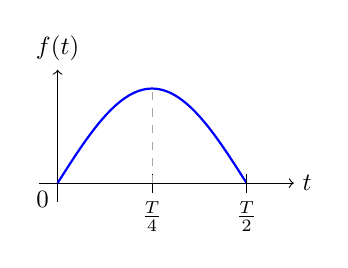
\begin{tikzpicture}[scale=1.2, every node/.style={scale=0.9}] % Fig 2
										\newcommand{\TimePeriodExTenVTwo}{4.0}
										\newcommand{\omegaZeroDegExTenVTwo}{360/\TimePeriodExTenVTwo}
										\draw[->] (-0.2,0) -- (\TimePeriodExTenVTwo/2+0.5,0) node[right] {$t$}; % Axis only up to T/2
										\draw[->] (0,-0.2) -- (0,1.2) node[above] {$f(t)$};
										\node[below left] at (0,0) {$0$};
										\draw[thick, blue, domain=0:{\TimePeriodExTenVTwo/2}, samples=100] plot (\x, {sin(\omegaZeroDegExTenVTwo*\x)});
										\draw (\TimePeriodExTenVTwo/4,0.1) -- (\TimePeriodExTenVTwo/4,-0.1) node[below] {$\frac{T}{4}$};
										\draw (\TimePeriodExTenVTwo/2,0.1) -- (\TimePeriodExTenVTwo/2,-0.1) node[below] {$\frac{T}{2}$};
										\draw[dashed, gray!70] (\TimePeriodExTenVTwo/4,0) -- (\TimePeriodExTenVTwo/4,1);
									\end{tikzpicture}
									\caption{单个正弦半波的图像 }
									\label{fig:L15_single_half_sine_fig2}
								\end{figure}
								\noindent\textbf{解 (Solution for Example 10):} \\
								\[sin\frac{2\pi}{T}t + \sin\frac{2\pi}{T}\left(t - \frac{T}{2}\right) = \sin\frac{2\pi}{T}t \cdot \chi_{\left(0, \frac{T}{2}\right)} \]
								
								故
								$f(t) = \sin\left(\frac{2\pi}{T}t\right)u(t) + \sin\left(\frac{2\pi}{T}\left(t-\frac{T}{2}\right)\right)u\left(t-\frac{T}{2}\right)$.
								(等价于 $f(t) = \sin\left(\frac{2\pi}{T}t\right)$ for $t \in [0, T/2]$ and $0$ otherwise。)
								
								\[  \mathcal{L}\left(\sin(\frac{2\pi}{T} t) \cdot u(t)\right)(s) = \mathcal{L}\left(\sin\frac{2\pi}{T} t\right)(s) = \frac{\frac{2\pi}{T}}{s^2 + \left(\frac{2\pi}{T}\right)^2} \]
								
								
								
								\[ \text{利用延时性质知} \mathcal{L}\left(\sin\frac{2\pi}{T}\left(t - \frac{T}{2}\right) u\left(t - \frac{T}{2}\right)\right)(s) = e^{-\frac{T}{2}s} \cdot \frac{\frac{2\pi}{T}}{s^2 + \left(\frac{2\pi}{T}\right)^2} \]
								
								\[ \text{故} \mathcal{L}f(s) = \left(1 + e^{-\frac{T}{2}s}\right) \frac{\frac{2\pi}{T}}{s^2 + \left(\frac{2\pi}{T}\right)^2} \]
								
								
								
								\vspace{\baselineskip}
								
								% --- Example 11: Periodic Half-wave Rectified Sine ---
								\begin{example}
									$f_T$ 为 T 周期函数。\\
									\begin{figure}[h]
										\centering
										\includegraphics[width=0.7\linewidth]{"picture/lecture 15 周期半正弦波"}
										\caption{}
										\label{fig:lecture-15-周期半正弦波}
									\end{figure}
									其中 $f_T x_{(0, \frac{T}{2})}$ 为例10中的半波正弦,$\sin \frac{2\pi}{T} t x_{(0, \frac{T}{2})}$。求 $\mathcal{L} f_T(s)$。
									
									
									
									
									\textbf{解:}
									
									由上一个例题可知
									\[
									\mathcal{L}\left(\sin\frac{2\pi}{T}t \cdot x_{(0, \frac{T}{2})}\right)(s) = \frac{\frac{2\pi}{T}}{s^2 + \left(\frac{2\pi}{T}\right)^2} \cdot \left(1 + e^{-\frac{T}{2} s}\right)
									\]
									
									利用周期性:
									\[
									\mathcal{L} f_T(s) = \frac{1}{1 - e^{-T s}} \cdot \mathcal{L}\left(\sin\frac{2\pi}{T} t \cdot x_{(0, \frac{T}{2})}\right)(s)
									\]
									\[
									= \frac{1}{1 - e^{-T s}} \cdot \frac{\frac{2\pi}{T}}{s^2 + \left(\frac{2\pi}{T}\right)^2} \cdot \left(1 + e^{-\frac{T}{2} s}\right)
									\]
									
									注:当 $\tilde{f}_T$ 为 $\frac{T}{2}$ 周期时,
									\[
									\mathcal{L} \tilde{f}_T(s) = \frac{1}{1 - e^{-\frac{T}{2} s}} \cdot \left[ \frac{\frac{2\pi}{T}}{s^2 + \left(\frac{2\pi}{T}\right)^2} \cdot \left(1 + e^{-\frac{T}{2} s}\right) \right]
									\]
									
									
									\begin{figure}[h]
										\centering
										\includegraphics[width=0.7\linewidth]{"picture/lecture 15 半波整流正弦波"}
										\caption{}
										\label{fig:lecture-15-半波整流正弦波}
									\end{figure}
									
									
									
								\end{example}
								
							} % End of section content brace
							
							
						} % End of chapter content brace
						
						
						\part{Lecture 16 Laplace 变换的逆变换}
						
						{\chapter{Laplace 变换的逆变换公式与计算}
							{ % Start of chapter content brace
								
								\section{逆变换公式的找寻 }
								{ % Start of section content brace
									记
									\[
									F(z) = \mathcal{L}\{f(t)\} = \int_{0}^{\infty} f(t) \mathrm{e}^{-zt} \,\mathrm{d}t, \quad z = \beta + i\omega, \ Re(z) > 0
									\]
									
									\begin{equation}
										F(z) = \int_{-\infty}^{\infty} \left[ f(t) \mathrm{e}^{-\beta t} \chi_{(0,+\infty)}(t) \right] \mathrm{e}^{-i\omega t} \,\mathrm{d}t
									\end{equation}
									
									即
									\begin{equation}
										\mathcal{F}\left\{ f(t) \mathrm{e}^{-\beta t} \chi_{(0,+\infty)}(t) \right\} (\omega) = \frac{1}{\sqrt{2\pi}} F(\beta + i\omega).
									\end{equation}
									
									由逆公式知
									\[
									f(t) \mathrm{e}^{-\beta t} \chi_{(0,+\infty)}(t) = \frac{1}{2\pi} \int_{-\infty}^{\infty} F(\beta + i\omega) \mathrm{e}^{+i\omega t} \,\mathrm{d}\omega
									\]
									
									故
									\[
									f(t) \chi_{(0,+\infty)}(t) = \frac{1}{2\pi} \int_{-\infty}^{\infty} F(\beta + i\omega) \mathrm{e}^{\beta t} \mathrm{e}^{+i\omega t} \,\mathrm{d}\omega
									\]
									
									\begin{equation}
										= \frac{1}{2\pi} \int_{-\infty}^{\infty} F(\beta + i\omega) \mathrm{e}^{(\beta + i\omega) t} \,\mathrm{d}\omega
									\end{equation}
									
									
									
									
									
									令 $z = \beta+i\omega$. 则 $\diff z = i \diff \omega$, 即 $\diff \omega = \frac{\diff z}{i}$.
									当 $\omega \to -\infty$, $z \to \beta-i\infty$.
									当 $\omega \to +\infty$, $z \to \beta+i\infty$.
									积分路径是在复平面上从 $\beta-i\infty$ 到 $\beta+i\infty$ 的一条垂直直线。
									代入可得 (称为 Bromwich 积分):
									\begin{equation}
										\begin{aligned}
											f(t) &= \frac{1}{2\pi} \int_{\beta-i\infty}^{\beta+i\infty} F(z) e^{zt} \frac{\diff z}{i} \\
											&= \frac{1}{2\pi i} \int_{\beta-i\infty}^{\beta+i\infty} F(z) e^{zt} \diff z \quad (t>0)
										\end{aligned}
									\end{equation}
									这条积分路径通常记为 $Br$. $\beta$ 必须大于 $F(z)$ 所有奇点的实部。
									
									\begin{figure}[h]
										\centering
										\includegraphics[width=0.4\linewidth]{"picture/lecture 16 1.1"}
										\caption{}
										\label{fig:lecture-16-1.1}
									\end{figure}
									
									
									
								} % End of section content brace
								
								
								
								
								
								
								\section{利用留数定理计算逆变换}
								{ % Start of section content brace
									\begin{theorem}[逆 Laplace 变换的留数计算法] \label{thm:L16_inverse_laplace_residue_revised}
										设 $F(z) = \mathcal{L}\{f(t)\}(z)$。如果 $F(z)$ 满足以下条件:
										\begin{enumerate}
											\item $F(z)$ 在复平面内除了有限个孤立奇点 $z_1, z_2, \dots, z_n$ 外处处解析。
											\item 所有奇点 $z_k$ 均位于某垂直直线 $\text{Re}(z) = \beta_0$ 的左侧 (即 $\text{Re}(z_k) < \beta_0$ for all $k$)。
											\item $\lim_{|z|\to\infty} F(z) = 0$ (当 $z$ 在适当的左半圆弧上,例如 $\text{Re}(z) \le \beta_0$ 的区域内)。
										\end{enumerate}
										则对于 $t>0$, 逆 Laplace 变换可以通过以下公式计算:
										\[ f(t) = \frac{1}{2\pi i} \int_{\beta-i\infty}^{\beta+i\infty} F(z)e^{zt} \diff z = \sum_{k=1}^{n} \text{Res}\left[F(z)e^{zt},z_k\right] \]
										其中积分路径 $\text{Re}(z)=\beta$ 是一条位于所有奇点 $z_k$ 右侧的垂直直线 (即 $\beta > \beta_0$)。
									\end{theorem}
									
									\textbf{证明思路 (Proof Idea):}
									\begin{enumerate}[label=\arabic*)] % Numbered list as in your notes
										\item \textbf{构造闭合围线 (Constructing a closed contour $C = L_R + C_R$):}
										\begin{figure}[h]
											\centering
											\includegraphics[width=0.4\linewidth]{"picture/lecture 16 2.1"}
											\caption{}
											\label{fig:lecture-16-2 .1}
										\end{figure}
										
										\begin{itemize}
											\item $L_R$: 从 $\beta-iR$ 到 $\beta+iR$ 的直线段 (Bromwich 路径的一部分)。
											\item $C_R$: 一个位于直线 $L_R$ 左侧的半圆弧,使得所有 $F(z)$ 的奇点 $z_1, \dots, z_n$ 都被包含在由 $L_R$ 和 $C_R$ 组成的闭合围线 $C$ 内部。
											
										\end{itemize}
										% (LaTeX TikZ figure for the first contour sketch would go here if requested)
										% You requested no figures for this part.
										
										\item \textbf{选择足够大的 $R$ (Choosing $R$ large enough):}
										选择 $R$ 足够大,使得所有奇点 $z_1, \dots, z_n$ 都位于闭合围线 $C = L_R + C_R$ 的内部区域。
										根据柯西留数定理 (Cauchy's Residue Theorem):
										\begin{equation}
											\oint_C F(z)e^{zt} \diff z = 2\pi i \sum_{k=1}^{n} \text{Res}\left[F(z)e^{zt},z_k\right] 
										\end{equation}
										即
										\begin{equation}
											\int_{\beta-iR}^{\beta+iR} F(z)e^{zt} \diff z + \int_{C_R} F(z)e^{zt} \diff z = 2\pi i \sum_{k=1}^{n} \text{Res}\left[F(z)e^{zt},z_k\right] 
										\end{equation}
										
										\item \textbf{Jordan 引理的应用 (Application of Jordan's Lemma):}
										
										我们需要证明当 $R \to \infty$ 时,$\int_{C_R} F(z)e^{zt} \diff z \to 0$.
										Jordan 引理的条件通常是:
										\begin{itemize}
											\item[i)] $F(z)$ 在 $\text{Re}(z) \le \beta$ (除去有限个奇点外) 解析。
											\item[ii)] 当 $z$ 位于 $C_R$ 上(即 $|z-\alpha|=R'$ 或类似定义,且 $\text{Re}(z) \le \beta$) 并且 $R' \to \infty$ 时,$F(z) \to 0$。
										\end{itemize}
										则对于 $t>0$,
										\[ \lim_{R\to\infty} \int_{C_R} F(z)e^{zt} \diff z = 0 \]
										
										
										\item \textbf{得到逆变换公式 (Obtaining the inverse transform formula):}
										当 $R \to \infty$ 时,由于 $\int_{C_R} F(z)e^{zt} \diff z \to 0$ (对于 $t>0$),我们得到:
										\[ \int_{\beta-i\infty}^{\beta+i\infty} F(z)e^{zt} \diff z = 2\pi i \sum_{k=1}^{n} \text{Res}\left[F(z)e^{zt},z_k \right] \]
										所以,对于 $t>0$:
										\begin{equation}
											f(t) = \frac{1}{2\pi i} \int_{\beta-i\infty}^{\beta+i\infty} F(z)e^{zt} \diff z = \sum_{k=1}^{n} \text{Res}\left[F(z)e^{zt},z_k \right] 
										\end{equation}
									\end{enumerate}
									\textbf{求逆 $\implies$ 转为求留数计算!
									} % End of section content brace
									
									
									
									\section{孤立奇点与留数计算基础 }
									{ % Start of section content brace
										\subsection{孤立奇点 (Isolated Singularities)}
										{ % Start of subsection content brace
											设 $a \in \C$ 是函数 $f(z)$ 的一个孤立奇点,指的是存在 $\delta > 0$,使得 $f(z)$ 在去心邻域 $U'(a, \delta) = \{z \in \C : 0 < |z-a| < \delta\}$ 内解析,但在点 $a$ 本身无定义或不可导。
											
											\textbf{分类 (Classification):}
											\begin{enumerate}[label=\arabic*)]
												\item \textbf{可去奇点 (Removable Singularity):}
												如果 $\lim_{z\to a} f(z) = A$ 存在且为有限值 ($A \neq \infty$)。
												(可以通过补充定义 $f(a)=A$ 使函数在 $a$ 点解析。)
												\item \textbf{极点 (Pole):}
												如果 $\lim_{z\to a} f(z) = \infty$.
												(此时 $f(z)$ 可以在 $a$ 的邻域表示为 $f(z) = \frac{g(z)}{(z-a)^m}$, 其中 $g(a) \neq 0$ 且有限, $m \in \N^+$ 为极点的阶。)
												\item \textbf{本性奇点 (Essential Singularity):}
												如果 $\lim_{z\to a} f(z)$ 不存在 (既不趋于有限值也不趋于 $\infty$)。
												(例如 $f(z) = e^{1/z}$ 在 $z=0$ 处。)
											\end{enumerate}
										} % End of subsection content brace
									} % End of section content brace
									
									\subsection{Laurent 定理 }
									{ % Start of section content brace
										\begin{theorem}[Laurent 定理] \label{thm:L16_laurent_series}
											设函数 $f(z)$ 在圆环域 $D = \{z \in \C : r < |z-a| < R\}$ 内解析 。
											则对于 $D$ 内的任意一点 $z$, $f(z)$ 可以唯一地表示为 Laurent 级数:
											\begin{equation}
												f(z) = \sum_{k=-\infty}^{\infty} c_k (z-a)^k = \sum_{k=0}^{\infty} c_k (z-a)^k + \sum_{k=1}^{\infty} c_{-k} (z-a)^{-k} 
											\end{equation}
											其中系数 $c_k$ 由下式给出:
											\begin{equation}
												c_k = \frac{1}{2\pi i} \oint_C \frac{f(\zeta)}{(\zeta-a)^{k+1}} \diff \zeta, \quad k = 0, \pm 1, \pm 2, \dots 
											\end{equation}
											积分围道 $C$ 是圆环域 $D$ 内任何一条环绕点 $a$ 的简单闭合正向曲线 (例如 $|z-a|=\rho$, 其中 $r < \rho < R$)。
											级数的展开式是唯一的。
										\end{theorem}
										
										\textbf{证明思路 (Proof Idea for Laurent's Theorem):}
										
										\begin{figure}[h]
											\centering
											\includegraphics[width=0.4\linewidth]{"picture/lecture 16 3.1"}
											\caption{}
											\label{fig:lecture-16-3.1}
										\end{figure}
										
										\begin{enumerate}[label=\arabic*)]
											\item 对于圆环域 $D: r < |z-a| < R$ 内的任意一点 $z$,取两个同心圆 $C_1: |\zeta-a|=R_1$ 和 $C_2: |\zeta-a|=r_1$ (逆时针为 $C_1$, 顺时针为 $C_2$ (或 $C_1$ 和 $-C_2$ 都逆时针)),使得 $r < r_1 < |z-a| < R_1 < R$。
											函数 $f(\zeta)$ 在由 $C_1$ 和 $C_2$ 界定的闭圆环域(除去 $z$ 点的一个小邻域)内解析。
											根据柯西积分公式的推广(或柯西-古尔萨定理应用于多连通域):
											对于圆环域 $r_1 < |\zeta-a| < R_1$ 内的 $z$,
											\begin{equation}
												f(z) = \frac{1}{2\pi i} \oint_{C_1} \frac{f(\zeta)}{\zeta-z} \diff \zeta - \frac{1}{2\pi i} \oint_{C_2} \frac{f(\zeta)}{\zeta-z} \diff \zeta 
											\end{equation}
											(注意 $C_1$ 和 $C_2$ 均取逆时针方向,所以 $C_2$ 项前有负号。)
											
											\item \textbf{处理第一个积分 (对应级数的解析部分/正幂项):}
											对于 $\zeta \in C_1$ (即 $|\zeta-a|=R_1$), 我们有 $|z-a| < R_1 = |\zeta-a|$.
											所以 $\left|\frac{z-a}{\zeta-a}\right| < 1$.
											\[ \frac{1}{\zeta-z} = \frac{1}{(\zeta-a) - (z-a)} = \frac{1}{\zeta-a} \cdot \frac{1}{1 - \frac{z-a}{\zeta-a}} \]
											利用几何级数展开 $\frac{1}{1-q} = \sum_{k=0}^\infty q^k$ (当 $|q|<1$):
											\[ \frac{1}{\zeta-z} = \frac{1}{\zeta-a} \sum_{k=0}^{\infty} \left(\frac{z-a}{\zeta-a}\right)^k = \sum_{k=0}^{\infty} \frac{(z-a)^k}{(\zeta-a)^{k+1}} \]
											这个级数在 $C_1$ 上一致收敛。逐项积分得到:
											\begin{align*}
												\frac{1}{2\pi i} \oint_{C_1} \frac{f(\zeta)}{\zeta-z} \diff \zeta &= \frac{1}{2\pi i} \oint_{C_1} f(\zeta) \left( \sum_{k=0}^{\infty} \frac{(z-a)^k}{(\zeta-a)^{k+1}} \right) \diff \zeta \\
												&= \sum_{k=0}^{\infty} \left( \frac{1}{2\pi i} \oint_{C_1} \frac{f(\zeta)}{(\zeta-a)^{k+1}} \diff \zeta \right) (z-a)^k \\
												&= \sum_{k=0}^{\infty} c_k (z-a)^k
											\end{align*}
											其中 $c_k = \frac{1}{2\pi i} \oint_{C_1} \frac{f(\zeta)}{(\zeta-a)^{k+1}} \diff \zeta$ for $k \ge 0$.
											
											\textbf {注:}可逐项积分是由于级数$\sum_{k=0}^{\infty} \frac{(z-a)^k}{(\zeta-a)^{k+1}}$在 $C_1$ 上关于参数$z$一致收敛.
											
											又 \(f(\zeta)\) 在 $C_1$ 上有界,则$\sum_{k=0}^{\infty} \frac{f(\zeta)(z-a)^k}{(\zeta-a)^{k+1}}$在 $C_1$ 上一致收敛.
											
											
											\item \textbf{处理第二个积分 (对应级数的主要部分/负幂项) :}
											% (您的笔记的当前图片从此步骤开始)
											对于 $\zeta \in C_2$ (即 $|\zeta-a|=r_1$), 我们有 $|\zeta-a| = r_1 < |z-a|$.
											所以 $\left|\frac{\zeta-a}{z-a}\right| < 1$.
											回顾:
											\[ -\frac{1}{2\pi i} \oint_{C_2} \frac{f(\zeta)}{\zeta-z} \diff \zeta = \frac{1}{2\pi i} \oint_{C_2} \frac{f(\zeta)}{z-\zeta} \diff \zeta \]
											我们展开 $\frac{1}{z-\zeta}$:
											\begin{align*}
												\frac{1}{z-\zeta} &= \frac{1}{(z-a) - (\zeta-a)} \\
												&= \frac{1}{z-a} \cdot \frac{1}{1 - \frac{\zeta-a}{z-a}} \\
												&= \frac{1}{z-a} \sum_{j=0}^{\infty} \left(\frac{\zeta-a}{z-a}\right)^j \quad \text{(因为 } \left|\frac{\zeta-a}{z-a}\right|<1 \text{)} \\
												&= \sum_{j=0}^{\infty} \frac{(\zeta-a)^j}{(z-a)^{j+1}}
											\end{align*}
											这个级数在 $C_2$ 上关于 $\zeta$ 一致收敛。逐项积分得到:
											\begin{align*}
												\frac{1}{2\pi i} \oint_{C_2} \frac{f(\zeta)}{z-\zeta} \diff \zeta &= \frac{1}{2\pi i} \oint_{C_2} f(\zeta) \left( \sum_{j=0}^{\infty} \frac{(\zeta-a)^j}{(z-a)^{j+1}} \right) \diff \zeta \\
												&= \sum_{j=0}^{\infty} \left( \frac{1}{2\pi i} \oint_{C_2} f(\zeta)(\zeta-a)^j \diff \zeta \right) (z-a)^{-(j+1)}
											\end{align*}
											令 $k' = j+1$. 当 $j=0, k'=1$; 当 $j \to \infty, k' \to \infty$.
											再令 $c_{-k'} = \frac{1}{2\pi i} \oint_{C_2} f(\zeta)(\zeta-a)^{k'-1} \diff \zeta$ for $k' \ge 1$.
											(这等价于 $c_k = \frac{1}{2\pi i} \oint_{C_2} \frac{f(\zeta)}{(\zeta-a)^{k+1}} \diff \zeta$ for $k = -k' \le -1$ )
											则此部分可以写为:
											\[ \sum_{k'=1}^{\infty} c_{-k'} (z-a)^{-k'} = \sum_{k=1}^{\infty} \frac{c_{-k}}{(z-a)^k} \]
											
											
											\textbf{注 (Note on uniform convergence):}
											可逐项积分是由于级数 $\sum \frac{1}{(\zeta-a)^{k+1}}(z-a)^k$ (对于第一个积分) 和 $\sum \frac{(\zeta-a)^j}{(z-a)^{j+1}}$ (对于第二个积分) 在各自的积分路径 $C_1$ 和 $C_2$ 上关于 $\zeta$ 一致收敛 (因为 $z$ 是固定的,且满足收敛半径条件),并且 $f(\zeta)$ 有界。
											
											\item \textbf{综合步骤 1, 2, 3 (Combining steps 1, 2, and 3):}
											\begin{equation}
												f(z) = \sum_{k=0}^{\infty} c_k (z-a)^k + \sum_{k=1}^{\infty} c_{-k} (z-a)^{-k}  = \sum_{k=-\infty}^{\infty} c_k (z-a)^k
											\end{equation}
											其中系数 $c_k$ (如前所述,由于被积函数在圆环内解析) 可以用统一的积分路径 $C$ ($r < |\zeta-a|=\rho < R$) 表示:
											\begin{equation}
												c_k = \frac{1}{2\pi i} \oint_C \frac{f(\zeta)}{(\zeta-a)^{k+1}} \diff \zeta, \quad \forall \rho \in (r,R), \text{ 与 } z \text{ 无关}. 	\end{equation}
											\textbf{注 :} 展开式是唯一的。
											
											
											\item \textbf{推论 (Corollary): Taylor 级数 (Taylor Series)} \\
											如果 $f(z)$ 在圆盘 $|z-a|<R$ 内解析,则 Laurent 级数中所有负幂项的系数 $c_k$ (对于 $k<0$) 均为零。
											即 $c_{-1}, c_{-2}, \dots$ 都等于零。
											
											这是因为当 $k < 0$ (例如 $k = -m$,$m \ge 1$), $c_k = c_{-m} = \frac{1}{2\pi i} \oint_C f(\zeta)(\zeta-a)^{m-1} \diff \zeta$.
											由于 $f(\zeta)(\zeta-a)^{m-1}$ 在 $C$ 内部及边界上解析 (因为 $f$ 在 $|z-a|<R$ 内解析,且 $m \ge 1$),根据柯西-古尔萨定理,这个积分为零。
											此时,Laurent 级数退化为 Taylor 级数:
											\[ f(z) = \sum_{k=0}^{\infty} c_k (z-a)^k \]
											其中 $c_k = \frac{1}{2\pi i} \oint_C \frac{f(\zeta)}{(\zeta-a)^{k+1}} \diff \zeta = \frac{f^{(k)}(a)}{k!}$ (根据柯西高阶导数公式)
											
											
											
											
										\end{enumerate}
									} 
									
									\subsection{Laurent 级数与奇点分类 }
									{ % Start of subsection content brace
										设 $a \in \C$ 是函数 $f(z)$ 的一个孤立奇点。这意味着 $\exists \delta > 0$,使得 $f(z)$ 在去心邻域 $U'(a, \delta) = \{z \in \C : 0 < |z-a| < \delta\}$ 内解析。
										在此去心邻域内,$f(z)$ 有 Laurent 级数展开:
										\[ f(z) = \sum_{k=-\infty}^{\infty} c_k (z-a)^k \]
										其中 
										\[c_k = \frac{1}{2\pi i} \oint_{C} \frac{f(\zeta)}{(\zeta-a)^{k+1}} \diff \zeta\]
										
										$C: |\zeta-a|=\rho$, $0 < \rho < \delta$.
										级数可以分为两部分:
										\begin{itemize}
											\item \textbf{解析部分 (Analytic Part) 或 Taylor 部分或正则部分:} $\sum_{k=0}^{\infty} c_k (z-a)^k$
											\item \textbf{主要部分 (Principal Part):} $\sum_{k=-\infty}^{-1} c_k (z-a)^k = \sum_{j=1}^{\infty} c_{-j} (z-a)^{-j}$
										\end{itemize}
										
										\begin{theorem}[奇点与 Laurent 级数的关系] \label{thm:L16_singularities_laurent}
											设 $a$ 是 $f(z)$ 的孤立奇点。
											\begin{enumerate}[label=\arabic*)]
												\item $a$ 是 $f(z)$ 的\textbf{可去奇点} $\iff$ $f(z) = \sum_{k=0}^{\infty} c_k (z-a)^k$ for $0 < |z-a| < \delta$.即 $f(z)$ 在 $a$ 点的 Laurent 级数的主要部分为零 (即 $c_k=0$ for all $k < 0$)。
												
												\begin{proof}\
													如果 $a$ 是可去奇点,则 $\lim_{z\to a} f(z) = A$ (有限)。这意味着 $f(z)$ 在 $a$ 的某个去心邻域 $U'(a,\delta_1)$ 内有界,即 $|f(z)| \le M$ for $z \in U'(a,\delta_1)$.
													
													对于 Laurent 级数的系数 $c_{-k}$ ($k \ge 1$):
													\[
													c_{-k} = \frac{1}{2\pi i} \oint_{|\zeta-a|=\rho} f(\zeta)(\zeta-a)^{k-1} \, \mathrm{d}\zeta \quad (0 < \rho < \delta_1)
													\]	
													
													\[
													|c_{-k}| \leq \left| \frac{1}{2\pi i} \int_{|\zeta-a|=\rho} \frac{f(\zeta)}{(\zeta-a)^{-k+1}} \,d\zeta \right|
													\]
													\[
													\leq \frac{M}{2\pi} \int_{|\zeta-a|=\rho} |\zeta-a|^{k-1} \,d\zeta
													\]
													\[
													= \frac{M}{2\pi} \rho^{k-1} \int_{|\zeta-a|=\rho} |\,d\zeta|
													\]
													\[
													= \frac{M}{2\pi} \rho^{k-1} \cdot 2\pi \rho = M \rho^k
													\]
													
													
													
													
													由于上式对任意 $0 < \rho < \delta_1$ 成立,令 $\rho \to 0^+$. 因为 $k \ge 1$, $\rho^k \to 0$.
													所以 $c_{-k}=0$ for all $k \ge 1$.因此,主要部分为零. 
													
													故$f(z) = \sum_{k=0}^{\infty} c_k (z-a)^k$.	此时 $c_0 = \lim_{z\to a} f(z) = A$.
												\end{proof}
												
												
												
												
												
												\item $a$ 是 $f(z)$ 的 $m$ \textbf{阶极点} ($m \in \N^+$) $\iff$ $f(z) = \sum_{k=-m}^{\infty} c_k (z-a)^k $.即 $f(z)$ 在 $a$ 点的 Laurent 级数的主要部分中,最低次幂为 $(z-a)^{-m}$ 且系数 $c_{-m} \neq 0$ (即 $c_k=0$ for $k < -m$, and $c_{-m} \neq 0$)。
												
												\begin{proof}\
													如果 $a$ 是 $f(z)$ 的极点,则 $a$ 不可能是 $f(z)$ 的零点的聚点。
													
													则 $a$ 为 $\frac{1}{f(z)}$ 的可去奇点,且 $\lim_{z \to a} f(z) = \infty$。
													
													$\Rightarrow$ $\lim_{z \to a} \frac{1}{f(z)} = 0$,即 $\frac{1}{f(z)} = \sum_{k=m}^{\infty} \frac{b_k}{(z-a)^k}$。
													
													设 $\phi(z)$ 在 $z=a$ 处解析,$\phi(a) = C_m \neq 0$。
													
													故$z=a$时, $f(z) = \frac{1}{(z-a)^m} \frac{1}{\phi(z)}$。
													
													$\phi(z)^{-1}$ 在 $z=a$ 处解析 $\Rightarrow \frac{1}{\phi(z)} = \sum_{k=0}^{\infty} b_k (z-a)^k$,其中 $b_0 = \frac{1}{\phi(a)} = \frac{1}{C_m}$。
													
													则 $f(z) = \frac{1}{(z-a)^m} \cdot \frac{1}{\phi(z)} = \frac{1}{(z-a)^m} \sum_{k=0}^{\infty} b_k (z-a)^k$。
													
													即
													\[
													f(z) = \frac{b_0}{(z-a)^m} + \frac{b_1}{(z-a)^{m-1}} + \dots + b_m + \sum_{k=1}^{\infty} b_{k+m} (z-a)^k.
													\]
													
													由 Laurent 级数展开式的唯一性知,$f$ 的主要部分只有有限项。
													
													反之,若 $f$ 的主要部分只有有限项,则
													\[
													f(z) = \frac{\psi(z)}{(z-a)^m} \quad (m \geq 1), \quad \psi(z) = \sum_{k=0}^{\infty} b_k (z-a)^k,
													\]
													其中 $b_0 = \psi(a) \neq 0$。
													
													则 $\lim_{z \to a} f(z) = \infty$,即 $a$ 为极点。
												\end{proof}
												
												
												
												
												
												
												
												
												
												\item $a$ 是 $f(z)$ 的\textbf{本性奇点}$f(z) = \sum_{k=-\infty}^{\infty} c_k (z-a)^k $
											\end{enumerate},即 $\iff$ $f(z)$ 在 $a$ 点的 Laurent 级数的主要部分有无穷多项非零系数。 
										\end{theorem}
										
										\begin{proof}\
											如果 $a$ 是本性奇点,则其 Laurent 级数中主要部分有无穷多项非零系数。
											这可以由排除法得到:它既不是可去奇点(主要部分不为零),也不是极点(主要部分不是有限项)。
											(根据 Picard 大定理,函数在本性奇点的任意小邻域内取到除至多一个值外的所有复数值。)
										\end{proof}
										
										
										
									} % End of subsection content brace
								}
								
								\subsection{留数的定义与计算 }
								{ % Start of section content brace
									
									\begin{definition}[留数 (Residue)] \label{def:L16_residue}
										设函数 $f(z)$ 在点 $a$ 的去心邻域 $U'(a,\delta) = \{z \in \C : 0 < |z-a| < \delta\}$ 内解析。
										称积分值
										\[ \frac{1}{2\pi i} \oint_{|\zeta-a|=\rho} f(\zeta) \diff \zeta \]
										为函数 $f(z)$ 在孤立奇点 $a$ 处的\textbf{留数} (Residue),其中 $\rho$ 是任何满足 $0 < \rho < \delta$ 的实数。
										记作 $\text{Res}[f(z), a]$ 或 $\text{Res}_{z=a} f(z)$.
									\end{definition}
									
									\textbf{注 :}
									\begin{itemize}
										\item 由柯西积分定理 (Cauchy's Integral Theorem),留数 $\text{Res}_{z=a} f(z)$ 的值与积分半径 $\rho$ 的选取无关 (只要 $0 < \rho < \delta$,且路径不跨过其他奇点)。
										\item 如果 $f(z)$ 在点 $a$ 处解析 (即 $a$ 不是奇点,或者是可去奇点且已补充定义),则根据柯西-古尔萨定理 (Cauchy-Goursat Theorem),$\oint_{|\zeta-a|=\rho} f(\zeta) \diff \zeta = 0$,因此 $\text{Res}_{z=a} f(z) = 0$.
									\end{itemize}
									
									\begin{theorem}[留数与 Laurent 级数系数的关系] \label{thm:L16_residue_laurent_coeff}
										设 $a$ 是 $f(z)$ 的孤立奇点。则 $f(z)$ 在点 $a$ 的留数等于其在该点 Laurent 级数展开式中 $(z-a)^{-1}$ 项的系数 $c_{-1}$。
										即
										\begin{equation}
											\text{Res}_{z=a} f(z) = c_{-1} = \frac{1}{2\pi i} \oint_{C} f(\zeta) \diff \zeta 
										\end{equation}
										(其中 $C: |\zeta-a|=\rho$, $0 < \rho < \delta$)
									\end{theorem}
									\begin{proof}\
										$f(z)$ 在 $a$ 的去心邻域内的 Laurent 级数展开为
										\[
										f(z) = \sum_{k=-\infty}^{\infty} c_k (z-a)^k.
										\]
										系数
										\[
										c_k = \frac{1}{2\pi i} \oint_C \frac{f(\zeta)}{(\zeta-a)^{k+1}} \, \mathrm{d}\zeta.
										\]
										当 $k = -1$ 时,这正是 $\text{Res}_{z=a} f(z)$ 的定义
										\[
										c_{-1} = \frac{1}{2\pi i} \oint_C \frac{f(\zeta)}{(\zeta-a)^{-1+1}} \, \mathrm{d}\zeta = \frac{1}{2\pi i} \oint_C f(\zeta) \, \mathrm{d}\zeta.
										\]
										
										
										从 $f$ 的 Laurent 级数也可计算得知:
										\begin{align*}
											\text{Res}_{z=a} f(z) &= \frac{1}{2\pi i} \int_{|z-a|=\rho} f(z) \, dz \\
											&= \frac{1}{2\pi i} \int_{|z-a|=\rho} \sum_{k=-\infty}^{\infty} c_k (z-a)^k \, dz \\
											&= \frac{1}{2\pi i} \int_{|z-a|=\rho} \sum_{k=0}^{\infty} c_k (z-a)^k \, dz + \frac{1}{2\pi i} \int_{|z-a|=\rho} \sum_{k=-\infty}^{-1} c_k (z-a)^k \, dz \\
											&\quad + \frac{1}{2\pi i} \int_{|z-a|=\rho} c_{-1} \cdot \frac{1}{z-a} \, dz \\
											&= c_{-1}.
										\end{align*}
										
										
										第一个积分利用解析性($(z-a)^k$ 解析)。
										
										第二个积分利用 $\frac{1}{2\pi i} \int_{|z-a|=\rho} \frac{1}{(z-a)^k} \, dz = \frac{d^{k-1}}{dx^{k-1}} (1) = 0$.
										
										第三个积分利用 $\int_{|z-a|=\rho} \frac{1}{z-a} \, dz = 2\pi i$.
									\end{proof}
									
									
									
									
									
									
									\vspace{\baselineskip}
									
									\textbf{孤立奇点的留数计算:}
									\begin{enumerate}[label=(\roman*)]
										\item \textbf{如果 $a$ 是可去奇点:}
										由 Laurent 级数特征,$c_{-1}=0$. 所以 $\text{Res}_{z=a} f(z) = 0$.
										
										\item \textbf{如果 $a$ 是 $m$ 阶极点 ($m \ge 1$):}
										$f(z)$ 的 Laurent 级数为
										\[
										f(z) = \frac{c_{-m}}{(z-a)^m} + \dots + \frac{c_{-1}}{z-a} + c_0 + c_1(z-a) + \dots,
										\]
										其中 $c_{-m} \neq 0$。
										
										我们要求的是 $c_{-1}$。
										
										考虑函数 $\phi(z) = (z-a)^m f(z)$。则 $\phi(z)$ 在 $a$ 点解析,其 Taylor 展开为:
										\[
										\phi(z) = (z-a)^m f(z) = c_{-m} + c_{-m+1}(z-a) + \dots + c_{-1}(z-a)^{m-1} + c_0(z-a)^m + \dots
										\]
										
										$c_{-1}$ 是 $\phi(z)$ 在 $a$ 点 Taylor 展开式中 $(z-a)^{m-1}$ 项的系数。
										
										根据 Taylor 级数系数公式,
										\[
										c_{-1} = \frac{\phi^{(m-1)}(a)}{(m-1)!}.
										\]
										
										因此,
										\[
										\text{Res}_{z=a} f(z) = c_{-1} = \frac{1}{(m-1)!} \lim_{z \to a} \frac{\mathrm{d}^{m-1}}{\mathrm{d}z^{m-1}} \left[ (z-a)^m f(z) \right].
										\]
										特别地,当 $m=1$ (单极点) 时:
										\[ \text{Res}_{z=a} f(z) = c_{-1} = \lim_{z\to a} [(z-a)f(z)] \]
										
										
										\textbf{应用 (Application):} 如果 $f(z) = \frac{g(z)}{h(z)}$, 其中 $g(a)\neq 0$, $h(a)=0$ 且 $h'(a)\neq 0$ (即 $a$ 是 $h(z)$ 的一阶零点,从而 $a$ 是 $f(z)$ 的一阶极点)。
										则
										\begin{align*}
											\text{Res}_{z=a} f(z) &= \lim_{z\to a} (z-a) \frac{g(z)}{h(z)} \\
											&= \lim_{z\to a} g(z) \cdot \lim_{z\to a} \frac{z-a}{h(z)-h(a)} \quad (\text{因为 } h(a)=0) \\
											&= g(a) \cdot \frac{1}{h'(a)} = \frac{g(a)}{h'(a)}
										\end{align*}
										
										
										\item \textbf{如果 $a$ 是本性奇点:}
										留数计算通常依赖于直接求出 Laurent 级数并找出 $c_{-1}$ 项。一般没有简单的公式。
										
									\end{enumerate}
								} % End of section content brace
								
								\section{留数定理 }
								{ % Start of section content brace
									
									\begin{theorem}[留数定理 (Residue Theorem)] \label{thm:L16_residue_theorem}
										设区域 $\Omega$ 是由有限条简单闭合曲线 $\partial\Omega$ 所围成的(可能为多连通区域)。
										设函数 $f(z)$ 在 $\Omega$ 上除去有限个孤立奇点 $z_1, z_2, \dots, z_m \in \Omega$ 外处处解析,并且 $f(z)$ 在$\overline{\Omega}$上连续。
										则
										\[ \oint_{\partial\Omega} f(z) \diff z = 2\pi i \sum_{j=1}^{m} \text{Res}[f(z), z_j] \]
										其中积分沿 $\partial\Omega$ 的正向(使得区域 $\Omega$ 始终在路径的左侧)。
									\end{theorem}
									
									\textbf{证明 (Proof):} (由柯西多连通域积分定理直接推论) \\
									对每一个奇点 $z_j \in \Omega$, 构造一个小圆周 $C_j: |\zeta-z_j|=\delta_j$, 其中 $\delta_j > 0$ 足够小,使得:
									\begin{enumerate}
										\item 每个闭圆盘 $\overline{U}(z_j, \delta_j) = \{\zeta \in \C : |\zeta-z_j| \le \delta_j\}$ 都包含在 $\Omega$ 内部,即 $\overline{U}(z_j, \delta_j) \subset \Omega$.
										\item 这些小圆盘互不相交,即 $\overline{U}(z_j, \delta_j) \cap \overline{U}(z_k, \delta_k) = \emptyset$ 对于 $j \neq k$.
									\end{enumerate}
									考虑区域 $\Omega' = \Omega \setminus \bigcup_{j=1}^{m} U(z_j, \delta_j)$ (即从 $\Omega$ 中挖去所有包含奇点的小开圆盘)。
									函数 $f(z)$ 在区域 $\Omega'$ 及其边界 $\partial\Omega' = \partial\Omega \cup (\bigcup_{j=1}^{m} (-C_j))$ 上解析 (这里 $-C_j$ 表示沿 $C_j$ 的反方向积分,即顺时针)。
									根据柯西-古尔萨定理对于多连通区域(或柯西积分定理的推广),$f(z)$ 在 $\Omega'$ 的正向边界上的积分为零:
									\[ \oint_{\partial\Omega} f(z) \diff z + \sum_{j=1}^{m} \oint_{-C_j} f(z) \diff z = 0 \]
									即
									\[ \oint_{\partial\Omega} f(z) \diff z - \sum_{j=1}^{m} \oint_{C_j} f(z) \diff z = 0 \]
									(因为 $\oint_{-C_j} = -\oint_{C_j}$, 且 $C_j$ 都是逆时针正向。)
									移项可得:
									\[ \oint_{\partial\Omega} f(z) \diff z = \sum_{j=1}^{m} \oint_{C_j} f(z) \diff z \]
									根据留数的定义,$\oint_{C_j} f(z) \diff z = 2\pi i \text{Res}[f(z), z_j]$.
									所以,
									\[ \oint_{\partial\Omega} f(z) \diff z = \sum_{j=1}^{m} 2\pi i \text{Res}[f(z), z_j] = 2\pi i \sum_{j=1}^{m} \text{Res}[f(z), z_j] \]
									证毕。
									\vspace{\baselineskip}
									
									\textbf{附:一般的柯西定理 (Appendix: General Cauchy's Theorem / Cauchy-Goursat Theorem for Multiply Connected Domains)}
									\begin{theorem}[柯西-古尔萨定理 (多连通域)] \label{thm:L16_cauchy_goursat_multiply}
										若区域 $\Omega$ 是由有限条简单封闭曲线 $\partial\Omega$ 所围成的区域,$f(z)$ 在 $\Omega$ 上解析且在 $\overline{\Omega}$ 上连续,则积分 $\oint_{\partial\Omega} f(z) \, dz = 0$。
									\end{theorem}
									
									\begin{figure}[h]
										\centering
										\includegraphics[width=0.4\linewidth]{"picture/lecture 16 4.1"}
										\caption{}
										\label{fig:lecture-16-4.1}
									\end{figure}
									
									
									
								} % End of section content brace
								
								\section{示例:用留数求 Laplace 变换的逆变换 }
								{ % Start of section content brace
									(根据留数定理,若 $F(z)$ 满足一定条件,则 $f(t) = \sum_{k} \text{Res}[F(z)e^{zt}, z_k]$ for $t>0$)
									
									\begin{example}求 $F(z) = \frac{z}{z^2+1}$ 的逆变换 $f(t)$ \label{ex:L16_inv_laplace_ex1}
									\end{example}
									\noindent\textbf{解 (Solution):} \\
									令 $H(z) = F(z)e^{zt} = \frac{z e^{zt}}{z^2+1}$.
									奇点由 $z^2+1=0 \Rightarrow z^2=-1 \Rightarrow z = \pm i$.
									这两个奇点都是 $H(z)$ (也是 $F(z)$) 的一阶极点。
									
									(i) 计算在 $z=i$ 处的留数:
									\begin{align*}
										\text{Res}[H(z), i] &= \lim_{z\to i} (z-i) \frac{z e^{zt}}{(z-i)(z+i)} \\[6pt]
										&= \lim_{z\to i} \frac{z e^{zt}}{z+i} \\[6pt]
										&= \frac{i e^{it}}{i+i} = \frac{i e^{it}}{2i} = \frac{1}{2}e^{it}
									\end{align*}
									
									(ii) 计算在 $z=-i$ 处的留数:
									\begin{align*}
										\text{Res}[H(z), -i] &= \lim_{z\to -i} (z-(-i)) \frac{z e^{zt}}{(z-i)(z+i)} \\[6pt]
										&= \lim_{z\to -i} (z+i) \frac{z e^{zt}}{(z-i)(z+i)} \\[6pt]
										&= \lim_{z\to -i} \frac{z e^{zt}}{z-i} \\[6pt]
										&= \frac{-i e^{-it}}{-i-i} = \frac{-i e^{-it}}{-2i} = \frac{1}{2}e^{-it}
									\end{align*}
									故,对于 $t>0$:
									\begin{align*}
										f(t) &= \text{Res}[H(z), i] + \text{Res}[H(z), -i] \\[6pt]
										&= \frac{1}{2}e^{it} + \frac{1}{2}e^{-it} \\[6pt]
										&= \frac{e^{it} + e^{-it}}{2} = \cos(t)
									\end{align*}
									所以 $f(t) = \cos(t) u(t)$.
									\vspace{\baselineskip}
									
									\begin{example}求 $F(z) = \frac{1}{z(z-1)^2}$ 的逆变换 $f(t)$ \label{ex:L16_inv_laplace_ex2}
									\end{example}
									\noindent\textbf{解 (Solution):} \\
									令 $H(z) = F(z)e^{zt} = \frac{e^{zt}}{z(z-1)^2}$.
									奇点为 $z=0$ (一阶极点) 和 $z=1$ (二阶极点)。
									
									(i) 计算在 $z=0$ 处的留数 (一阶极点):
									\begin{align*}
										\text{Res}[H(z), 0] &= \lim_{z\to 0} (z-0) \frac{e^{zt}}{z(z-1)^2} \\[6pt]
										&= \lim_{z\to 0} \frac{e^{zt}}{(z-1)^2} \\[6pt]
										&= \frac{e^0}{(-1)^2} = \frac{1}{1} = 1
									\end{align*}
									
									(ii) 计算在 $z=1$ 处的留数 (二阶极点, $m=2$):
									\begin{align*}
										\text{Res}[H(z), 1] &= \frac{1}{(2-1)!} \lim_{z\to 1} \frac{\diff^{2-1}}{\diff z^{2-1}} \left[ (z-1)^2 \frac{e^{zt}}{z(z-1)^2} \right] \\[6pt]
										&= \lim_{z\to 1} \frac{\diff}{\diff z} \left[ \frac{e^{zt}}{z} \right] \\
										&= \lim_{z\to 1} \frac{z(te^{zt}) - e^{zt}(1)}{z^2} \\[6pt]
										&= \frac{1(te^{t}) - e^{t}(1)}{1^2} = te^t - e^t
									\end{align*}
									故,对于 $t>0$:
									\begin{align*}
										f(t) &= \text{Res}[H(z), 0] + \text{Res}[H(z), 1] \\[6pt]
										&= 1 + (te^t - e^t) = 1 + te^t - e^t
									\end{align*}
									所以 $f(t) = (1 + te^t - e^t)u(t)$.
									\vspace{\baselineskip}
									
									\begin{example}求 $F(z) = \frac{1}{(z+1)(z-2)(z+3)}$ 的逆变换 $f(t)$ \label{ex:L16_inv_laplace_ex3}
									\end{example}
									\noindent\textbf{解 (Solution):} \\
									令 $H(z) = F(z)e^{zt} = \frac{e^{zt}}{(z+1)(z-2)(z+3)}$.
									奇点为 $z=-1, z=2, z=-3$,均为一阶极点。
									
									(i) 计算在 $z=-1$ 处的留数:
									\begin{align*}
										\text{Res}[H(z), -1] &= \lim_{z\to -1} (z+1) \frac{e^{zt}}{(z+1)(z-2)(z+3)} \\[6pt]
										&= \lim_{z\to -1} \frac{e^{zt}}{(z-2)(z+3)} \\[6pt]
										&= \frac{e^{-t}}{(-1-2)(-1+3)} = \frac{e^{-t}}{(-3)(2)} = -\frac{1}{6}e^{-t}
									\end{align*}
									
									(ii) 计算在 $z=2$ 处的留数:
									\begin{align*}
										\text{Res}[H(z), 2] &= \lim_{z\to 2} (z-2) \frac{e^{zt}}{(z+1)(z-2)(z+3)} \\[6pt]
										&= \lim_{z\to 2} \frac{e^{zt}}{(z+1)(z+3)} \\[6pt]
										&= \frac{e^{2t}}{(2+1)(2+3)} = \frac{e^{2t}}{(3)(5)} = \frac{1}{15}e^{2t}
									\end{align*}
									
									(iii) 计算在 $z=-3$ 处的留数:
									\begin{align*}
										\text{Res}[H(z), -3] &= \lim_{z\to -3} (z+3) \frac{e^{zt}}{(z+1)(z-2)(z+3)} \\[6pt]
										&= \lim_{z\to -3} \frac{e^{zt}}{(z+1)(z-2)} \\[6pt]
										&= \frac{e^{-3t}}{(-3+1)(-3-2)} = \frac{e^{-3t}}{(-2)(-5)} = \frac{1}{10}e^{-3t}
									\end{align*}
									故,对于 $t>0$:
									\begin{align*}
										f(t) &= \text{Res}[H(z), -1] + \text{Res}[H(z), 2] + \text{Res}[H(z), -3] \\[6pt]
										&= -\frac{1}{6}e^{-t} + \frac{1}{15}e^{2t} + \frac{1}{10}e^{-3t}
									\end{align*}
									所以 $f(t) = \left(-\frac{1}{6}e^{-t} + \frac{1}{15}e^{2t} + \frac{1}{10}e^{-3t}\right)u(t)$.
									
									\vspace{\baselineskip}
									
									
									\begin{example}求 $F(z) = \frac{1}{z^2(z+1)}$ 的逆变换 $f(t)$ \label{ex:L16_inv_laplace_ex4}
									\end{example}
									\noindent\textbf{解 (Solution):} \\
									令 $H(z) = F(z)e^{zt} = \frac{e^{zt}}{z^2(z+1)}$.
									奇点为 $z=0$ (二阶极点) 和 $z=-1$ (一阶极点)。
									
									(i) 计算在 $z=0$ 处的留数 (二阶极点, $m=2$):
									\begin{align*}
										\text{Res}[H(z), 0] &= \frac{1}{(2-1)!} \lim_{z\to 0} \frac{\diff^{2-1}}{\diff z^{2-1}} \left[ z^2 \frac{e^{zt}}{z^2(z+1)} \right] \\[6pt]
										&= \lim_{z\to 0} \frac{\diff}{\diff z} \left[ \frac{e^{zt}}{z+1} \right] \\[6pt]
										&= \lim_{z\to 0} \frac{(z+1)(te^{zt}) - e^{zt}(1)}{(z+1)^2} \\[6pt]
										&= \frac{(0+1)(te^{0}) - e^{0}(1)}{(0+1)^2} = \frac{t-1}{1} = t-1
									\end{align*}
									
									(ii) 计算在 $z=-1$ 处的留数 (一阶极点):
									\begin{align*}
										\text{Res}[H(z), -1] &= \lim_{z\to -1} (z+1) \frac{e^{zt}}{z^2(z+1)} \\[6pt]
										&= \lim_{z\to -1} \frac{e^{zt}}{z^2} \\[6pt]
										&= \frac{e^{-t}}{(-1)^2} = e^{-t}
									\end{align*}
									故,对于 $t>0$:
									\begin{align*}
										f(t) &= \text{Res}[H(z), 0] + \text{Res}[H(z), -1] \\
										&= (t-1) + e^{-t}
									\end{align*}
									所以 $f(t) = (t-1+e^{-t})u(t)$.
									\vspace{\baselineskip}
									
									\begin{example}求 $F(z) = \ln\frac{z+1}{z-1}$ 的逆变换 $f(t)$ \label{ex:L16_inv_laplace_ex5}
									\end{example}
									\noindent\textbf{解 (Solution):} \\
									设 \( F(z) = \ln(z+1) - \ln(z-1) \)。
									
									在 \( z = -1 \) 和 \( z = 1 \) 处,是复杂的无穷多值分枝奇点,不宜直接用留数定理。我们考虑利用 Laplace 变换的性质。
									
									已知:
									\[
									\mathcal{L}\{tf(t)\}(z) = -\frac{\mathrm{d}F(z)}{\mathrm{d}z}.
									\]
									
									令 \( G(z) = F'(z) = \frac{\mathrm{d}}{\mathrm{d}z} \left( \ln\frac{z+1}{z-1} \right) \)。
									
									则:
									\begin{align*}
										G(z) &= \frac{\mathrm{d}}{\mathrm{d}z} \left( \ln(z+1) - \ln(z-1) \right) \\
										&= \frac{1}{z+1} - \frac{1}{z-1} \\
										&= \frac{(z-1) - (z+1)}{(z+1)(z-1)} \\
										&= \frac{-2}{z^2 - 1}.
									\end{align*}
									
									因此:
									\[
									\mathcal{L}\{tf(t)\}(z) = -G(z) = \frac{2}{z^2 - 1}.
									\]
									
									我们需要求:
									\[
									g(t) = \mathcal{L}^{-1}\{G(z)\}(t) = \mathcal{L}^{-1}\left\{\frac{-2}{z^2 - 1}\right\}(t).
									\]
									
									\begin{align*}
										\mathcal{L}^{-1}\left(-\frac{2}{z^2 - 1} e^{zt}\right)(t) &= \text{Res}\left(-\frac{2}{z^2 - 1} e^{zt}, z=1\right) + \text{Res}\left(-\frac{2}{z^2 - 1} e^{zt}, z=-1\right) \\[6pt]
										&= \lim_{z \to 1} \left(-\frac{2}{(z + 1)(z - 1)} e^{zt}\right) + \lim_{z \to -1} \left(-\frac{2}{(z + 1)(z - 1)} e^{zt}\right) \\[6pt]
										&= -e^{t} + e^{-t}
									\end{align*}
									
									由于:
									\[
									\mathcal{L}\{tf(t)\}(z) = -G(z),
									\]
									
									则:
									\[
									tf(t) = -g(t) = -(e^{-t} - e^t) = e^t - e^{-t}.
									\]
									
									所以,对于 \( t \geq 0 \):
									\[
									f(t) = \frac{e^t - e^{-t}}{t} = \frac{2 \sinh t}{t}.
									\]
									
									因此:
									\[
									f(t) = \frac{2 \sinh t}{t} \cdot u(t).
									\]
									\vspace{\baselineskip}
									
									\begin{example}求 $F(z) = \frac{z}{(z^2-1)^2}$ 的逆变换 $f(t)$ \label{ex:L16_inv_laplace_ex6}
									\end{example}
									\noindent\textbf{解 (Solution):} \\
									令 $H(z) = F(z)e^{zt} = \frac{z e^{zt}}{(z^2-1)^2} = \frac{z e^{zt}}{((z-1)(z+1))^2} = \frac{z e^{zt}}{(z-1)^2(z+1)^2}$.
									奇点为 $z=1$ (二阶极点) 和 $z=-1$ (二阶极点)。
									
									(i) 计算在 $z=1$ 处的留数 (二阶极点, $m=2$):
									\begin{align*}
										\text{Res}[H(z), 1] &= \lim_{z\to 1} \frac{\diff}{\diff z} \left[ (z-1)^2 \frac{z e^{zt}}{(z-1)^2(z+1)^2} \right] \\[6pt]
										&= \lim_{z\to 1} \frac{\diff}{\diff z} \left[ \frac{z e^{zt}}{(z+1)^2} \right] \\[6pt]
										&= \lim_{z\to 1} \frac{[(1)e^{zt} + z(te^{zt})](z+1)^2 - z e^{zt} [2(z+1)(1)]}{(z+1)^4} \\[6pt]
										&= \lim_{z\to 1} \frac{[(1+zt)e^{zt}](z+1) - 2z e^{zt}}{(z+1)^3} \\[6pt]
										&= \frac{[(1+t)e^t](1+1) - 2(1)e^t}{(1+1)^3} = \frac{2(1+t)e^t - 2e^t}{8} \\[6pt]
										&= \frac{2e^t + 2te^t - 2e^t}{8} = \frac{2te^t}{8} = \frac{1}{4}te^t
									\end{align*}
									
									(ii) 计算在 $z=-1$ 处的留数 (二阶极点, $m=2$):
									\begin{align*}
										\text{Res}[H(z), -1] &= \lim_{z\to -1} \frac{\diff}{\diff z} \left[ (z+1)^2 \frac{z e^{zt}}{(z-1)^2(z+1)^2} \right] \\[6pt]
										&= \lim_{z\to -1} \frac{\diff}{\diff z} \left[ \frac{z e^{zt}}{(z-1)^2} \right] \\[6pt]
										&= \lim_{z\to -1} \frac{[(1)e^{zt} + z(te^{zt})](z-1)^2 - z e^{zt} [2(z-1)(1)]}{(z-1)^4} \\[6pt]
										&= \lim_{z\to -1} \frac{[(1+zt)e^{zt}](z-1) - 2z e^{zt}}{(z-1)^3} \\[6pt]
										&= \frac{[(1-t)e^{-t}](-1-1) - 2(-1)e^{-t}}{(-1-1)^3} = \frac{-2(1-t)e^{-t} + 2e^{-t}}{-8} \\[6pt]
										&= \frac{-2e^{-t} + 2te^{-t} + 2e^{-t}}{-8} = \frac{2te^{-t}}{-8} = -\frac{1}{4}te^{-t}
									\end{align*}
									故,对于 $t>0$:
									\begin{align*}
										f(t) &= \text{Res}[H(z), 1] + \text{Res}[H(z), -1] \\[6pt]
										&= \frac{1}{4}te^t - \frac{1}{4}te^{-t} \\[6pt]
										&= \frac{t}{4}(e^t - e^{-t}) = \frac{t}{4} (2\sinh t) = \frac{1}{2}t\sinh t
									\end{align*}
									所以 $f(t) = \frac{1}{2}t\sinh t \cdot u(t)$.
									
									\noindent\textbf{另解 :}
									
									$\int_z^\infty \frac{s}{(s^2-1)^2} \diff s$. 令 $u=s^2-1$, $\diff u = 2s \diff s$.
									\[\int_z^\infty \frac{s}{(s^2-1)^2} \diff s= \int_{z^2-1}^\infty \frac{1}{u^2} \frac{1}{2} \diff u = \frac{1}{2} \left[ -\frac{1}{u} \right]_{z^2-1}^\infty = \frac{1}{2} \left( 0 - \left(-\frac{1}{z^2-1}\right) \right) = \frac{1}{2(z^2-1)} \]
									已知:
									\[
									\mathcal{L}\left\{\frac{f(t)}{t}\right\}(z) = \int_z^\infty F(s) \, \mathrm{d}s.
									\]
									
									若 \( F(z) = \frac{z}{(z^2 - 1)^2} \),我们可以通过积分找到其对应的拉普拉斯逆变换:
									
									\[
									\mathcal{L}^{-1}\left\{\int_z^\infty F(s) \, \mathrm{d}s\right\}(t) = \frac{f(t)}{t}.
									\]
									而
									\begin{align*}
										\mathcal{L}^{-1}\left(\frac{1}{2} \cdot \frac{1}{(z^2 - 1)}\right)(t) &= \text{Res}\left(\frac{1}{2} \cdot \frac{1}{(z+1)} e^{zt}, z=1\right) + \text{Res}\left(\frac{1}{2} \cdot \frac{1}{(z-1)} e^{zt}, z=-1\right) \\
										&= \lim_{z \to 1} \frac{1}{2} \cdot \frac{1}{(z+1)} e^{zt} + \lim_{z \to -1} \frac{1}{2} \cdot \frac{1}{(z-1)} e^{zt} \\
										&= \frac{1}{4} e^{t} - \frac{1}{4} e^{-t} \\
										&= \frac{1}{2} \sinh t, \quad t > 0.
									\end{align*}
									\textbf{注:}
									\begin{align*}
										\frac{1}{2} \cdot \frac{1}{z^2 - 1} &= \int_{0}^{+\infty} \frac{1}{2} \sinh t \cdot e^{-zt} \, \mathrm{d}t \\[6pt]
										\frac{\mathrm{d}}{\mathrm{d}z} \left( \frac{-2}{(z^2 - 1)^2} \right) &= \int_{0}^{+\infty} \frac{\mathrm{d}}{\mathrm{d}z} \left( \frac{1}{2} \sinh t \cdot e^{-zt} \right) \mathrm{d}t \\[6pt]
										\mathcal{L}\left( \frac{t}{2} \sinh t \right)(z) &= \frac{2}{(z^2 + 1)^2}.
									\end{align*}
									
									\begin{example}求 $F(z) = \frac{z^2}{(z^2+a^2)^2}$ 的逆变换 $f(t)$ ($a>0$) \label{ex:L16_inv_laplace_ex7_spaced}
									\end{example}
									\noindent\textbf{解 (Solution using residues):} \\
									令 $H(z) = F(z)e^{zt} = \frac{z^2 e^{zt}}{(z^2+a^2)^2} = \frac{z^2 e^{zt}}{(z-ia)^2(z+ia)^2}$.
									奇点为 $z=ia$ (二阶极点) 和 $z=-ia$ (二阶极点)。
									
									(i) 计算在 $z=ia$ 处的留数 (二阶极点, $m=2$):
									\begin{align*}
										R_1 = \text{Res}[H(z), ia] &= \lim_{z\to ia} \frac{\diff}{\diff z} \left[ (z-ia)^2 \frac{z^2 e^{zt}}{(z-ia)^2(z+ia)^2} \right] \\[6pt]
										&= \lim_{z\to ia} \frac{\diff}{\diff z} \left[ \frac{z^2 e^{zt}}{(z+ia)^2} \right] \\[8pt]
										&= \lim_{z\to ia} \frac{(2z e^{zt} + z^2 t e^{zt})(z+ia)^2 - z^2 e^{zt} [2(z+ia)]}{(z+ia)^4} \\[8pt]
										&= \lim_{z\to ia} \frac{(2z + z^2 t)e^{zt}(z+ia) - 2z^2 e^{zt}}{(z+ia)^3} \\[8pt]
										&= \frac{(2ia + (ia)^2 t)e^{iat}(ia+ia) - 2(ia)^2 e^{iat}}{(ia+ia)^3} \\[8pt]
										&= \frac{(2ia - a^2 t)e^{iat}(2ia) - 2(-a^2)e^{iat}}{(2ia)^3} \\[6pt]
										&= \frac{(-4a^2 - 2ia^3 t)e^{iat} + 2a^2 e^{iat}}{-8ia^3} \\[8pt]
										&= \frac{(-2a^2 - 2ia^3 t)e^{iat}}{-8ia^3} = \frac{-2a^2(1 + iat)e^{iat}}{-8ia^3} \\[8pt]
										&= \frac{(1 + iat)e^{iat}}{4ia} = \frac{1}{4ia}e^{iat} + \frac{t}{4}e^{iat}
									\end{align*}
									
									(ii) 计算在 $z=-ia$ 处的留数 (二阶极点, $m=2$):
									$R_2 = \overline{R_1} = \frac{i}{4a}e^{-iat} + \frac{t}{4}e^{-iat}$.
									(直接计算过程如下):
									\begin{align*}
										R_2 &= \lim_{z\to -ia} \frac{\diff}{\diff z} \left[ \frac{z^2 e^{zt}}{(z-ia)^2} \right] \\[6pt]
										&= \lim_{z\to -ia} \frac{(2z + z^2 t)e^{zt}(z-ia) - 2z^2 e^{zt}}{(z-ia)^3} \\[6pt]
										&= \frac{(-2ia - a^2 t)e^{-iat}(-2ia) - 2(-a^2)e^{-iat}}{(-2ia)^3} \\[6pt]
										&= \frac{(4i^2a^2 + 2ia^3 t)e^{-iat} + 2a^2 e^{-iat}}{-8i^3a^3} \\[6pt]
										&= \frac{(-2a^2 + 2ia^3 t)e^{-iat}}{8ia^3} = \frac{2a^2(-1 + iat)e^{-iat}}{8ia^3} \\[6pt]
										&= \frac{(-1 + iat)e^{-iat}}{4ia} = \frac{i}{4a}e^{-iat} + \frac{t}{4}e^{-iat}
									\end{align*}
									故,对于 $t>0$:
									\begin{align*}
										f(t) &= R_1 + R_2 \\[6pt]
										&= \left(\frac{1}{4ia}e^{iat} + \frac{t}{4}e^{iat}\right) + \left(\frac{i}{4a}e^{-iat} + \frac{t}{4}e^{-iat}\right) \\[6pt]
										&= \frac{1}{4ia}(e^{iat} - e^{-iat}) + \frac{t}{4}(e^{iat} + e^{-iat}) \\[6pt]
										&= \frac{1}{4ia}(2i\sin(at)) + \frac{t}{4}(2\cos(at)) \\[6pt]
										&= \frac{1}{2a}\sin(at) + \frac{t}{2}\cos(at)
									\end{align*}
									所以 $f(t) = \frac{1}{2a}(\sin(at) + at\cos(at))u(t)$.
									\vspace{\baselineskip}
									
									\noindent\textbf{另解 (卷积法):} \\
									$F(z) = \frac{z}{z^2+a^2} \cdot \frac{z}{z^2+a^2}$.
									令 $G(z) = \frac{z}{z^2+a^2}$, $g(t) = \cos(at)u(t)$.
									$f(t) = (g*g)(t) = (\cos(at) * \cos(at))(t)$.
									\begin{align*}
										f(t) &= \int_0^t \cos(a\tau)\cos(a(t-\tau)) \diff \tau \\[6pt]
										&= \int_0^t \frac{1}{2} [\cos(2a\tau - at) + \cos(at)] \diff \tau \\[6pt]
										&= \frac{1}{2} \left[ \frac{1}{2a}\sin(2a\tau - at) + \tau\cos(at) \right]_0^t \\[6pt]
										&= \frac{1}{2} \left[ \left(\frac{1}{2a}\sin(at) + t\cos(at)\right) - \left(\frac{1}{2a}\sin(-at) + 0\cdot\cos(at)\right) \right] \\[6pt]
										&= \frac{1}{2} \left[ \frac{1}{a}\sin(at) + t\cos(at) \right] \\[6pt]
										&= \frac{1}{2a}\sin(at) + \frac{t}{2}\cos(at)
									\end{align*}
									这与留数法结果一致。
									
									
									\begin{example}求 $F(z) = \frac{e^{-\pi z}}{z(z+a)}$ 的逆变换 $f(t)$ ($\pi>0$ constant, $a \neq 0$) \label{ex:L16_inv_laplace_ex8_corrected_spaced}
									\end{example}
									\noindent\textbf{解 (Solution):} \\
									令 $H(z) = F(z)e^{zt} = \frac{e^{-\pi z}e^{zt}}{z(z+a)} = \frac{e^{(t-\pi)z}}{z(z+a)}$.
									奇点为 $z=0$ (一阶极点) 和 $z=-a$ (一阶极点)。
									
									(i) 计算在 $z=0$ 处的留数:
									\begin{align*}
										\text{Res}[H(z), 0] &= \lim_{z\to 0} (z-0) \frac{e^{(t-\pi)z}}{z(z+a)} \\[6pt]
										&= \lim_{z\to 0} \frac{e^{(t-\pi)z}}{z+a} = \frac{e^0}{0+a} = \frac{1}{a}
									\end{align*}
									
									(ii) 计算在 $z=-a$ 处的留数:
									\begin{align*}
										\text{Res}[H(z), -a] &= \lim_{z\to -a} (z+a) \frac{e^{(t-\pi)z}}{z(z+a)} \\[6pt]
										&= \lim_{z\to -a} \frac{e^{(t-\pi)z}}{z} = \frac{e^{(t-\pi)(-a)}}{-a} = -\frac{1}{a}e^{-a(t-\pi)}
									\end{align*}
									故,对于 $t>0$:
									\[ f(t) = \text{Res}[H(z), 0] + \text{Res}[H(z), -a] = \frac{1}{a} - \frac{1}{a}e^{-a(t-\pi)} \]
									考虑到 $e^{-\pi z}$ 因子表示时域延迟 $\pi$,所以逆变换的结果只在 $t>\pi$ 时有效。
									更准确地说,如果 $G(z) = \frac{1}{z(z+a)}$, 则 $g(t) = \mathcal{L}^{-1}\{G(z)\}(t) = \frac{1}{a}(1-e^{-at})u(t)$.
									$F(z) = e^{-\pi z}G(z)$, 所以 $f(t) = g(t-\pi)u(t-\pi)$.
									\[ f(t) = \frac{1}{a}(1-e^{-a(t-\pi)})u(t-\pi) \]
									当 $t>\pi$, $f(t) = \frac{1}{a} - \frac{1}{a}e^{-a(t-\pi)}$. 这与留数法结果一致。
									(您的笔记中 $t>0$ 应该是指留数定理本身的应用条件,而实际 $f(t)$ 的非零区间取决于 $u(t-\pi)$。)
									\vspace{\baselineskip}
									
									\begin{example}求 $F(z) = \frac{1}{z(z^2+1)}$ 的逆变换 $f(t)$ \label{ex:L16_inv_laplace_ex9_corrected_spaced}
									\end{example}
									\noindent\textbf{解 (Solution using residues):} \\
									令 $H(z) = F(z)e^{zt} = \frac{e^{zt}}{z(z^2+1)}$.
									奇点为 $z=0$ (一阶极点) 和 $z=\pm i$ (均为一阶极点)。
									
									(i) 计算在 $z=0$ 处的留数:
									\begin{align*}
										\text{Res}[H(z), 0] &= \lim_{z\to 0} z \frac{e^{zt}}{z(z^2+1)} = \lim_{z\to 0} \frac{e^{zt}}{z^2+1} = \frac{e^0}{0+1} = 1
									\end{align*}
									
									(ii) 计算在 $z=i$ 处的留数:
									\begin{align*}
										\text{Res}[H(z), i] &= \lim_{z\to i} (z-i) \frac{e^{zt}}{z(z-i)(z+i)} = \lim_{z\to i} \frac{e^{zt}}{z(z+i)} \\[6pt]
										&= \frac{e^{it}}{i(i+i)} = \frac{e^{it}}{i(2i)} = \frac{e^{it}}{-2} = -\frac{1}{2}e^{it}
									\end{align*}
									
									(iii) 计算在 $z=-i$ 处的留数:
									\begin{align*}
										\text{Res}[H(z), -i] &= \lim_{z\to -i} (z+i) \frac{e^{zt}}{z(z-i)(z+i)} = \lim_{z\to -i} \frac{e^{zt}}{z(z-i)} \\[6pt]
										&= \frac{e^{-it}}{(-i)(-i-i)} = \frac{e^{-it}}{(-i)(-2i)} = \frac{e^{-it}}{-2} = -\frac{1}{2}e^{-it}
									\end{align*}
									故,对于 $t>0$:
									\begin{align*}
										f(t) &= \text{Res}[H(z), 0] + \text{Res}[H(z), i] + \text{Res}[H(z), -i] \\[6pt]
										&= 1 - \frac{1}{2}e^{it} - \frac{1}{2}e^{-it} = 1 - \frac{1}{2}(e^{it} + e^{-it}) \\[6pt]
										&= 1 - \cos(t)
									\end{align*}
									所以 $f(t) = (1-\cos t)u(t)$.
									\vspace{\baselineskip}
									
									
									\noindent\textbf{解 (有理分式分解):} \\
									\[ F(z) = \frac{1}{z} - \frac{z}{z^2+1} - \frac{z}{(z^2+1)^2} \]
									分别求各项的逆变换:
									\begin{enumerate}
										\item $\mathcal{L}^{-1}\left\{\frac{1}{z}\right\}(t) = u(t)$ (或 1 for $t>0$).
										\item $\mathcal{L}^{-1}\left\{\frac{z}{z^2+1}\right\}(t) = \cos(t)u(t)$.
										\item $\mathcal{L}^{-1}\left\{\frac{z}{(z^2+1)^2}\right\}(t) = \frac{t}{2}\sin(t)u(t)$.
									\end{enumerate}
									故,对于 $t>0$:
									\begin{align*}
										f(t) &= \mathcal{L}^{-1}\left\{\frac{1}{z}\right\}(t) - \mathcal{L}^{-1}\left\{\frac{z}{z^2+1}\right\}(t) - \mathcal{L}^{-1}\left\{\frac{z}{(z^2+1)^2}\right\}(t) \\[6pt]
										&= 1 - \cos(t) - \frac{t}{2}\sin(t)
									\end{align*}
									所以 $f(t) = \left(1 - \cos t - \frac{t}{2}\sin t\right)u(t)$.
									
									
									\vspace{\baselineskip}
									\begin{example}[求 $F(z) = \frac{z^2-a^2}{(z^2+a^2)^2}$ 的逆变换 $f(t)$ ($a>0$)] \label{ex:L16_inv_laplace_ex10_spaced}
									\end{example}
									\noindent\textbf{解 (有理分式分解):} 
									\[	
									F(z) = \frac{z^2+a^2-2a^2}{(z^2+a^2)^2} = \frac{1}{z^2+a^2} - \frac{2a^2}{(z^2+a^2)^2}.	
									\]
									对 $F(z)$有理分式分解,或者观察其结构。我们需要求这两项的逆变换。
									\begin{enumerate}
										\item \begin{align*}
											\mathcal{L}^{-1}\left\{G_1(z)\right\}(t) &= \text{Res}\left[\frac{e^{zt}}{z^2+a^2}, ia\right] + \text{Res}\left[\frac{e^{zt}}{z^2+a^2}, -ia\right] \\[6pt]
											&= \lim_{z\to ia} (z-ia)\frac{e^{zt}}{(z-ia)(z+ia)} + \lim_{z\to -ia} (z+ia)\frac{e^{zt}}{(z-ia)(z+ia)} \\[6pt]
											&= \lim_{z\to ia} \frac{e^{zt}}{z+ia} + \lim_{z\to -ia} \frac{e^{zt}}{z-ia} \\[6pt]
											&= \frac{e^{iat}}{ia+ia} + \frac{e^{-iat}}{-ia-ia} \\[6pt]
											&= \frac{e^{iat}}{2ia} + \frac{e^{-iat}}{-2ia} \\[6pt]
											&= \frac{1}{2ia}(e^{iat} - e^{-iat}) \\[6pt]
											&= \frac{1}{2ia}(2i\sin(at)) = \frac{1}{a}\sin(at) \quad (\text{for } t>0)
										\end{align*}
										
										\item 对于 $\mathcal{L}^{-1}\left\{\frac{1}{(z^2+a^2)^2}\right\}(t)$:
										在奇点 $z=\pm ia$ 均为二阶极点。
										
										(a) 计算 $\text{Res}[H_2(z), ia]$:
										\begin{align*}
											\text{Res}_{z=ia} [H_2(z)] &= \lim_{z\to ia} \frac{\diff}{\diff z} \left[ (z-ia)^2 \frac{e^{zt}}{(z-ia)^2(z+ia)^2} \right] \\[6pt]
											&= \lim_{z\to ia} \frac{\diff}{\diff z} \left[ \frac{e^{zt}}{(z+ia)^2} \right] \\[6pt]
											&= \lim_{z\to ia} \frac{(te^{zt})(z+ia)^2 - e^{zt} \cdot 2(z+ia)(1)}{(z+ia)^4} \quad (\text{使用商的导数法则}) \\[6pt]
											&= \lim_{z\to ia} \frac{te^{zt}(z+ia) - 2e^{zt}}{(z+ia)^3} \quad (\text{约去公因子 } z+ia) \\[6pt]
											&= \frac{te^{iat}(ia+ia) - 2e^{iat}}{(ia+ia)^3} = \frac{te^{iat}(2ia) - 2e^{iat}}{(2ia)^3} \\[6pt]
											&= \frac{2iate^{iat} - 2e^{iat}}{8i^3a^3} = \frac{2e^{iat}(iat-1)}{-8ia^3} \quad (\text{因为 } i^3=-i) \\[6pt]
											&= \frac{iat-1}{-4ia^3}e^{iat} = \frac{1-iat}{4ia^3}e^{iat} \quad (\text{分子分母同乘 } -1)
										\end{align*}
										
										(b) 计算 $\text{Res}[H_2(z), -ia]$:
										由于 $H_2(z)$ (对于实数 $t,a$) 的系数是实的,$\text{Res}_{z=-ia} [H_2(z)] = \overline{\text{Res}_{z=ia} [H_2(z)]}$.
										\begin{align*}
											\text{Res}_{z=-ia} [H_2(z)] &= \overline{\left(\frac{1-iat}{4ia^3}e^{iat}\right)} = \frac{1-(-ia)t}{-4ia^3}e^{-iat} \quad (\text{因为 } \overline{ia}=-ia, \overline{i}=-i, \overline{e^{iat}}=e^{-iat}) \\[6pt]
											&= \frac{1+iat}{-4ia^3}e^{-iat}
										\end{align*}
										
										(c) 留数之和:
										\begin{align*}
											\mathcal{L}^{-1}\left\{G_2(z)\right\}(t) &= \text{Res}_{z=ia} [H_2(z)] + \text{Res}_{z=-ia} [H_2(z)] \\[6pt]
											&= \frac{1-iat}{4ia^3}e^{iat} + \frac{1+iat}{-4ia^3}e^{-iat} \\[6pt]
											&= \frac{1}{4ia^3} \left[ (1-iat)e^{iat} - (1+iat)e^{-iat} \right] \\[6pt]
											&= \frac{1}{4ia^3} \left[ (e^{iat} - e^{-iat}) - iat(e^{iat} + e^{-iat}) \right] \\[6pt]
											&= \frac{1}{4ia^3} \left[ 2i\sin(at) - iat(2\cos(at)) \right] \\[6pt]
											&= \frac{2i}{4ia^3} (\sin(at) - at\cos(at)) \\[6pt]
											&= \frac{1}{2a^3}(\sin(at) - at\cos(at)) \quad (\text{for } t>0)
										\end{align*}
										所以 $\mathcal{L}^{-1}\left\{\frac{1}{(z^2+a^2)^2}\right\}(t) = \frac{1}{2a^3}(\sin(at) - at\cos(at))u(t)$.
									\end{enumerate}
									因此,
									\begin{align*}
										f(t) &= \mathcal{L}^{-1}\left\{\frac{1}{z^2+a^2}\right\}(t) - 2a^2 \mathcal{L}^{-1}\left\{\frac{1}{(z^2+a^2)^2}\right\}(t) \\[6pt]
										&= \frac{1}{a}\sin(at) - 2a^2 \left( \frac{1}{2a^3}(\sin(at) - at\cos(at)) \right) \\[6pt]
										&= \frac{1}{a}\sin(at) - \frac{1}{a}(\sin(at) - at\cos(at)) \\[6pt]
										&= \frac{1}{a}\sin(at) - \frac{1}{a}\sin(at) + t\cos(at) \\[6pt]
										&= t\cos(at)
									\end{align*}
									所以 $f(t) = t\cos(at)u(t)$ (for $t>0$).
									\vspace{\baselineskip}
									
									\begin{example}求 $F(z) = \frac{z}{(z-4)(z-2)^2}$ 的逆变换 $f(t)$ \label{ex:L16_inv_laplace_ex11_spaced}
									\end{example}
									\noindent\textbf{解法一 (留数法):} \\
									令 $H(z) = F(z)e^{zt} = \frac{z e^{zt}}{(z-4)(z-2)^2}$.
									奇点为 $z=4$ (一阶极点) 和 $z=2$ (二阶极点)。
									
									(i) 计算在 $z=4$ 处的留数:
									\begin{align*}
										\text{Res}[H(z), 4] &= \lim_{z\to 4} (z-4) \frac{z e^{zt}}{(z-4)(z-2)^2} = \lim_{z\to 4} \frac{z e^{zt}}{(z-2)^2} \\[6pt]
										&= \frac{4 e^{4t}}{(4-2)^2} = \frac{4e^{4t}}{2^2} = e^{4t}
									\end{align*}
									
									(ii) 计算在 $z=2$ 处的留数 (二阶极点):
									\begin{align*}
										\text{Res}[H(z), 2] &= \lim_{z\to 2} \frac{\diff}{\diff z} \left[ (z-2)^2 \frac{z e^{zt}}{(z-4)(z-2)^2} \right] = \lim_{z\to 2} \frac{\diff}{\diff z} \left[ \frac{z e^{zt}}{z-4} \right] \\[6pt]
										&= \lim_{z\to 2} \frac{(e^{zt}+zte^{zt})(z-4) - ze^{zt}(1)}{(z-4)^2} \\[6pt]
										&= \frac{(e^{2t}+2te^{2t})(2-4) - 2e^{2t}(1)}{(2-4)^2} = \frac{(e^{2t}+2te^{2t})(-2) - 2e^{2t}}{(-2)^2} \\[6pt]
										&= \frac{-2e^{2t}-4te^{2t} - 2e^{2t}}{4} = \frac{-4e^{2t}-4te^{2t}}{4} = -e^{2t}-te^{2t}
									\end{align*}
									故,对于 $t>0$:
									\[ f(t) = \text{Res}[H(z), 4] + \text{Res}[H(z), 2] = e^{4t} - e^{2t} - te^{2t} \]
									所以 $f(t) = (e^{4t} - (1+t)e^{2t})u(t)$.
									
									\vspace{\baselineskip}
									
									\noindent\textbf{解法二 (有理分式分解):} \\
									\[ F(z) = \frac{z}{(z-4)(z-2)^2} = \frac{A}{z-4} + \frac{B}{z-2} + \frac{C}{(z-2)^2} \]
									计算系数 A, B, C:
									
									通分后比较系数(或代入特定值)。
									将部分分式通分:
									\[ z = A(z-2)^2 + B(z-4)(z-2) + C(z-4) \]
									代入已求得的 $A=1, C=-1$:
									\[ z = 1(z-2)^2 + B(z-4)(z-2) - 1(z-4) \]
									选择一个方便的 $z$ 值(不为极点),例如令 $z=0$:
									\begin{align*}
										0 &= 1(0-2)^2 + B(0-4)(0-2) - 1(0-4) \\[6pt]
										0 &= 1(-2)^2 + B(-4)(-2) - (-4) \\[6pt]
										0 &= 4 + 8B + 4 \\[6pt]
										0 &= 8 + 8B \\[6pt]
										8B &= -8 \\[6pt]
										B &= -1
									\end{align*}
									
									
									
									\begin{align*}
										\mathcal{L}^{-1}\left\{\frac{1}{z-4}\right\}(t) &= e^{4t}u(t) \\[6pt]
										\mathcal{L}^{-1}\left\{\frac{1}{z-2}\right\}(t) &= e^{2t}u(t) \\[6pt]
										\mathcal{L}^{-1}\left\{\frac{1}{(z-2)^2}\right\}(t) &= te^{2t}u(t) \quad (\text{由 } \mathcal{L}\{t^n e^{at}\} = \frac{n!}{(z-a)^{n+1}} \text{, 此处 } n=1, a=2)
									\end{align*}
									故 $f(t) = (e^{4t} - e^{2t} - te^{2t})u(t) = (e^{4t} - (1+t)e^{2t})u(t)$ (for $t>0$).
									\vspace{\baselineskip}
									
									\noindent\textbf{解法三 (卷积法):} \\
									我们将 $F(z) = \frac{z}{(z-4)(z-2)^2}$ 分解为两个函数的乘积。
									一种可能的分解是 $F(z) = H_1(z) \cdot H_2(z)$。
									根据笔记,我们先对 $\frac{z}{(z-4)(z-2)}$ 进行部分分式分解:
									\[ \frac{z}{(z-4)(z-2)} = \frac{A'}{z-4} + \frac{B'}{z-2} \]
									计算系数 $A'$ 和 $B'$:
									\begin{align*}
										A' &= \lim_{z\to 4} (z-4) \frac{z}{(z-4)(z-2)} = \lim_{z\to 4} \frac{z}{z-2} = \frac{4}{4-2} = \frac{4}{2} = 2 \\[6pt]
										B' &= \lim_{z\to 2} (z-2) \frac{z}{(z-4)(z-2)} = \lim_{z\to 2} \frac{z}{z-4} = \frac{2}{2-4} = \frac{2}{-2} = -1
									\end{align*}
									所以,$\frac{z}{(z-4)(z-2)} = \frac{2}{z-4} - \frac{1}{z-2}$.
									那么 $F(z)$ 可以写作:
									\[ F(z) = \left( \frac{2}{z-4} - \frac{1}{z-2} \right) \cdot \frac{1}{z-2} \]
									令 $H_1(z) = \frac{2}{z-4} - \frac{1}{z-2}$ 和 $H_2(z) = \frac{1}{z-2}$.
									它们的逆 Laplace 变换为:
									\begin{align*}
										h_1(t) &= \mathcal{L}^{-1}\{H_1(z)\}(t) = \mathcal{L}^{-1}\left\{\frac{2}{z-4}\right\}(t) - \mathcal{L}^{-1}\left\{\frac{1}{z-2}\right\}(t) \\[6pt]
										&= (2e^{4t} - e^{2t})u(t) \\[6pt]
										h_2(t) &= \mathcal{L}^{-1}\{H_2(z)\}(t) = \mathcal{L}^{-1}\left\{\frac{1}{z-2}\right\}(t) = e^{2t}u(t)
									\end{align*}
									根据卷积定理,$f(t) = \mathcal{L}^{-1}\{F(z)\}(t) = (h_1 * h_2)(t)$.
									\begin{align*}
										f(t) &= \int_0^t h_1(\tau) h_2(t-\tau) \diff \tau \\[6pt]
										&= \int_0^t (2e^{4\tau} - e^{2\tau}) e^{2(t-\tau)} \diff \tau \quad (\text{对于 } 0 \le \tau \le t) \\[6pt]
										&= \int_0^t (2e^{4\tau} - e^{2\tau}) e^{2t}e^{-2\tau} \diff \tau \\[6pt]
										&= e^{2t} \int_0^t (2e^{4\tau}e^{-2\tau} - e^{2\tau}e^{-2\tau}) \diff \tau \\[6pt]
										&= e^{2t} \int_0^t (2e^{2\tau} - 1) \diff \tau \\[6pt]
										&= e^{2t} \left[ 2 \cdot \frac{1}{2}e^{2\tau} - \tau \right]_0^t \\[6pt]
										&= e^{2t} \left[ e^{2\tau} - \tau \right]_0^t \\[6pt]
										&= e^{2t} \left[ (e^{2t} - t) - (e^{2(0)} - 0) \right] \\[6pt]
										&= e^{2t} (e^{2t} - t - 1) \\[6pt]
										&= e^{4t} - te^{2t} - e^{2t} = e^{4t} - (1+t)e^{2t}
									\end{align*}
									所以 $f(t) = (e^{4t} - (1+t)e^{2t})u(t)$ (for $t>0$).
									\vspace{\baselineskip}
									
									
									\textbf{注 :} 书中利用 $z/z-4$ 的 Laplace 变换,用到了 $s$ 函数,需小心!
									\vspace{\baselineskip}
									
									\noindent\textbf{解法四 (查表法 (Looking up tables)):} (略)
									
									
									
								} % End of section content brace
								
								
								
								
								
								
							} % End of chapter content brace (This would close the chapter "Laplace 变换的逆变换公式与计算")
							
							
						
							\part{Appendix}{%附录
								\newpage
								{\appendix % 从这里开始进入附录部分,这些技巧因为part的存在不一定是必要的
									\title{\begin{center}
											\Huge{\textbf{APPENDIX}}\end{center}}
									\section{附录 A Bessel不等式的另一种证明}
									{\begin{proof}
											考虑在$L^2$空间中,对于标准正交基$\{e_k\}_{k=1}^\infty$和函数$f$,我们有如下等式:
											\[
											\left\| f - \sum_{k=1}^n (f, e_k) e_k \right\|_2^2 = \left( f - \sum_{k=1}^n (f, e_k) e_k,\ f - \sum_{k=1}^n (f, e_k) e_k \right)
											\]
											\[
											= \ (f, f) - \left( f, \sum_{k=1}^n (f, e_k) e_k \right) - \left( \sum_{k=1}^n (f, e_k) e_k, f \right) + \left( \sum_{k=1}^n (f, e_k) e_k, \sum_{k=1}^n (f, e_k) e_k \right)
											\]
											第二项:
											\[
											\left( f, \sum_{k=1}^n (f, e_k) e_k \right) = \sum_{k=1}^n \overline{(f, e_k)} (f, e_k) = \sum_{k=1}^n |(f, e_k)|^2
											\]
											第三项:
											\[
											\left( \sum_{k=1}^n (f, e_k) e_k, f \right)  = \sum_{k=1}^n (f, e_k) {(f, e_k)} = \sum_{k=1}^n |(f, e_k)|^2
											\]
											第四项
											\[
											\left( \sum_{k=1}^n (f, e_k) e_k, \sum_{k=1}^n (f, e_k) e_k \right)
											\]
											由于 \(e_k\) 是标准正交基底,因此交叉项消失,只剩下两边下标相同的项
											\[
											= \sum_{k=1}^n \left( (f, e_k) e_k, (f, e_k) e_k \right) = \sum_{k=1}^n (f, e_k) \overline{(f, e_k)} (e_k, e_k) = \sum_{k=1}^n |(f, e_k)|^2
											\]
											最终得
											\[
											\left\| f - \sum_{k=1}^n (f, e_k) e_k \right\|_2^2 = \|f\|_2^2 - \sum_{k=1}^n |(f, e_k)|^2 \geq 0
											\]\[
											\left( \sum_{k=1}^n (f, e_k) e_k, \sum_{k=1}^n (f, e_k) e_k \right) = \sum_{k=1}^n |(f, e_k)|^2
											\]
											综合以上结果,我们得到关键不等式:
											\[\left\| f - \sum_{k=1}^n (f, e_k) e_k \right\|_2^2 = \|f\|_2^2 - \sum_{k=1}^n |(f, e_k)|^2 \geq 0\]
											由此直接导出Bessel不等式:
											\[\sum_{k=1}^n |(f, e_k)|^2 \leq \|f\|_2^2\]
											当$n \to \infty$时,级数仍然收敛:
											\[\lim_{n \to \infty} \sum_{k=-n}^n |c_k|^2 < +\infty	\] \end{proof}
									}\newpage
									\section{附录 B 完备赋范空间中级数收敛性的证明}
									{ 	
										本部分将证明在完备赋范空间中,傅里叶级数的部分和序列收敛于原函数。基本思路分为三步:
										\begin{enumerate}
											\item 证明部分和序列是Cauchy列
											\item 利用空间完备性得到收敛性
											\item 验证极限函数与原函数相等
										\end{enumerate}
										\begin{proof}
											
											考虑标准正交基$\{e_k\}_{k=-\infty}^\infty$,其中$e_k(x) = \frac{1}{\sqrt{2\pi}}e^{ikx}$(已标准化)。定义部分和:
											\[	S_n(f) = \sum_{k=-n}^n c_k \cdot e_k \quad \quad c_k = (f, e_k)\]
											\[	\| S_m(f) - S_n(f) \|_2^2 = \left\| c_{n+1} e_{n+1} + \cdots + c_m e_m + c_{-m} e_{-m} + \cdots + c_{-(n+1)} e_{-(n+1)} \right\|_2^2\]
											\[
											= \int_{-\pi}^\pi \left| c_{n+1} e_{n+1} + \cdots + c_m e_m + c_{-m} e_{-m} + \cdots + c_{-(n+1)} e_{-(n+1)} \right|^2 dx
											\]
											中间项正交消掉
											
											\[
											= \int_{-\pi}^\pi |c_{n+1} e_{n+1}|^2 dx + \cdots + \int_{-\pi}^\pi |c_m e_m|^2 dx + \cdots + \int_{-\pi}^\pi |c_{-m} e_{-m}|^2 dx
											\]
											
											\[
											\leq \sum_{k=n+1}^m  |c_k|^2 + \sum_{k=-m}^{-(n+1)} |c_k|^2
											\]
											
											由Bessel不等式
											\[
											\sum_{k=-n}^n |c_k|^2 \leq \|f\|_2^2 < +\infty \quad f \in L_2
											\]
											由Cauchy准则可知:
											\[
											\sum_{k=n+1}^m |c_k|^2 < \frac{\varepsilon}{2}, \quad \sum_{k=-m}^{-(n+1)} |c_k|^2 < \frac{\varepsilon}{2}
											\]
											故:
											\[\| S_m(f) - S_n(f) \|_2^2 < \varepsilon \]
											这表明$\{S_n(f)\}$是Cauchy列。由于$L^2$空间完备,存在$g \in L^2$使得:
											\[\lim_{n \to \infty} S_n(f) = g\]
											最后验证$g = f$,对任意基元素$e_j$:
											\[(g, e_j) = \left( \lim_{n \to \infty} S_n(f), e_j \right)\]
											由内积的连续性,极限与内积可交换:
											\[= \lim_{n \to \infty} (S_n(f), e_j) = \lim_{n \to \infty} \left( \sum_{k=-n}^n (f, e_k) e_k, e_j \right) = (f, e_j)
											\]
											得:
											\[
											(g, e_j) = (f, e_j) \Rightarrow (g - f, e_j) = 0 \Rightarrow g = f
											\]
											故$f$在$L^2$空间下的傅里叶级数依L2范数的均方收敛,则必能按范数收敛。
									\end{proof}}\newpage
									\section{常见的函数空间}
									{
										此节简单介绍了 Lebesgue 空间 $L^p[a,b]$、连续可微空间 $C^n[a,b]$,光滑及紧支撑空间 $C^\infty[a,b]$、$C_c^\infty[a,b]$,速降函数空间 $\mathcal S[a,b]$,以及 Sobolev 空间 $W^{k,p}[a,b]$ 的定义与相互嵌入,还增加了测试函数空间的基本概念以供阅读
										\subsection{\texorpdfstring{$L^p$}{Lp} 空间与 \texorpdfstring{$L^\infty$}{L∞} 空间}
										
										\begin{definition}$L^p$ 空间
											
											对函数 $f: \mathbb{R} \to \mathbb{C}$,若积分 $\int_{-\infty}^\infty |f(x)|^p dx$ 有限($1 \leq p < \infty$),则称 $f$ 属于 $L^p$ 空间。其范数定义为:
											\[
											\|f\|_{L^p} = \left( \int_{-\infty}^\infty |f(x)|^p dx \right)^{1/p}.
											\]
										\end{definition}
										
										\begin{definition}$L^\infty$ 空间
											
											称函数 $f: \mathbb{R} \to \mathbb{C}$ 是\textbf{本质有界}的,若存在常数 $M \geq 0$,使得
											\[
											|f(x)| \leq M \quad \text{对几乎所有的 } x \in \mathbb{R} \text{ 成立} \, (\text{a.e.}),
											\]
											其本质确界范数定义为:
											\[
											\|f\|_{L^\infty} := \inf \big\{ M \geq 0 \,\big|\, |f(x)| \leq M \ \text{a.e.} \big\}.
											\]
											所有本质有界函数构成的集合记为 $L^\infty(\mathbb{R})$。
										\end{definition}
										
										
										
										
										
										\subsection{\texorpdfstring{$C^n(\Omega)$}{Cn} 与 \texorpdfstring{$C^\infty(\Omega)$}{C∞}光滑函数空间}
										
										\begin{definition}$C^n(\Omega)$和$C^\infty(\Omega)$
											
											令 $\Omega\subset\R^d$ 为开集,则
											\[
											C^n(\Omega)
											=\{f:\Omega\to\R:\text{$f$ 具有连续的 $0,1,\dots,n$ 阶偏导数}\},
											\]
											\[
											C^\infty(\Omega)
											=\bigcap_{n=0}^\infty C^n(\Omega).
											\]
										\end{definition}
										
										在有界域 $\Omega$ 上,任意连续函数必有界,从而
										\[
										C^n(\Omega)\subset L^p(\Omega),\quad 1\le p\le\infty.
										\]
										
										\subsection{解析函数$C^\omega(\Omega)$}
										
										\begin{definition}解析函数$C^\omega(\Omega)$
											
											若 $f:\Omega\to\R$ 在开集 $\Omega\subset\R^n$ 上可微无穷次,且任取 $x_0\in\Omega$,函数 $f$ 在 $x_0$ 的泰勒级数收敛并与 $f$ 一致,则称 $f$ 为解析函数。
										\end{definition}
										
										所有解析函数构成的集合记作 $C^\omega(\Omega)$,有包含关系:
										\[
										C^\omega(\Omega)\subsetneq C^\infty(\Omega).
										\]
										解析函数不允许有紧支撑,除0函数,是因为解析函数可以泰勒展开成多项式,最多有$n$个根,即零点最多可数个,我们可知可数集的测度是0,所以他的支集为全体实数空间,不是紧的(有界闭集)。
										
										在拓扑意义下,$C^\omega(\Omega)$ 在 $C^\infty(\Omega)$ 中并不稠密。紧支撑光滑函数 $C_c^\infty(\Omega)$ 的存在正是为了替代解析函数在分布论中的不足,因为解析函数不允许有紧支撑,而 $C_c^\infty$ 中的 bump 函数是构造近似单位、分布作用的重要工具。
										
										
										
										
										\subsection{紧支撑概念的引入}
										光滑函数空间 $C^\infty(\mathbb{R})$ 中的函数在无穷远处可能不衰减,导致其不属于 $L^p(\mathbb{R})$。为保证积分收敛性,引入紧支撑光滑函数空间:
										\[
										C_c^\infty(\mathbb{R}) = \left\{ f \in C^\infty(\mathbb{R}) \,\big|\, \supp(f) \text{ 为紧集} \right\},
										\]
										显然满足 $C_c^\infty(\mathbb{R}) \subset L^p(\mathbb{R})$ 对任意 $1 \leq p \leq \infty$ 成立。
										\subsection{\texorpdfstring{$C_c^\infty(\Omega)$}{Cc∞}紧支撑光滑函数空间}
										
										\begin{definition}$C_c^\infty(\Omega)$紧支撑光滑函数空间
											
											\[
											\mathcal D(\Omega)=	C_c^\infty(\Omega)
											=\{\varphi\in C^\infty(\Omega):\supp\varphi\subset K,\ K\subset\subset\Omega\},
											\]
											
											
											即所有支持集紧于 $\Omega$ 的光滑函数。其在分布与弱解理论中用于构造逼近序列及光滑化操作。
											\href{https://en.wikipedia.org/wiki/Bump_function}{Bump function}
										\end{definition}
										
										\subsection{速降函数空间 $\mathcal S$}
										
										\begin{definition}Schwartz 空间
											
											Schwartz 空间(速降函数空间)是指在光滑函数上所有函数及其导数在无穷远处衰减得比任意多项式还快的光滑函数组成的集合:
											\[
											\mathcal S(\R^n)
											=\Bigl\{f\in C^\infty(\R^n):
											\forall\alpha,\beta\in\N^n,\;\sup_{x\in\R^n}|x^\alpha D^\beta f(x)|<\infty\Bigr\}.
											\]
										\end{definition}
										
										由定义可知速降函数空间 $\mathcal S$仅在测度无穷才存在。
										
										\begin{theorem}求导运算和与多项式乘积运算封闭
											
											Schwartz 空间在速降意义下定义,记作 \( \mathcal{S} = \mathcal{S}(\mathbb{R}) \)。该空间是复数域 \( \mathbb{C} \) 上的线性空间。进一步地,若 \( f \in \mathcal{S}(\mathbb{R}) \),则有
											\[
											f'(x) = \frac{\mathrm{d}f}{\mathrm{d}x} \in \mathcal{S}(\mathbb{R}), \quad xf(x) \in \mathcal{S}(\mathbb{R}).
											\]
										\end{theorem}
										
										\begin{theorem}$\mathcal S_c(\R^n)=C_c^\infty(\R^n)$
											
											
											由于紧支撑光滑函数在无穷远处恒为零,可得:
											\[
											\mathcal S_c(\R^n)
											=\mathcal S(\R^n)\cap C_c^\infty(\R^n)
											=C_c^\infty(\R^n).
											\]
										\end{theorem}
										
										\section{不同函数空间在测度有穷和无穷下的关系}
										
										\subsection{测度有限情形 ($\mu(X)<\infty$)}
										
										在有限测度空间中,若 $1\leq p<q\le\infty$,则
										\[
										L^q(X)\subset L^p(X)\quad
										\]
										
										\begin{proof}
											当测度空间满足 $1 \leq p_1 \leq p_2 < +\infty$ 且 $m(E) < +\infty$ 时:
											
											若函数 $x(t)$ 属于 $L^{p_2}(E)$,则
											\[
											\left( \int_E |x(t)|^{p_2} \, dt \right)^{\frac{1}{p_2}} < +\infty
											\]
											因此
											\[
											\int_E |x(t)|^{p_2} \, dt < +\infty
											\]
											
											设集合 $B = \{ t \in E \mid |x(t)| \leq 1 \}$,则
											\[
											\int_E |x(t)|^{p_1} \, dt = \int_B |x(t)|^{p_1} \, dt + \int_{E \setminus B} |x(t)|^{p_1} \, dt
											\]
											
											由于在 $B$ 上 $|x(t)| \leq 1$,故 $|x(t)|^{p_1} \leq 1$,从而
											\[
											\int_B |x(t)|^{p_1} \, dt \leq m(B)
											\]
											在 $E \setminus B$ 上 $|x(t)| > 1$,由于 $p_1 \leq p_2$,故 $|x(t)|^{p_1} \leq |x(t)|^{p_2}$,因此
											\[
											\int_{E \setminus B} |x(t)|^{p_1} \, dt \leq \int_{E \setminus B} |x(t)|^{p_2} \, dt
											\]
											
											综合得:
											\[
											\int_E |x(t)|^{p_1} \, dt \leq m(B) + \int_{E \setminus B} |x(t)|^{p_2} \, dt \leq m(E) + \int_E |x(t)|^{p_2} \, dt < +\infty
											\]
											
											因此,在有限测度空间中,若 $x(t) \in L^{p_2}(E)$,则 $x(t) \in L^{p_1}(E)$。这表明 $L^{p_2}(E) \subseteq L^{p_1}(E)$,即 $L^p$ 空间具有包含关系,且 $L^1$ 是最大的。特别地,当测度有限时,$L^\infty(E) \subseteq L^1(E)$。
											
											证明过程用到放缩测度是有限的,所以当测度无限时,即 $L^p$ 空间不具有包含关系。
											
										\end{proof}
										
										
										
										
										对于有界开域 $\Omega$,还具有
										\[
										C^n(\Omega)\subset L^p(\Omega),\quad
										C^\infty(\Omega)\subset L^p(\Omega),\quad
										C_c^\infty(\Omega)\subset L^p(\Omega)
										\]
										且 $C_c^\infty(\Omega)$ 在 $L^p(\Omega)$ 下稠密。
										
										\subsection{测度无穷情形 ($\mu(X)=\infty$)}
										空间包含关系可总结为:
										\[
										C_c^\infty(\mathbb{R}) \subset \mathcal{S}(\mathbb{R}) \subset C^\infty(\mathbb{R})
										\]
										\[
										C_c^\infty(\mathbb{R}) \subset \mathcal{S}(\mathbb{R}) \subset  L^p(\mathbb{R}) ,1\leq p\le\infty
										\]
										\[ 
										\mathcal{S}(\mathbb{R}^n) \subsetneq \bigcap_{1 \leq p < \infty} L^p(\mathbb{R}^n)
										\]
										
										在下文我们将讨论不同空间下的傅里叶变换,故如果空间有包含关系,那性质子空间就可以继承大空间的性质,就不再重复说明,子空间的性质我们只讨论子空间特有的性质。
										
										\subsubsection{稠密关系}
										$C_c^\infty(\mathbb{R})$ 在 $L^p(\mathbb{R})$ 中稠密($1 \leq p < \infty$);
										
										$\mathcal{S}(\mathbb{R})$ 在 $L^p(\mathbb{R})$ 中同样稠密($1 \leq p < \infty$),但在 $L^\infty(\mathbb{R})$ 中不稠密;
										
										$C^\infty(\mathbb{R})$ 中存在非 $L^p$ 函数(例如常函数 $1 \notin L^p(\mathbb{R})$
										\begin{thebibliography}{9}
											\bibitem{Adams1975} R. A. Adams, \textit{Sobolev Spaces}, Academic Press, 1975.
											\bibitem{Evans1998} L. C. Evans, \textit{Partial Differential Equations}, AMS, 1998.
											\bibitem{Folland1999} G. B. Folland, \textit{Real Analysis}, Wiley, 1999.
											\bibitem{Rudin1987} W. Rudin, \textit{Real and Complex Analysis}, McGraw-Hill, 1987.
										\end{thebibliography}
										
									}
							}}\backmatter{后记的代码}
					}\end{document}